\chapter{AHTR One-Third Assembly Optimization Results}
\glsresetall
\label{chap:ahtr-assem-opt-results}
This chapter reports the \gls{AHTR} one-third assembly's \gls{ROLLO} optimization 
results. 
As with the \gls{AHTR} plank models presented in Chapter
\ref{chap:ahtr-plank-opt-results}, I vary the following input parameters for the 
\gls{AHTR} one-third assembly:
\begin{itemize}
    \item \gls{TRISO} packing fraction distribution ($\rho_{TRISO}(\vec{r})$)
    \item Total fuel packing fraction ($PF_{total}$)
    \item Coolant channel shape ($r_1, r_2, r_3, r_4,$ and $r_5$).
\end{itemize} 
Section \ref{sec:input-parameter-modeling} detailed how I vary these 
input parameters in my models. 
I optimize the \gls{AHTR} one-third assembly for the following 
objectives:
\begin{itemize}
    \item Minimize total fuel packing fraction ($PF_{total}$)
    \item Minimize maximum one-third assembly temperature ($T_{max}$)
    \item Minimize fuel-normalized power peaking factor ($PPF_{fuel}$)
\end{itemize} 
Table \ref{tab:objectives-3} outlines these objectives and their motivation.
\begin{table}[htbp]
    \centering
    \onehalfspacing
    \caption{\acrfull{ROLLO} \acrfull{AHTR} optimization problem objectives with 
    their quantification descriptions and motivation.}
	\label{tab:objectives-3}
    \footnotesize
    \begin{tabular}{p{4.5cm}|p{5cm}p{5cm}}
    \hline 
    \textbf{Objective}& \textbf{Quantification}& \textbf{Motivation} \\
    \hline
    \textbf{Minimize fuel amount} & Minimize total fuel packing \newline fraction 
    & Cost savings, Non-proliferation \\ 
    \hline
    \textbf{Maximize heat transfer} & Minimize maximum temperature 
    & Minimize thermal stress in the fuel \\
    \hline
    \textbf{Minimize power peaking} & Minimize power peaking factor normalized by fuel distribution 
    & Efficient fuel utilization, longer core life, safety\\
    \hline
    \end{tabular}
\end{table}
Chapter \ref{chap:method} detailed the methodology for \gls{AHTR} one-third 
assembly modeling and \gls{ROLLO} optimization. 

The subsequent sections outline the \gls{AHTR} one-third assembly optimization 
simulations (Section \ref{sec:assem-overview}), describe the single-objective 
(Section \ref{sec:assem-one-obj}), double-objective (Section \ref{sec:assem-two-obj}), 
and triple-objective (Section \ref{sec:assem-three-obj}) \gls{ROLLO} optimization 
simulation results, and report each simulation's computational cost 
(Section \ref{sec:assem-compute-cost}).
Appendix B lists all the data and analysis related to this chapter to enable the 
reproduction of all the simulations.

\section{ROLLO AHTR One-Third Assembly Optimization Simulations Overview}
\label{sec:assem-overview}
In this chapter, I conducted single objective, single input parameter 
\gls{ROLLO} optimizations to understand the individual impacts of each objective on 
each input parameter for the \gls{AHTR} one-third assembly model. 
Table \ref{tab:assem-obj-breakdown} summarizes the details of each \gls{ROLLO} 
optimization simulation conducted in this chapter.
\begin{table}[htbp!]
    \centering
    \onehalfspacing
    \caption{\acrfull{ROLLO} simulations for optimizing \acrfull{AHTR}
    one-third assembly. Relevant variables include: $PF_{total}$: total fuel 
    packing fraction, $T_{max}$: maximum one-third assembly temperature, 
    $PPF_{fuel}$: normalized power peaking factor, $\rho_{TRISO}(\vec{r})$: 
    \gls{TRISO} packing fraction distribution}
	\label{tab:assem-obj-breakdown}
    \footnotesize
    \begin{tabular}{p{1.4cm}|p{1cm}|lllp{3cm}}
    \hline 
    \textbf{Objs [\#]s} & \textbf{Sim} & \textbf{Objectives} & \textbf{Constraints} &\textbf{Varying Parameters} & \textbf{Simulation Software} \\
    \hline
    \multirow{9}{2cm}{1}& a-1a & \tabitem min($PF_{total}$) & \tabitem $k_{eff} \geq 1.38$ &\tabitem $\rho_{TRISO}(\vec{r})$ & OpenMC \\
    & & & & \tabitem $PF_{total}$ & \\
    \cline{2-6}
    & a-1b & \tabitem min($T_{max}$) & \tabitem $k_{eff} \geq 1.38$ &\tabitem $\rho_{TRISO}(\vec{r})$ & OpenMC, Moltres\\
    \cline{2-6}
    & a-1c & \tabitem min($PPF_{fuel}$) & \tabitem $k_{eff} \geq 1.38$ &\tabitem $\rho_{TRISO}(\vec{r})$ & OpenMC\\
    \cline{2-6}
    & a-1d & \tabitem min($PF_{total}$) & \tabitem $k_{eff} \geq 1.0$ &\tabitem Coolant channel shape & OpenMC \\
    & & & & \tabitem $PF_{total}$ & \\
    \cline{2-6}
    & a-1e & \tabitem min($T_{max}$) & \tabitem $k_{eff} \geq 1.38$ &\tabitem Coolant channel shape & OpenMC, Moltres\\
    \cline{2-6}
    & a-1f & \tabitem min($PPF_{fuel}$) & \tabitem $k_{eff} \geq 1.0$ &\tabitem Coolant channel shape & OpenMC\\
    \hline
    \multirow{6}{2cm}{2}& a-2a & \tabitem min($PF_{total}$) & \tabitem $k_{eff} \geq 1.38$ & \tabitem $\rho_{TRISO}(\vec{r})$ & OpenMC, Moltres\\
    & &\tabitem min($T_{max}$) & & \tabitem $PF_{total}$ & \\
    \cline{2-6}
    & a-2b & \tabitem min($PF_{total}$) & \tabitem $k_{eff} \geq 1.38$ & \tabitem $\rho_{TRISO}(\vec{r})$ & OpenMC\\
    & & \tabitem min($PPF_{fuel}$) & & \tabitem $PF_{total}$ & \\
    \cline{2-6}
    & a-2c & \tabitem min($T_{max}$) & \tabitem $k_{eff} \geq 1.38$ & \tabitem $\rho_{TRISO}(\vec{r})$ & OpenMC, Moltres\\
    & & \tabitem min($PPF_{fuel}$) & & & \\
    \hline
    \multirow{6}{2cm}{3}& a-3a &\tabitem min($PF_{total}$) & \tabitem $k_{eff} \geq 1.38$ & \tabitem $\rho_{TRISO}(\vec{r})$ & OpenMC, Moltres\\
    && \tabitem min($PPF_{fuel}$) & & \tabitem $PF_{total}$ & \\
    && \tabitem min($T_{max}$) & & & \\
    \cline{2-6}
    & a-3b &\tabitem min($PF_{total}$) & \tabitem $k_{eff} \geq 1.38$ & \tabitem $\rho_{TRISO}(\vec{r})$ & OpenMC, Moltres\\
    && \tabitem min($PPF_{fuel}$) & & \tabitem $PF_{total}$ & \\
    && \tabitem min($T_{max}$) & & \tabitem Coolant channel shape& \\
    \hline
    \end{tabular}
\end{table}
I first conducted single objective, single input parameter \gls{ROLLO} optimizations 
to understand the individual impacts of each objective on each input parameter. 
Their results will inform the multi-objective optimization simulation setup. 

Simulations are run on the Theta supercomputer at the Argonne Leadership Computing 
Facility under the Director's Discretionary Allocation Program 
\cite{noauthor_thetathetagpu_2022}. 
Section \ref{sec:assem-compute-cost} details each optimization simulation's 
computational cost.  
The reader must consider the computational cost if they desire to reproduce this 
analysis. 

\section{AHTR One-Third Assembly: Single-Objective Optimization Results}
\label{sec:assem-one-obj}
This section reports the \gls{AHTR} one-third assembly's \gls{ROLLO} 
single-objective optimization results. 
Table \ref{tab:assem-obj-breakdown} summarizes the parameters for the 
single-objective simulations that are presented in this section: 
a-1a, a-1b, a-1c, a-1d, a-1e, and a-1f. 
In the following subsections, I describe the single-objective simulation results 
grouped by the minimized objective (Sections \ref{sec:assem-1-obj-pf}, 
\ref{sec:assem-1-obj-temp}, and \ref{sec:assem-1-obj-ppf}), and provide discussion 
about the single-objective simulations results (Section 
\ref{sec:assem-discussion-single}).

Section \ref{sec:rollo-convergence} described that for single-objective optimization, 
the reactor designer should plot the objective's convergence and observe the 
objective's values to evaluate if they are confident about the final solution set.  
Thus, I determine that the convergence criteria is met if the objective's 
average and minimum values are no longer changing. 
If a single-objective optimization problem's objective converges earlier than the 
five generations I intended to run (determined in Section 
\ref{sec:multi-obj-hyperparameters}), I stop the simulation at that generation to 
save computational resources as the solution will not change. 
Section \ref{sec:rollo-convergence} described how reactor designers use 
\gls{ROLLO} to determine problem convergence. 

\subsection{Objective: Minimize Total Packing Fraction ($PF_{total}$)}
\label{sec:assem-1-obj-pf}
This section describes the single-objective a-1a and a-1d optimization simulation
results. 
Both simulations minimize the total fuel packing fraction ($PF_{total}$) objective. 
The minimize $PF_{total}$ objective is important because a reactor that uses less fuel
with similar performance enables cost savings. 
Simulation a-1a varies the $PF_{total}$ and \gls{TRISO} packing fraction distribution 
($\rho_{TRISO}(\vec{r})$), and simulation a-1d varies the $PF_{total}$ and coolant 
channel shape ($r_1, r_2, r_3, r_4,$ and $r_5$) to achieve this objective. 

\subsubsection{Simulation a-1a: Variation of $PF_{total}$ and $\rho_{TRISO}(\vec{r})$}
Table \ref{tab:simulationa1a}  summarizes the optimization problem parameters for 
simulation a-1a.
\begin{table}[htbp!]
    \centering
    \onehalfspacing
    \caption{Simulation a-1a Optimization Problem Parameters}
	\label{tab:simulationa1a}
    \footnotesize
    \begin{tabular}{l|p{5.3cm}}
    \hline 
    \multicolumn{2}{c}{\textbf{Single Objective: Simulation a-1a}} \\
    \hline 
    \textbf{Objectives} & Minimize $PF_{total}$ \\
    \hline 
    \textbf{Input Parameter Variations} & $0.05 \leq PF_{total} \leq 0.07$ \\
    & $\rho_{TRISO}(\vec{r})$: $0 \leq a \leq 2$, $0 \leq d \leq 2$\\
    & $\rho_{TRISO}(\vec{r})$: $0 \leq b \leq \frac{\pi}{2}$, $0 \leq e \leq \frac{\pi}{2}$\\
    & $\rho_{TRISO}(\vec{r})$: $0 \leq c \leq 2\pi$, $0 \leq f \leq 2\pi$\\
    \hline
    \textbf{Constraints} & $k_{eff} \geq 1.38$\\ 
    \hline 
    \textbf{Genetic Algorithm Parameters} & Population size: 128 \\
    & Generations: 3 \\
    \hline
    \end{tabular}
\end{table}
The one-third assembly's TRISO distribution is varied based on sine distributions. 
These sine distributions vary in x across each plank and in y between planks, 
as described in Section \ref{sec:input-parameter-modeling}. 
If the simulation used the FHR benchmark equivalent $PF_{total} = 0.153$, at
certain sine distributions, some fuel cells would have $PF > 0.3$. 
OpenMC's random sequential packing algorithm becomes prohibitively slow at $PF > 0.3$, 
resulting in long runtimes. 
Therefore, I used $PF_{total} = 0.06$ because it is approximately the largest 
$PF_{total}$ that enables $k_{eff} \geq 1.38$ and will avoid fuel cells with 
$PF > 0.3$ occurrences. 
For simulations that do not vary $PF_{total}$ (a-1b, a-1c, a-1e, a-1f, and a-2c), 
I set $PF_{total} = 0.06$, and for simulations that vary $PF_{total}$ 
(a-1a, a-1d, a-2a, a-2b, a-3a, and a-3b), I set the boundaries of $PF_{total}$ 
between $0.05$ and $0.07$.

Figure \ref{fig:assem-obj-1-pf-evol} shows the $PF_{total}$ evolution.
Figure \ref{fig:assem-obj-1-pf-final} shows four unique TRISO packing fraction 
distributions in the final generation with the most-minimized $PF_{total}$. 
Figure \ref{fig:assem-obj-1-pf-most-minimized} illustrates the \gls{AHTR} one-third 
assembly model with the most-minimized $PF_{total}$.
\begin{figure}[htbp!]
    \begin{subfigure}{\textwidth}
        \centering
        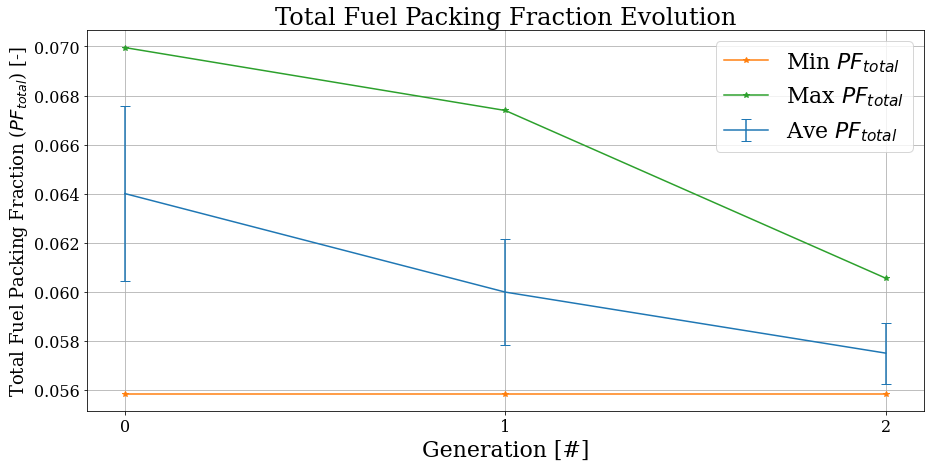
\includegraphics[width=\linewidth]{assem-obj-1-pf-evol.png}
        \caption{Minimum, average, and maximum $PF_{total}$ evolution.}
        \label{fig:assem-obj-1-pf-evol} 
    \end{subfigure}
    \begin{subfigure}{\textwidth}
        \centering
        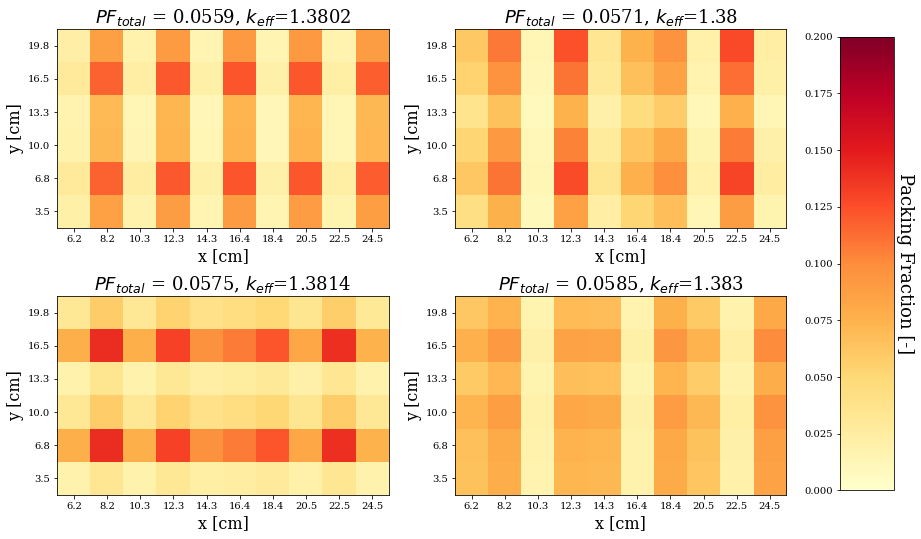
\includegraphics[width=\linewidth]{assem-obj-1-pf-final.png}
        \caption{TRISO packing fraction distribution for four unique reactor models with the 
        smallest $PF_{total}$ in the final generation.}
        \label{fig:assem-obj-1-pf-final} 
    \end{subfigure}
    \caption{Simulation a-1a -- ROLLO single-objective optimization to minimize total 
    fuel packing fraction ($PF_{total}$) in \gls{AHTR} one-third assembly. 
    Input parameters varied: $PF_{total}$, \gls{TRISO} packing fraction 
    distribution ($\rho_{TRISO}(\vec{r})$).}
    \label{fig:assem-obj-1-pf}
\end{figure}
\begin{figure}[htbp!]
    \ContinuedFloat
    \begin{subfigure}{\textwidth}
        \centering
        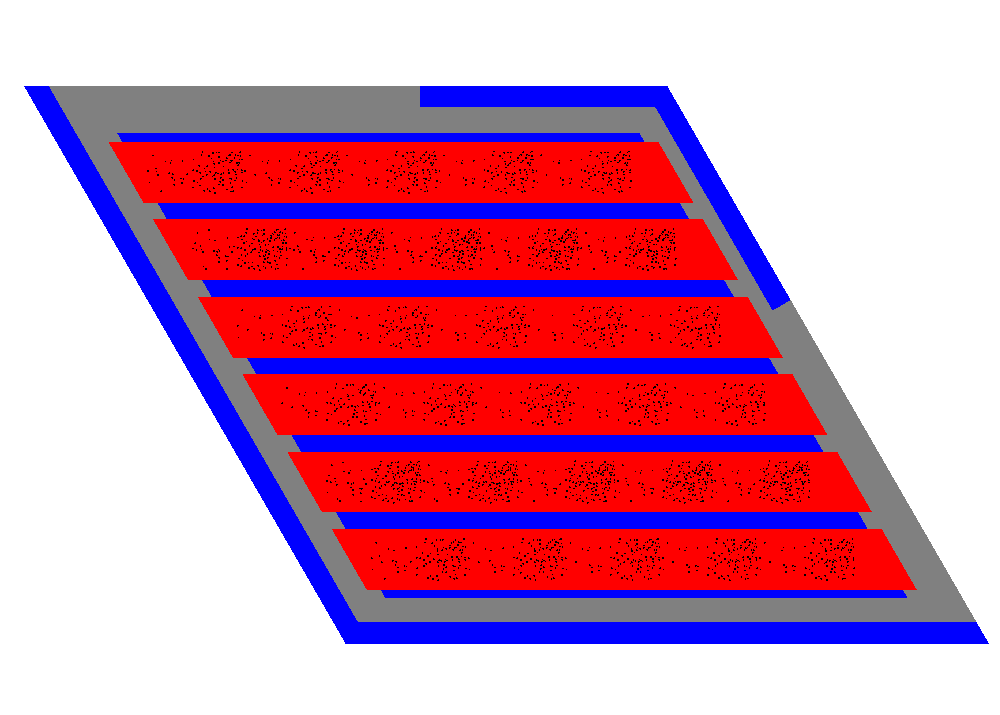
\includegraphics[width=0.7\linewidth]{assem-obj-1-pf-most-minimized.png}
        \caption{\gls{AHTR} one-third assembly model with the most-minimized 
        $PF_{total}$, corresponding to the top left TRISO distribution in Figure 
        \ref{fig:assem-obj-1-pf-final}. The reactor model has $PF_{total}=0.0559$
        and $k_{eff}=1.3802$.}
        \label{fig:assem-obj-1-pf-most-minimized} 
    \end{subfigure}
    \caption{(contd.) Simulation a-1a -- ROLLO single-objective optimization to minimize total 
    fuel packing fraction ($PF_{total}$) in \gls{AHTR} one-third assembly. 
    Input parameters varied: total fuel packing fraction 
    ($PF_{total}$), \gls{TRISO} packing fraction distribution ($\rho_{TRISO}(\vec{r})$).}
\end{figure}
Figure \ref{fig:assem-obj-1-pf-evol} shows that the minimum and average $PF_{total}$ 
converged to approximately 0.057 in the final generation. 
In Figure \ref{fig:assem-obj-1-pf-final}, the four unique TRISO packing fraction 
distributions in the final generation that most-minimized $PF_{total}$ have various 
oscillating TRISO distribution patterns. 

The one-third assembly model with the most-minimized $PF_{total}$ has a 
$PF_{total} =0.0559$, an oscillating TRISO distribution along the 
x-axis and y-axis, and a packing fraction standard deviation of $0.04$ across the 
one-third assembly. 
Along the x-axis, the distribution peaks on the even fuel cell columns (at 8.2cm, 12.3cm, 
16.4cm, 20.5cm, and 24.5cm). 
The even columns have the largest y-axis variation of ${\sim}0.05$ with peaks of
$PF\approx0.12$.
The odd columns have the smallest y-axis variation of ${\sim}0.01$ with minimums of 
$PF\approx0.01$.
Along the y-axis, the distribution peaks on the 2nd and 5th fuel cell rows (at 6.8cm and 
16.5cm).
The 2nd and 5th row have the largest x-axis variation of ${\sim}0.10$ with peaks of 
$PF\approx0.12$. 
The middle 3rd and 4th rows have the smallest x-axis variation of ${\sim}0.06$ with 
minimums of $PF\approx0.01$.
Because it is more productive to compare all of the single objective results to one 
another, Section \ref{sec:assem-discussion-single} discusses the driving factors for
the minimize $PF_{total}$ objective and explains simulation a-1a's most-minimized 
$PF_{total}$ oscillating TRISO distribution. 

\subsubsection{Simulation a-1d: Variation of $PF_{total}$ and Coolant channel shape}
Table \ref{tab:simulationa1d} summarizes simulation a-1d's optimization problem parameters. 
\begin{table}[htbp!]
    \centering
    \onehalfspacing
    \caption{Simulation a-1d Optimization Problem Parameters}
	\label{tab:simulationa1d}
    \footnotesize
    \begin{tabular}{l|p{6cm}}
    \hline 
    \multicolumn{2}{c}{\textbf{Single Objective: Simulation a-1d}} \\
    \hline 
    \textbf{Objectives} & Minimize $PF_{total}$ \\
    \hline 
    \textbf{Input Parameter variations} & $0.01<PF_{total}<0.04$ \\
    & coolant channel shape: $0.05<r_{1}<0.35$ \\
    & coolant channel shape: $0.05<r_{2}<0.35$ \\
    & coolant channel shape: $0.05<r_{3}<0.35$ \\
    & coolant channel shape: $0.05<r_{4}<0.35$ \\
    & coolant channel shape: $0.05<r_{5}<0.35$ \\
    \hline
    \textbf{Constraints} & $k_{eff} \geq 1.0$\\ 
    \hline 
    \textbf{Genetic Algorithm Parameters} & Population size: 64 \\
    & Generations: 2 \\
    \hline
    \end{tabular}
\end{table}
To remind readers each r value's orientation, Figure 
\ref{fig:coolant-channel-shape-assem-2} shows an annotated \gls{AHTR} one-third 
assembly's inter-plank coolant channel shapes for 
$r_1, r_2, r_3, r_4, r_5 = 0.3, 0.2, 0.1, 0.2, 0.3$.
\begin{figure}[htbp]
    \centering
    \begin{subfigure}{.8\textwidth}
    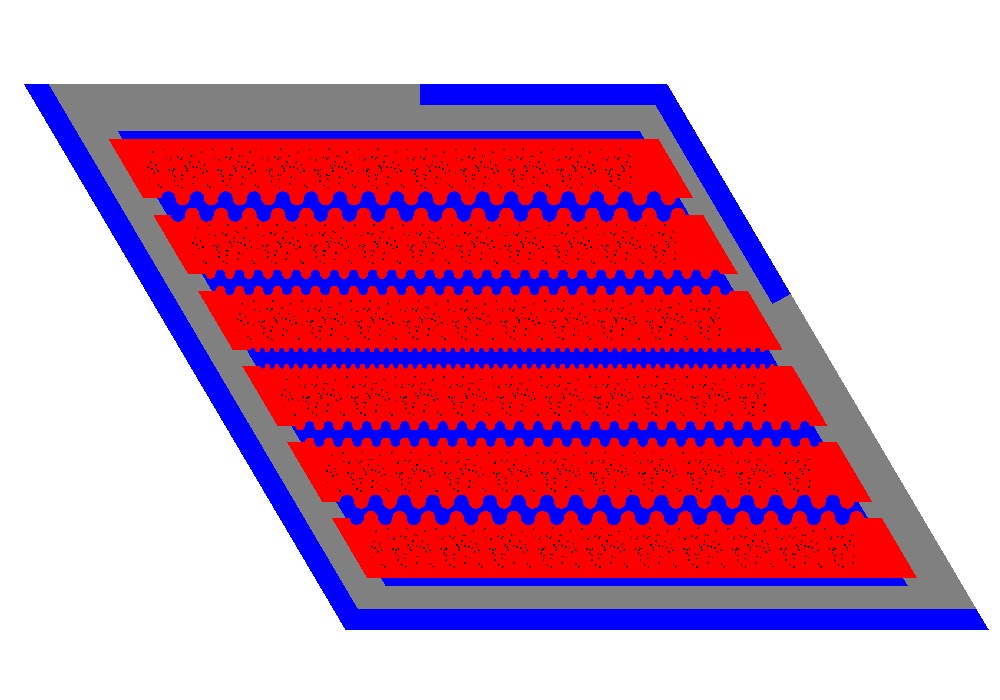
\includegraphics[width=\linewidth]{coolant-channel-shape-assem.png}
    \end{subfigure}%
    \begin{subfigure}{.2\textwidth}
        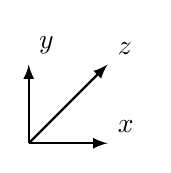
\begin{tikzpicture}
            \draw[ thick,-latex] (0,0) -- (1,0) node[anchor=south west] {$x$};
            \draw[ thick,-latex] (0,0) -- (0,1) node[anchor=south west] {$y$};
            \draw[ thick,-latex] (0,0) -- (1,1) node[anchor=south west] {$z$};
           \tkzText[above](-0.3,-0.7){}
        \end{tikzpicture} 
        \vspace{1cm}
        \resizebox{1.2\textwidth}{!}{
        \fbox{\begin{tabular}{ll}
            \textcolor{fhrblue}{$\blacksquare$} & \gls{FLiBe} \\
            \textcolor{fhrgrey}{$\blacksquare$} & Graphite (structure)\\
            \textcolor{fhrred}{$\blacksquare$} & Graphite (fuel plank) \\
            \textcolor{fhrblack}{$\blacksquare$} & TRISO particle 
            \end{tabular}}}
    \end{subfigure}
    \caption{\acrfull{AHTR} one-third assembly example with coolant channel shape 
    variation, $r_1, r_2, r_3, r_4, r_5 = 0.3cm, 0.2cm, 0.1cm, 0.2cm, 0.3cm$.}
    \label{fig:coolant-channel-shape-assem-2}
\end{figure}

Figure \ref{fig:a-1d} shows the plots of coolant channel shape's 
$r_1, r_2, r_3, r_4,$ and $r_5$ values against $PF_{total}$. 
\begin{figure}[htbp!]
    \centering
    \begin{subfigure}{0.49\textwidth}
        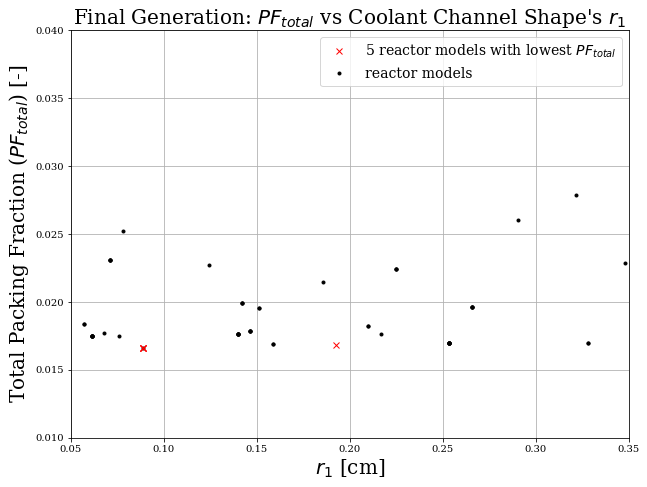
\includegraphics[width=\linewidth]{a-1d-r1.png}
        \caption{Plot of $PF_{total}$ against $r_1$.}
        \label{fig:a-1d-r1} 
    \end{subfigure}
    \begin{subfigure}{0.49\textwidth}
        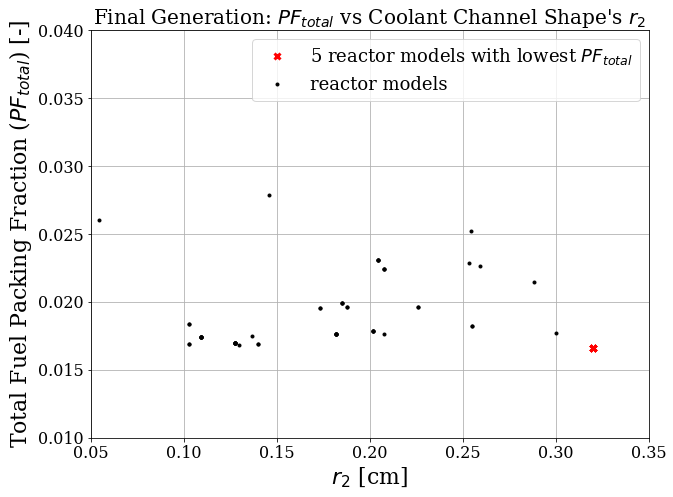
\includegraphics[width=\linewidth]{a-1d-r2.png}
        \caption{Plot of $PF_{total}$ against $r_2$.}
        \label{fig:a-1d-r2} 
    \end{subfigure}
    \begin{subfigure}{0.49\textwidth}
        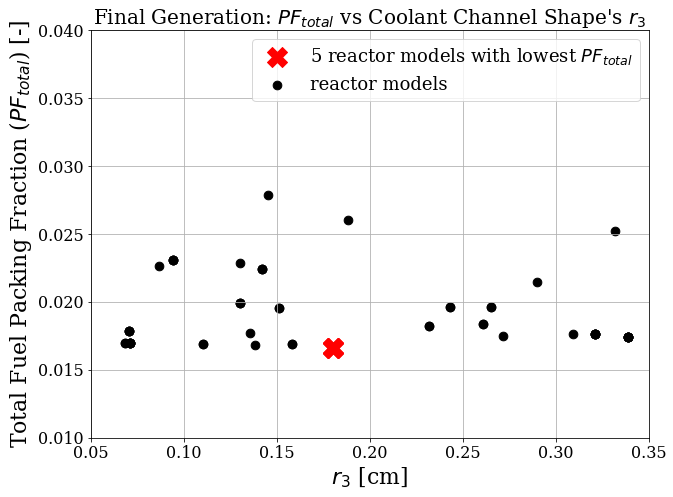
\includegraphics[width=\linewidth]{a-1d-r3.png}
        \caption{Plot of $PF_{total}$ against $r_3$.}
        \label{fig:a-1d-r3} 
    \end{subfigure}
    \begin{subfigure}{0.49\textwidth}
        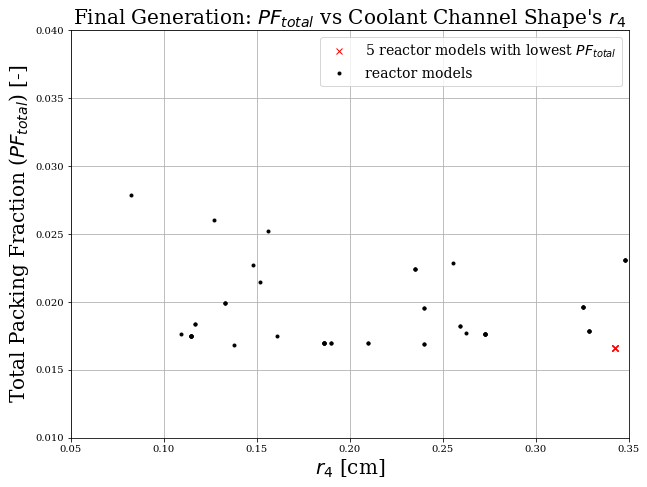
\includegraphics[width=\linewidth]{a-1d-r4.png}
        \caption{Plot of $PF_{total}$ against $r_4$.}
        \label{fig:a-1d-r4} 
    \end{subfigure}
    \begin{subfigure}{0.49\textwidth}
        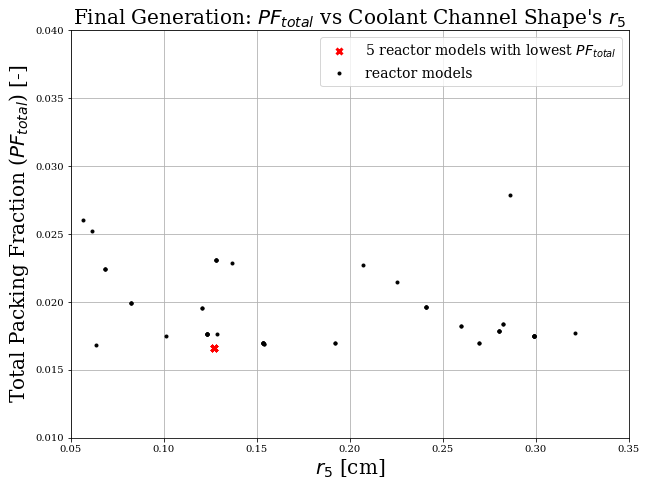
\includegraphics[width=\linewidth]{a-1d-r5.png}
        \caption{Plot of $PF_{total}$ against $r_5$.}
        \label{fig:a-1d-r5} 
    \end{subfigure}
    \caption{Simulation a-1d -- ROLLO single-objective optimization to minimize 
    total fuel packing fraction ($PF_{total}$). 
    Plots of simulation a-1d final generation's reactor models $PF_{total}$ against 
    coolant channel shape input parameters. 
    Red crosses indicate the five reactor models with the lowest $PF_{total}$.
    There is only red cross shown each plot because the five reactor models with the 
    lowest $PF_{total}$ are the same and overlap.
    Input parameters varied:
    $PF_{total}$ and coolant channel shape ($r_1, r_2, r_3, r_4, r_5$).}
    \label{fig:a-1d}
\end{figure}
The random scattering of reactor model points in Figure \ref{fig:a-1d}
demonstrates that there is no correlation between $PF_{total}$ 
and coolant channel shape's $r_1, r_2, r_3, r_4,$ and $r_5$. 

\subsection{Objective: Minimize Maximum Temperature ($T_{max}$)}
\label{sec:assem-1-obj-temp}
This section reports results from the minimize maximum one-third assembly temperature 
($T_{max}$) single-objective optimization simulations: a-1b and a-1e. 
Simulation a-1b varies \gls{TRISO} packing fraction distribution 
($\rho_{TRISO}(\vec{r})$), and simulation a-1e varies the coolant channel shape
($r_1, r_2, r_3, r_4,$ and $r_5$). 

\subsubsection{Simulation a-1b: Variation of $\rho_{TRISO}(\vec{r})$}
Table \ref{tab:simulationa1b} summarizes simulation a-1b's optimization problem parameters. 
\begin{table}[htbp!]
    \centering
    \onehalfspacing
    \caption{Simulation a-1b Optimization Problem Parameters}
	\label{tab:simulationa1b}
    \footnotesize
    \begin{tabular}{l|p{5.3cm}}
    \hline 
    \multicolumn{2}{c}{\textbf{Single Objective: Simulation a-1b}} \\
    \hline 
    \textbf{Objectives} & Minimize $T_{max}$ \\
    \hline 
    \textbf{Input Parameter variations} 
    & $\rho_{TRISO}(\vec{r})$: $0 \leq a \leq 2$, $0 \leq d \leq 2$\\
    & $\rho_{TRISO}(\vec{r})$: $0 \leq b \leq \frac{\pi}{2}$, $0 \leq e \leq \frac{\pi}{2}$\\
    & $\rho_{TRISO}(\vec{r})$: $0 \leq c \leq 2\pi$, $0 \leq f \leq 2\pi$\\
    \hline
    \textbf{Constraints} & $k_{eff} \geq 1.38$\\ 
    & $PF_{total} = 0.06 $\\ 
    \hline 
    \textbf{Genetic Algorithm Parameters} & Population size: 128 \\
    & Generations: 3 \\
    \hline
    \end{tabular}
\end{table}
Figure \ref{fig:assem-obj-1-temp-evol} shows the one-third assembly's $T_{max}$ 
evolution. 
Figure \ref{fig:assem-obj-1-temp-final} shows four unique TRISO packing fraction 
distributions in the final generation with the most minimized $T_{max}$. 
Figure \ref{fig:assem-obj-1-temp-most-minimized} illustrates the \gls{AHTR} one-third 
assembly model with the most-minimized $T_{max}$. 
\begin{figure}[htbp!]
    \begin{subfigure}{\textwidth}
        \centering
        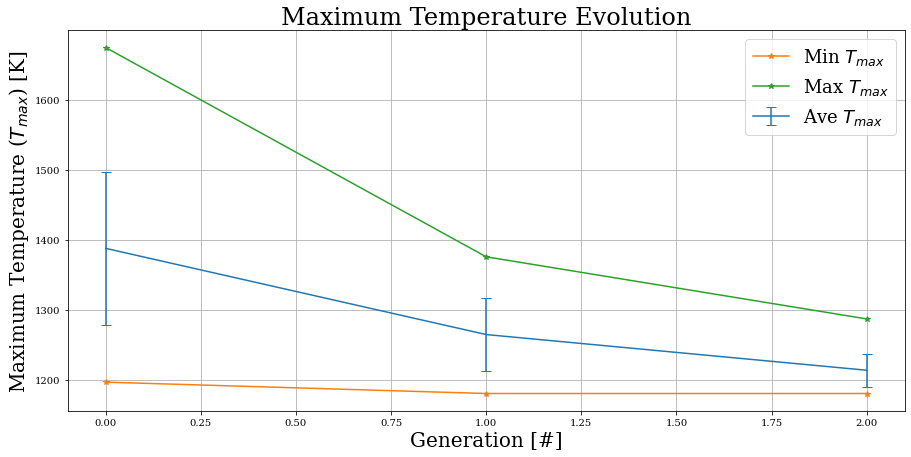
\includegraphics[width=\linewidth]{assem-obj-1-temp-evol.png}
        \caption{Minimum, average, and maximum $T_{max}$ evolution.}
        \label{fig:assem-obj-1-temp-evol} 
    \end{subfigure}
    \begin{subfigure}{\textwidth}
        \centering
        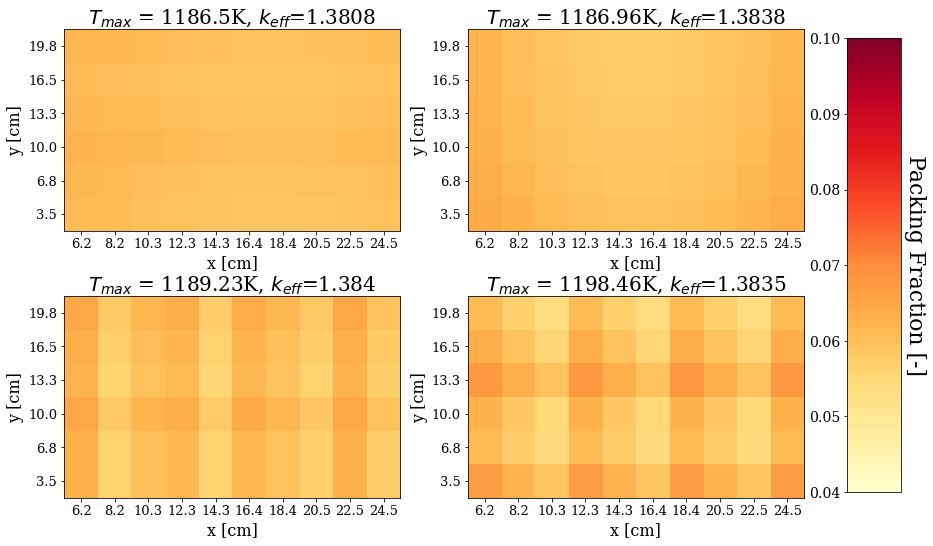
\includegraphics[width=\linewidth]{assem-obj-1-temp-final.png}
        \caption{TRISO packing fraction distribution for four unique reactor models with the 
        smallest $T_{max}$ in the final generation.}
        \label{fig:assem-obj-1-temp-final} 
    \end{subfigure}
    \caption{Simulation a-1b -- ROLLO single-objective optimization to minimize maximum 
    temperature ($T_{max}$) in the \gls{AHTR} one-third assembly. 
    Input parameters varied: \gls{TRISO} packing fraction distribution 
    ($\rho_{TRISO}(\vec{r})$).}
    \label{fig:assem-obj-1-temp}
\end{figure}
\begin{figure}[htbp!]
    \ContinuedFloat
    \begin{subfigure}{\textwidth}
        \centering
        \begin{subfigure}{0.7\textwidth}
            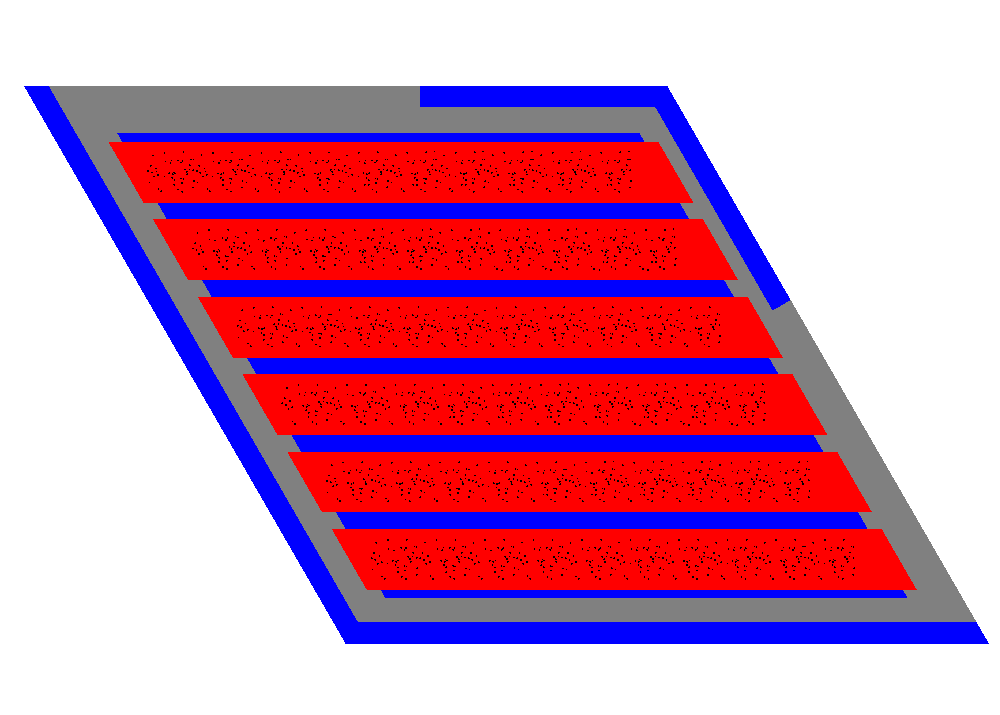
\includegraphics[width=\linewidth]{assem-obj-1-temp-most-minimized.png}
            \end{subfigure}%
            \begin{subfigure}[t]{.3\textwidth}
                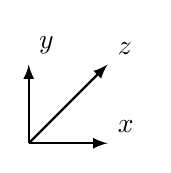
\begin{tikzpicture}
                    \draw[ thick,-latex] (0,0) -- (1,0) node[anchor=south west] {$x$};
                    \draw[ thick,-latex] (0,0) -- (0,1) node[anchor=south west] {$y$};
                    \draw[ thick,-latex] (0,0) -- (1,1) node[anchor=south west] {$z$};
                   \tkzText[above](-0.3,-0.7){}
                \end{tikzpicture} 
            \end{subfigure}
        \caption{\gls{AHTR} one-third assembly model with the most-minimized 
        $T_{max}$, corresponding to the top left TRISO distribution in Figure 
        \ref{fig:assem-obj-1-temp-final}. The reactor model has $T_{max}=1180.29$K
        and $k_{eff}=1.3046$.}
        \label{fig:assem-obj-1-temp-most-minimized} 
    \end{subfigure}
    \caption{Simulation a-1b -- ROLLO single-objective optimization to minimize maximum 
    temperature ($T_{max}$) in \gls{AHTR} one-third assembly. 
    Input parameters varied: \gls{TRISO} packing fraction distribution 
    ($\rho_{TRISO}(\vec{r})$).}
\end{figure}

Some key features that can be observed in Figure \ref{fig:assem-obj-1-temp-evol} are 
that the minimum and average one-third assembly's $T_{max}$ converged to approximately 
1200 K.
In Figure \ref{fig:assem-obj-1-temp-final}, the one-third assembly model with the 
most-minimized $T_{max}$ has a $T_{max}=1186.5$K and an almost constant TRISO packing 
fraction distribution with packing fraction standard deviation of $0.0009$ across the 
one-third assembly. 
Because it is more productive to compare all of the single objective results to one 
another, Section \ref{sec:plank-discussion-single} discusses and explains simulation 
p-1b's most-minimized $T_{max}$ almost constant TRISO distribution. 

\subsubsection{Simulation a-1e: Variation of Coolant channel shape}
Table \ref{tab:simulationa1e} summarizes simulation a-1e's optimization problem parameters. 
\begin{table}[htbp!]
    \centering
    \onehalfspacing
    \caption{Simulation a-1e Optimization Problem Parameters}
	\label{tab:simulationa1e}
    \footnotesize
    \begin{tabular}{l|p{6cm}}
    \hline 
    \multicolumn{2}{c}{\textbf{Single Objective: Simulation a-1e}} \\
    \hline 
    \textbf{Objectives} & Minimize $T_{max}$ \\
    \hline 
    \textbf{Input Parameter variations} 
    & coolant channel shape: $0.05<r_{1}<0.35$ \\
    & coolant channel shape: $0.05<r_{2}<0.35$ \\
    & coolant channel shape: $0.05<r_{3}<0.35$ \\
    & coolant channel shape: $0.05<r_{4}<0.35$ \\
    & coolant channel shape: $0.05<r_{5}<0.35$ \\
    \hline
    \textbf{Constraints} & $k_{eff} \geq 1.38$\\ 
    & $PF_{total} = 0.06 $\\ 
    \hline 
    \textbf{Genetic Algorithm Parameters} & Population size: 128 \\
    & Generations: 2 \\
    \hline
    \end{tabular}
\end{table}
To remind readers each r value's orientation, Figure 
\ref{fig:coolant-channel-shape-assem-2} shows an annotated \gls{AHTR} one-third 
assembly's inter-plank coolant channel shapes for 
$r_1, r_2, r_3, r_4, r_5 = 0.3, 0.2, 0.1, 0.2, 0.3$.

Figure \ref{fig:a-1e-evol} shows the one-third assembly's $T_{max}$ evolution.
Figure \ref{fig:assem-obj-1-temp-most-minimized-coolant} illustrates the \gls{AHTR} 
one-third assembly model with the most-minimized $T_{max}$. 
Figures \ref{fig:a-1e-r1}, \ref{fig:a-1e-r2}, \ref{fig:a-1e-r3}, \ref{fig:a-1e-r4}, 
and \ref{fig:a-1e-r5} show the plots of coolant channel shape's 
$r_1, r_2, r_3, r_4,$ and $r_5$ values against $T_{max}$. 
\begin{figure}[htbp!]
    \begin{subfigure}{\textwidth}
        \centering
        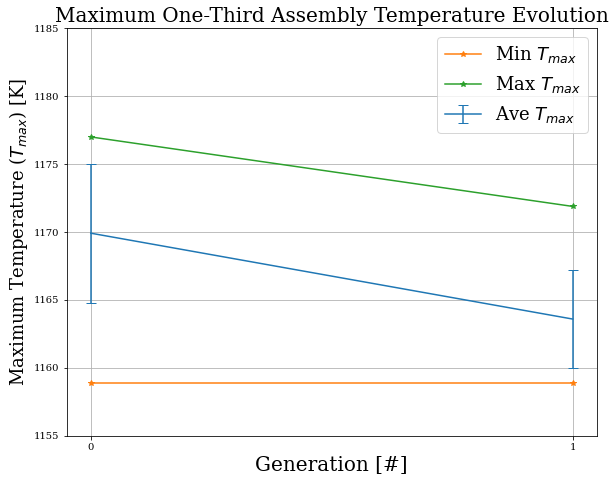
\includegraphics[width=\linewidth]{a-1e-evol.png}
        \caption{Minimum, average, and maximum evolution of AHTR one-third assembly's 
        $T_{max}$.}
        \label{fig:a-1e-evol} 
    \end{subfigure}
    \begin{subfigure}{\textwidth}
        \centering
        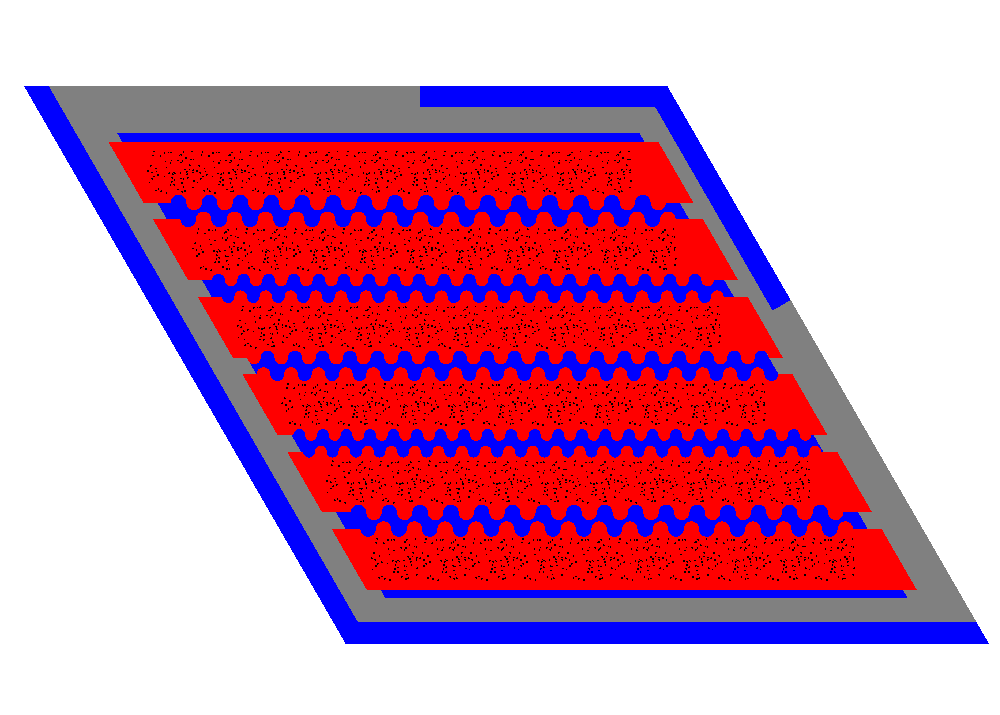
\includegraphics[width=0.8\linewidth]{assem-obj-1-temp-most-minimized-coolant.png}
        \caption{\gls{AHTR} one-third assembly model with the most-minimized $T_{max}$. 
        The reactor model has $T_{max} = 1161.28K$, $r_1 = 0.32cm$, $r_{2} = 0.26cm$,
        $r_3 = 0.28cm$, $r_{4} = 0.24cm$, and $r_{5} = 0.32cm$.}
        \label{fig:assem-obj-1-temp-most-minimized-coolant} 
    \end{subfigure}
    \caption{Simulation a-1e -- ROLLO single-objective optimization to minimize 
    maximum one-third assembly temperature ($T_{max}$). 
    Plots of final generation's reactor models $T_{max}$ against 
    coolant channel shape input parameters. 
    Red crosses indicate the five reactor models with the lowest $T_{max}$.
    Input parameters varied: coolant channel shape ($r_1, r_2, r_3, r_4, r_5$).}
    \label{fig:a-1e}
\end{figure}
\begin{figure}[htbp!]
    \ContinuedFloat
    \centering
    \begin{subfigure}{0.49\textwidth}
        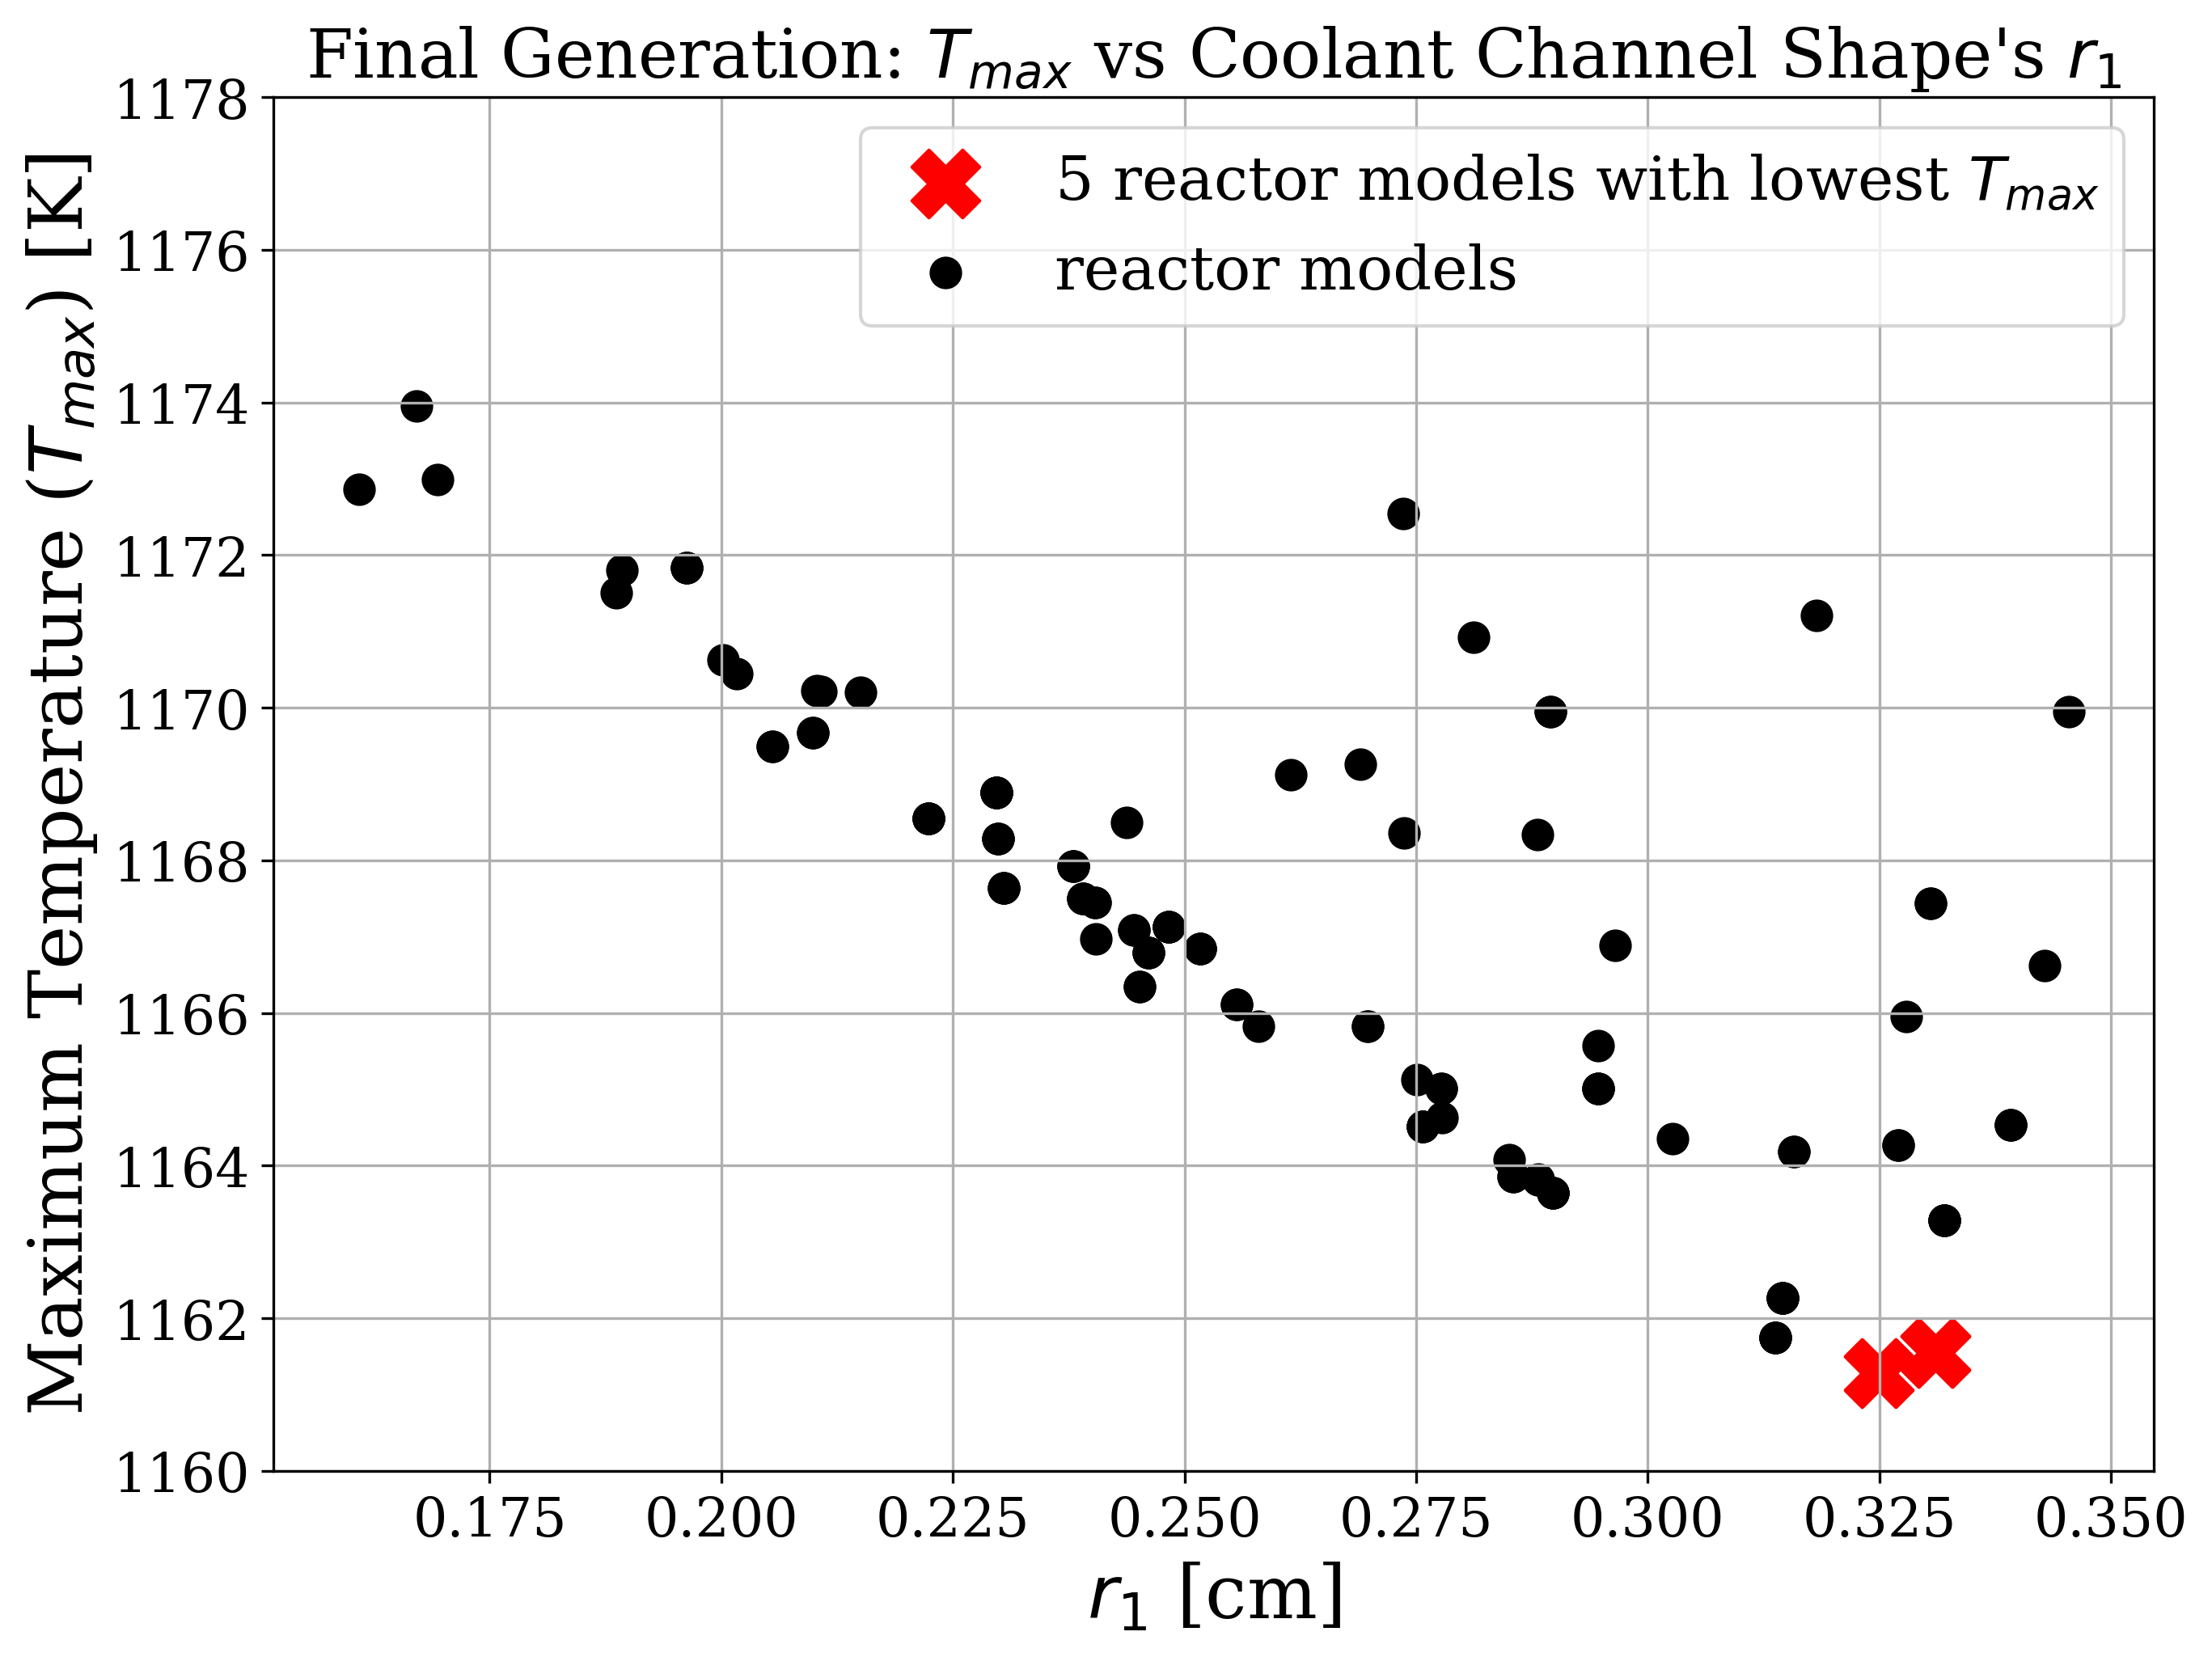
\includegraphics[width=\linewidth]{a-1e-r1.png}
        \caption{Plot of $PF_{total}$ against $r_1$.}
        \label{fig:a-1e-r1} 
    \end{subfigure}
    \begin{subfigure}{0.49\textwidth}
        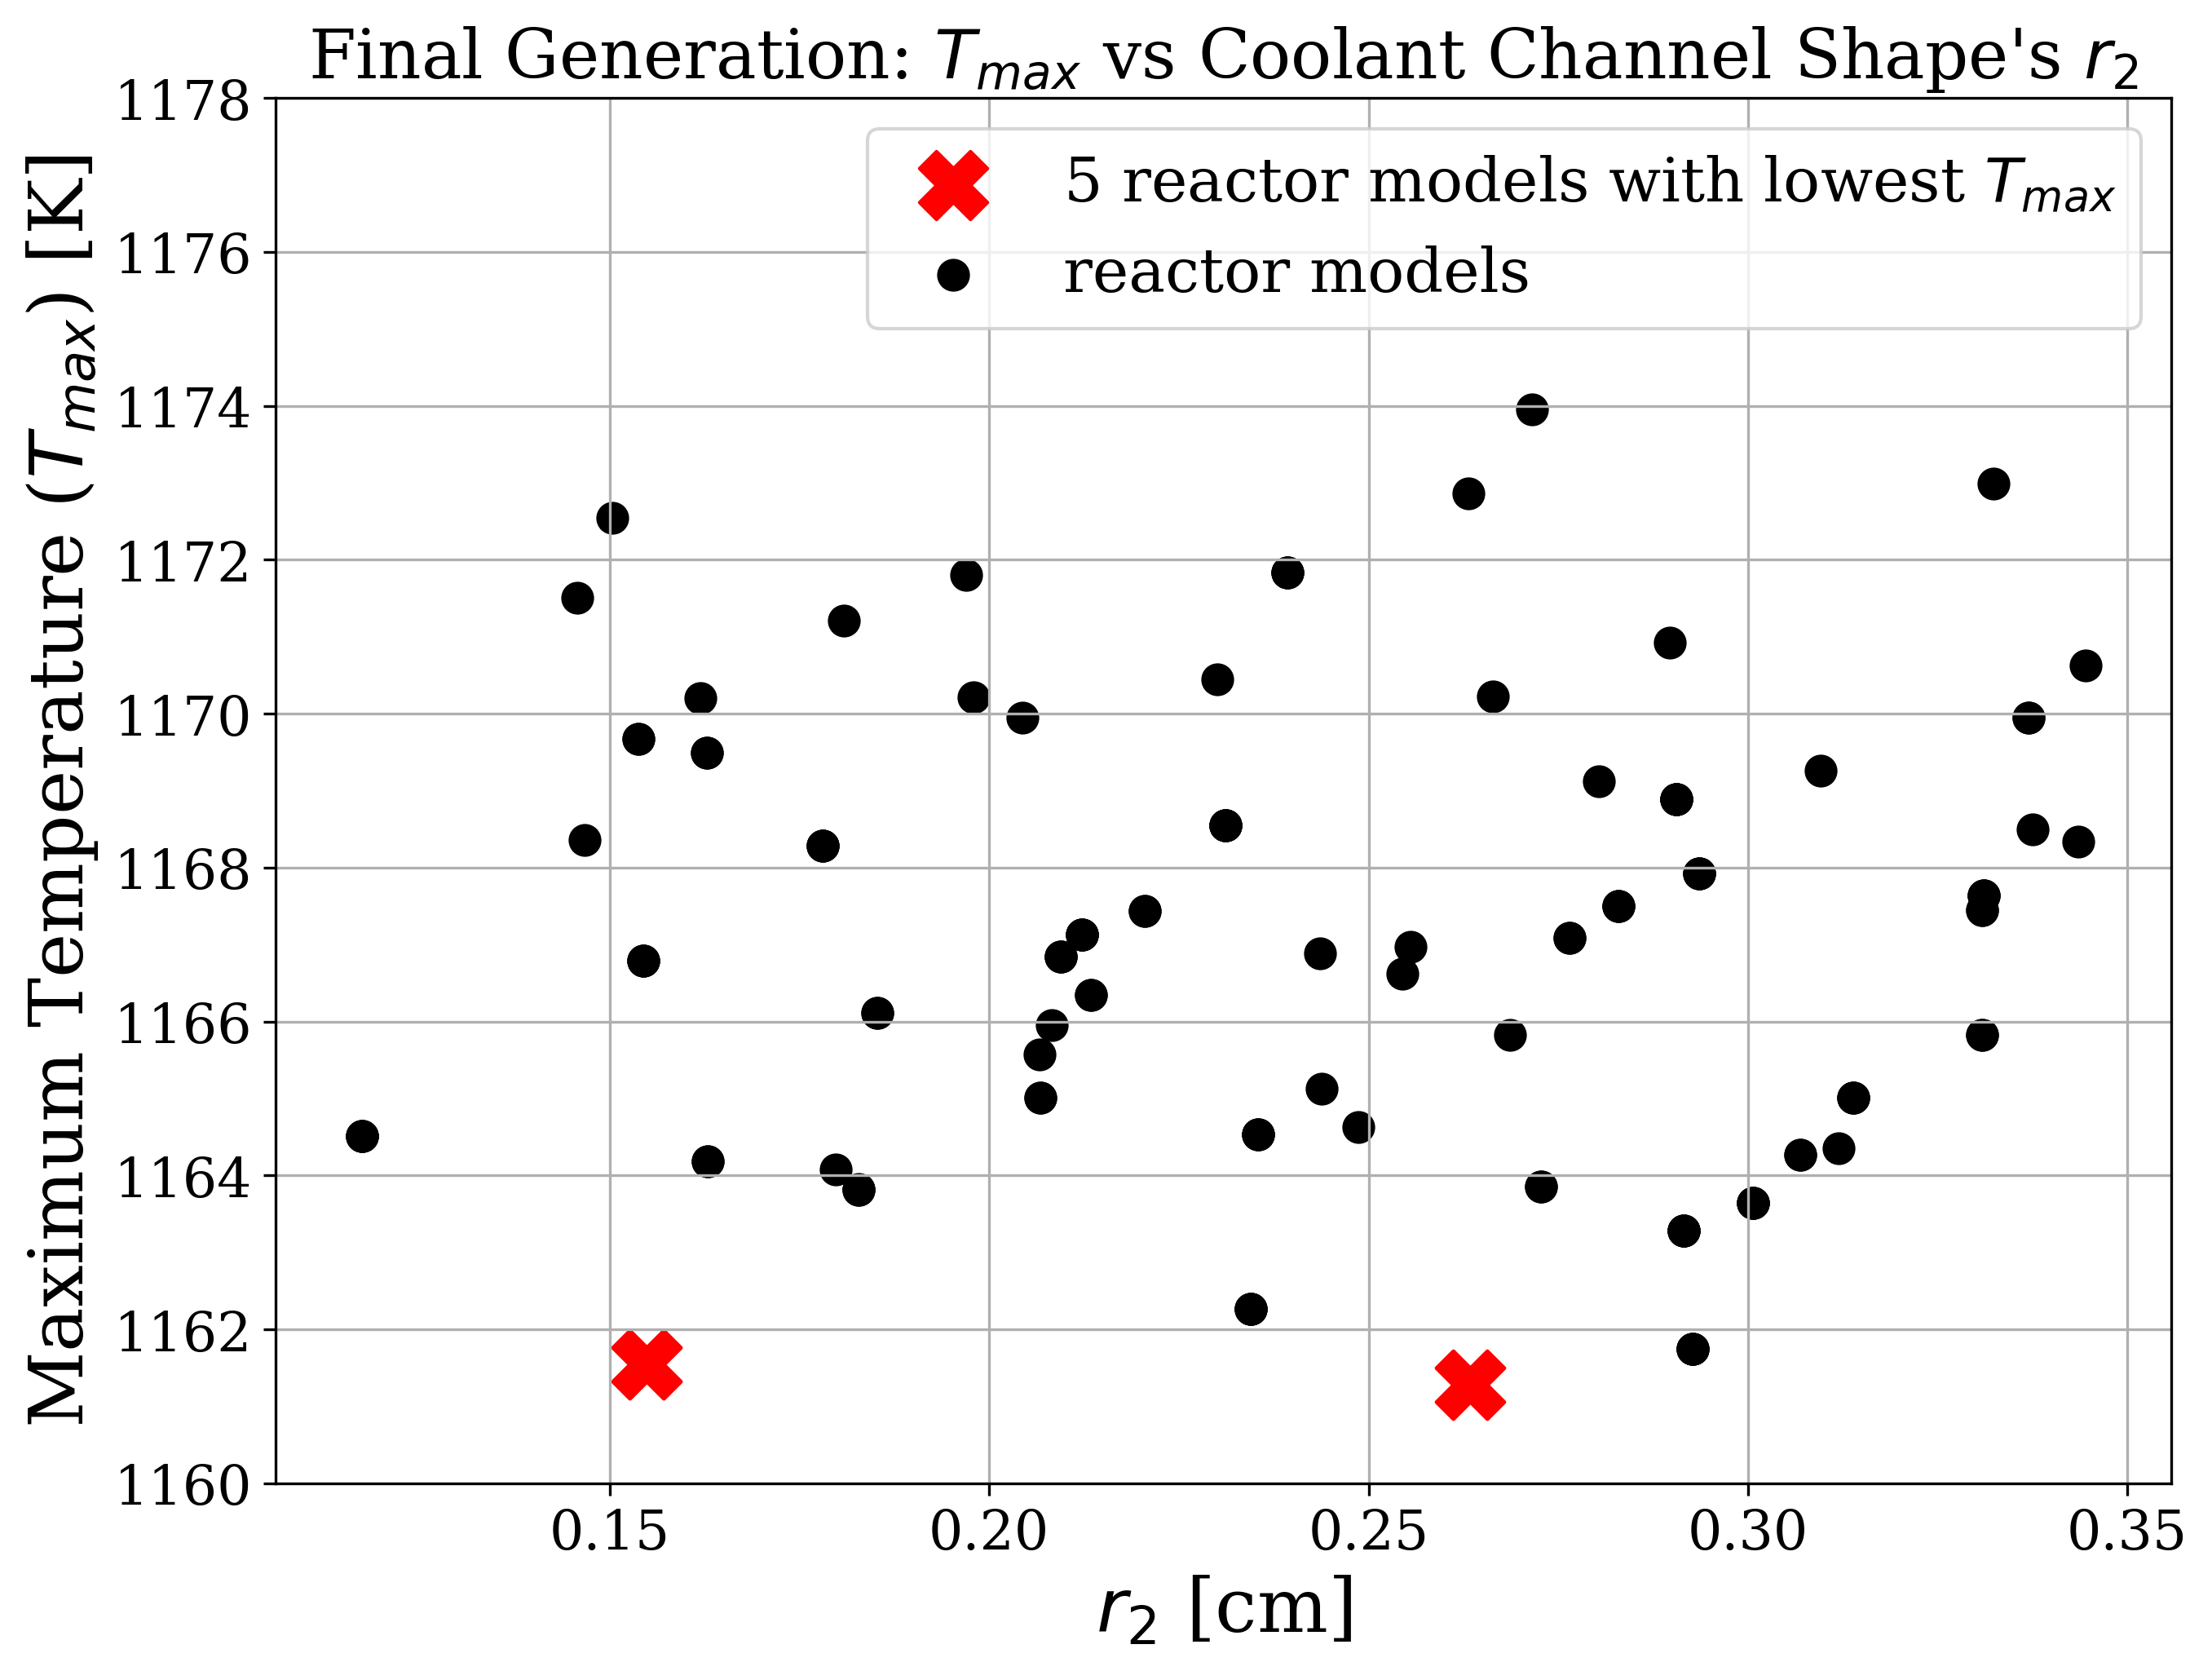
\includegraphics[width=\linewidth]{a-1e-r2.png}
        \caption{Plot of $PF_{total}$ against $r_2$.}
        \label{fig:a-1e-r2} 
    \end{subfigure}
    \begin{subfigure}{0.49\textwidth}
        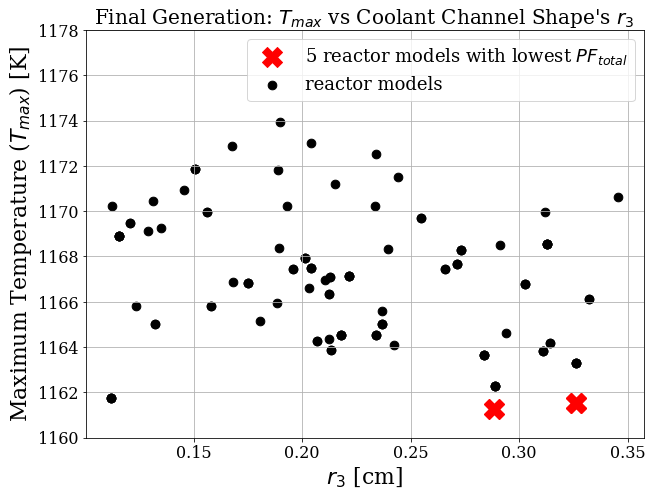
\includegraphics[width=\linewidth]{a-1e-r3.png}
        \caption{Plot of $PF_{total}$ against $r_3$.}
        \label{fig:a-1e-r3} 
    \end{subfigure}
    \begin{subfigure}{0.49\textwidth}
        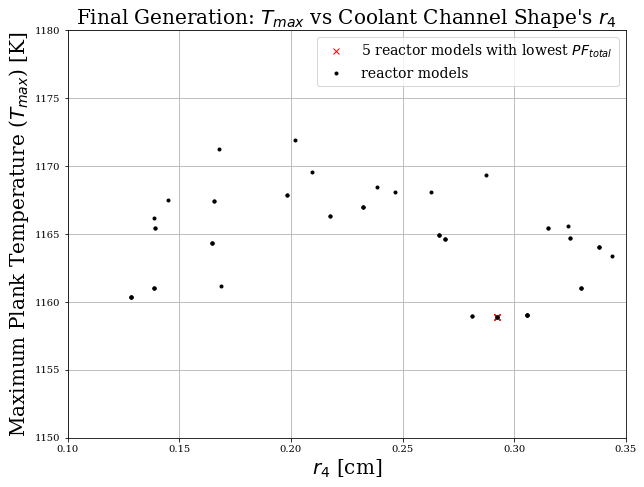
\includegraphics[width=\linewidth]{a-1e-r4.png}
        \caption{Plot of $PF_{total}$ against $r_4$.}
        \label{fig:a-1e-r4} 
    \end{subfigure}
    \begin{subfigure}{0.49\textwidth}
        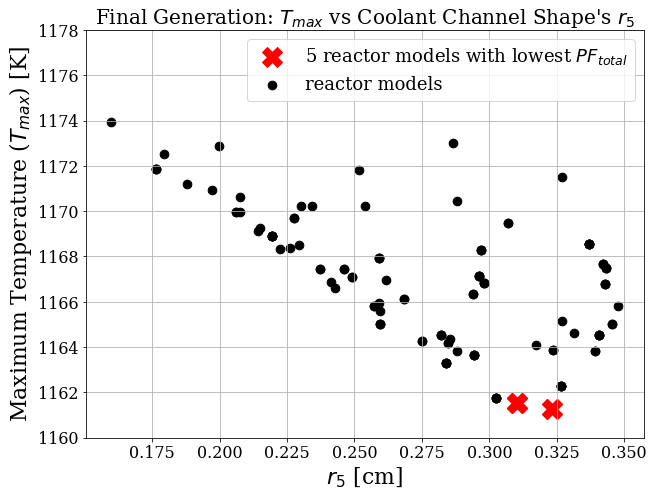
\includegraphics[width=\linewidth]{a-1e-r5.png}
        \caption{Plot of $PF_{total}$ against $r_5$.}
        \label{fig:a-1e-r5} 
    \end{subfigure}
    \caption{Simulation a-1e -- ROLLO single-objective optimization to minimize 
    maximum one-third assembly temperature ($T_{max}$). 
    Plots of final generation's reactor models $T_{max}$ against 
    coolant channel shape input parameters. 
    Red crosses indicate the five reactor models with the lowest $T_{max}$.
    Some of the five reactor models with the lowest $T_{max}$ are the same, thus 
    their crosses overlap.
    Input parameters varied: coolant channel shape ($r_1, r_2, r_3, r_4, r_5$).}
\end{figure}

Figures \ref{fig:a-1e-r1} and \ref{fig:a-1e-r5} demonstrate negative linear 
correlations between the one-third assembly's $T_{max}$ with $r_1$ and $r_5$. 
The random scattering of reactor model points in Figures \ref{fig:a-1e-r2}, 
\ref{fig:a-1e-r3} and \ref{fig:a-1e-r4} demonstrate that 
there is no correlation between $T_{max}$ with $r_2$, $r_3$, and $r_4$. 
Section \ref{sec:assen-discussion-single} discusses and explains the relationship 
between $T_{max}$ and coolant channel shape. 

\subsection{Objective: Minimize Fuel-Normalized Power Peaking Factor ($PPF_{fuel}$)}
\label{sec:assem-1-obj-ppf}
This section reports the minimize fuel-normalized power peaking factor 
($PPF_{fuel}$) single-objective optimization simulation results: a-1c and a-1f. 
Simulation a-1c varies \gls{TRISO} packing fraction distribution 
($\rho_{TRISO}(\vec{r})$), and simulation a-1f varies the coolant channel shape 
($r_1, r_2, r_3, r_4,$ and $r_5$).

\subsubsection{Simulation a-1c: Variation of $\rho_{TRISO}(\vec{r})$}
Table \ref{tab:simulationa1c} summarizes simulation a-1c's optimization problem parameters. 
\begin{table}[htbp!]
    \centering
    \onehalfspacing
    \caption{Simulation a-1c Optimization Problem Parameters}
	\label{tab:simulationa1c}
    \footnotesize
    \begin{tabular}{l|p{5.3cm}}
    \hline 
    \multicolumn{2}{c}{\textbf{Single Objective: Simulation a-1c}} \\
    \hline 
    \textbf{Objectives} & Minimize $PPF_{fuel}$ \\
    \hline 
    \textbf{Input Parameter variations}
    & $\rho_{TRISO}(\vec{r})$: $0 \leq a \leq 2$, $0 \leq d \leq 2$\\
    & $\rho_{TRISO}(\vec{r})$: $0 \leq b \leq \frac{\pi}{2}$, $0 \leq e \leq \frac{\pi}{2}$\\
    & $\rho_{TRISO}(\vec{r})$: $0 \leq c \leq 2\pi$, $0 \leq f \leq 2\pi$\\
    \hline
    \textbf{Constraints} & $k_{eff} \geq 1.38$\\ 
    & $PF_{total}$ = 0.06 \\
    \hline 
    \textbf{Genetic Algorithm Parameters} & Population size: 128 \\
    & Generations: 2 \\
    \hline
    \end{tabular}
\end{table}
Figure \ref{fig:assem-obj-1-ppf-evol} shows the one-third assembly's $PPF_{fuel}$ 
evolution. 
Figure \ref{fig:assem-obj-1-ppf-final} shows the four unique TRISO packing fraction 
distributions in the final generation with the most minimized $PPF_{fuel}$. 
Figure \ref{fig:assem-obj-1-ppf-most-minimized} illustrates the \gls{AHTR} one-third 
assembly model with the most-minimized $PPF_{fuel}$. 
\begin{figure}[htbp!]
    \begin{subfigure}{\textwidth}
        \centering
        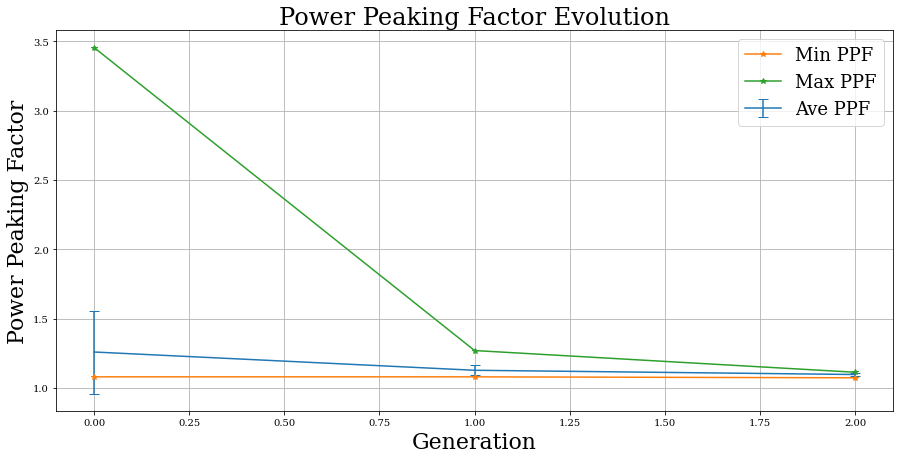
\includegraphics[width=\linewidth]{assem-obj-1-ppf-evol.png}
        \caption{Minimum, average, and maximum evolution of $PPF_{fuel}$ in the 
        AHTR one-third assembly.}
        \label{fig:assem-obj-1-ppf-evol} 
    \end{subfigure}
    \begin{subfigure}{\textwidth}
        \centering
        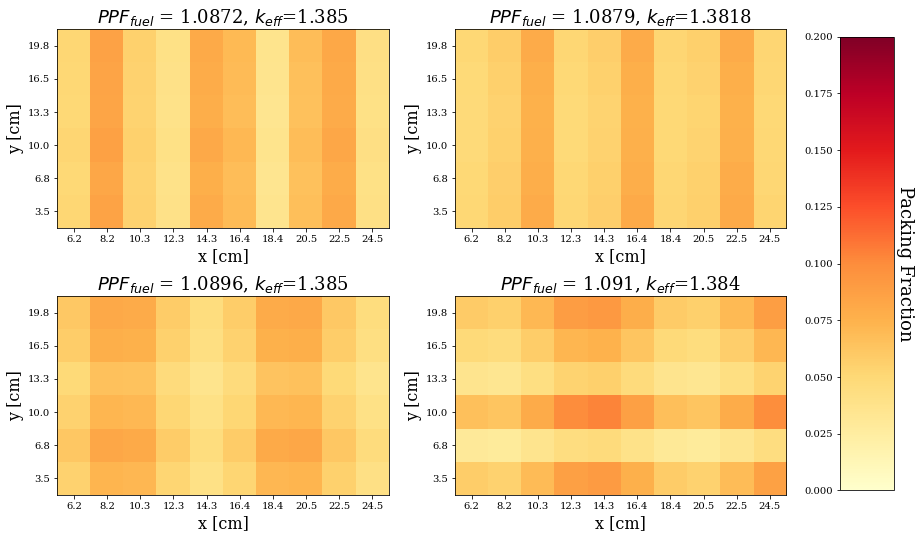
\includegraphics[width=\linewidth]{assem-obj-1-ppf-final.png}
        \caption{TRISO distribution for the four unique reactor models with the 
        lowest $PPF_{fuel}$ in the AHTR one-third assembly at the final generation.}
        \label{fig:assem-obj-1-ppf-final} 
    \end{subfigure}
    \caption{Simulation a-1c -- ROLLO single-objective optimization to minimize 
    AHTR one-third assembly's fuel-normalized power peaking factor ($PPF_{fuel}$). 
    Input parameters varied: TRISO distribution ($\rho_{TRISO}(\vec{r})$).
    $PF_{total}$ = 0.06.}
    \label{fig:assem-obj-1-ppf}
\end{figure}
\begin{figure}[htbp!]
    \ContinuedFloat
    \begin{subfigure}{\textwidth}
        \centering
        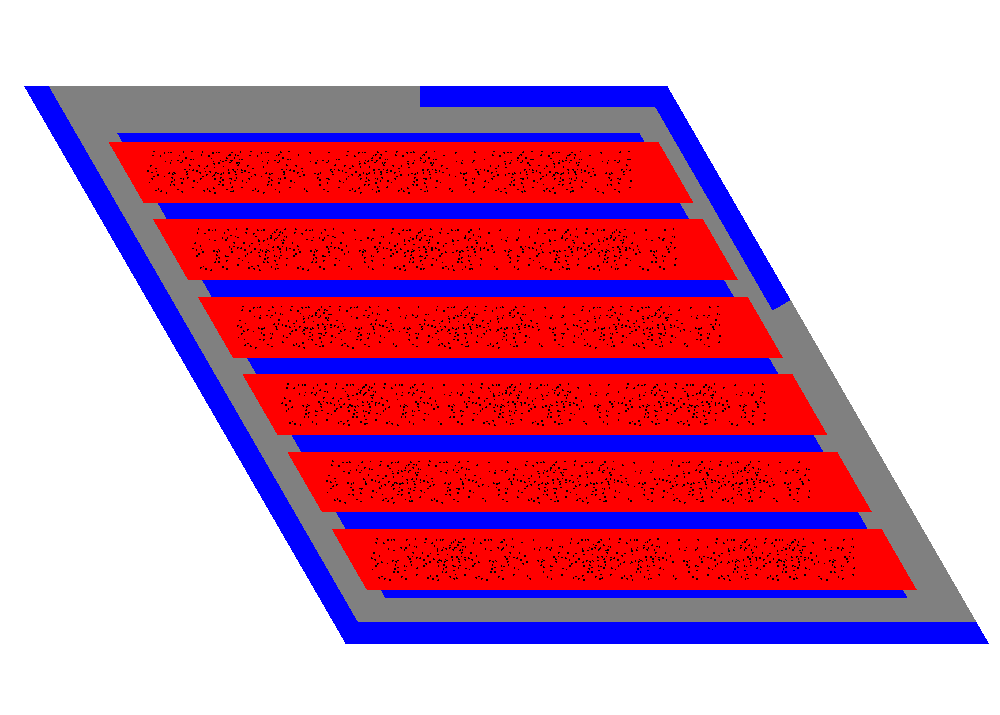
\includegraphics[width=0.7\linewidth]{assem-obj-1-ppf-most-minimized.png}
        \caption{\gls{AHTR} one-third assembly model with the most-minimized 
        $PPF_{fuel}$, corresponding to the top left TRISO distribution in Figure 
        \ref{fig:assem-obj-1-ppf-final}. The reactor model has $PPF_{fuel}=1.0872$
        and $k_{eff}=1.385$.}
        \label{fig:assem-obj-1-ppf-most-minimized} 
    \end{subfigure}
    \caption{Simulation a-1c -- ROLLO single-objective optimization to minimize 
    AHTR one-third assembly's fuel-normalized power peaking factor ($PPF_{fuel}$). 
    Input parameters varied: TRISO distribution ($\rho_{TRISO}(\vec{r})$).
    $PF_{total}$ = 0.06.}
\end{figure}

Features of note in Figure \ref{fig:assem-obj-1-ppf-evol} are that the minimum and 
average one-third assembly's $PPF_{fuel}$ converged to approximately 1.1.
In Figure \ref{fig:assem-obj-1-ppf-final}, the most-minimized TRISO distribution has 
a $PPF_{fuel} = 1.0872$ and an oscillating TRISO distribution along the x-axis and a 
packing fraction standard deviation of $0.017$ across the one-third assembly. 
Along the x-axis, the distribution peaks at the 2nd, 5th, and 9th fuel 
cell columns (at 8.2cm, 14.3cm, and 22.5cm) with $PF\approx0.08$ and has minimum points
at the 4th and 7th fuel cell columns (at 12.3cm and 18.4cm) with $PF\approx0.035$. 
Section \ref{sec:assen-discussion-single} discusses the driving factors for the minimize 
$PPF_{fuel}$ objective and explains simulation a-1c's most-minimized $PPF_{fuel}$ 
TRISO distribution. 

\subsubsection{Simulation a-1f: Variation of Coolant channel shape}
Table \ref{tab:simulationa1f} summarizes simulation a-1f's optimization problem parameters. 
\begin{table}[htbp!]
    \centering
    \onehalfspacing
    \caption{Simulation a-1f Optimization Problem Parameters}
	\label{tab:simulationa1f}
    \footnotesize
    \begin{tabular}{l|p{6cm}}
    \hline 
    \multicolumn{2}{c}{\textbf{Single Objective: Simulation a-1f}} \\
    \hline 
    \textbf{Objectives} & Minimize $PPF_{fuel}$ \\
    \hline 
    \textbf{Input Parameter variations} 
    & coolant channel shape: $0.05<r_{1}<0.35$ \\
    & coolant channel shape: $0.05<r_{2}<0.35$ \\
    & coolant channel shape: $0.05<r_{3}<0.35$ \\
    & coolant channel shape: $0.05<r_{4}<0.35$ \\
    & coolant channel shape: $0.05<r_{5}<0.35$ \\
    \hline
    \textbf{Constraints} & $k_{eff} \geq 1.0$\\ 
    & $PF_{total}$ = 0.04 \\
    \hline 
    \textbf{Genetic Algorithm Parameters} & Population size: 64 \\
    & Generations: 2 \\
    \hline
    \end{tabular}
\end{table}
To remind readers each r value's orientation, Figure 
\ref{fig:coolant-channel-shape-assem-2} shows an annotated \gls{AHTR} one-third 
assembly's inter-plank coolant channel shapes for 
$r_1, r_2, r_3, r_4, r_5 = 0.3, 0.2, 0.1, 0.2, 0.3$.

Figure \ref{fig:a-1f} shows the plots of coolant channel shape's 
$r_1, r_2, r_3, r_4,$ and $r_5$ values against $PPF_{fuel}$. 
\begin{figure}[htbp!]
    \centering
    \begin{subfigure}{0.49\textwidth}
        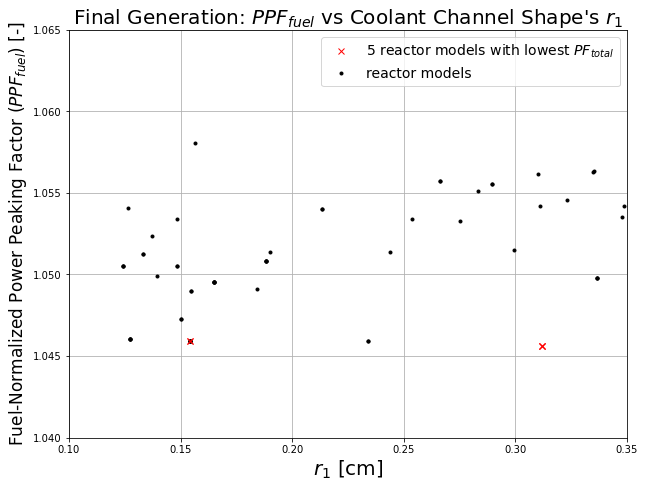
\includegraphics[width=\linewidth]{a-1f-r1.png}
        \caption{Plot of $PF_{total}$ against $r_1$.}
        \label{fig:a-1f-r1} 
    \end{subfigure}
    \begin{subfigure}{0.49\textwidth}
        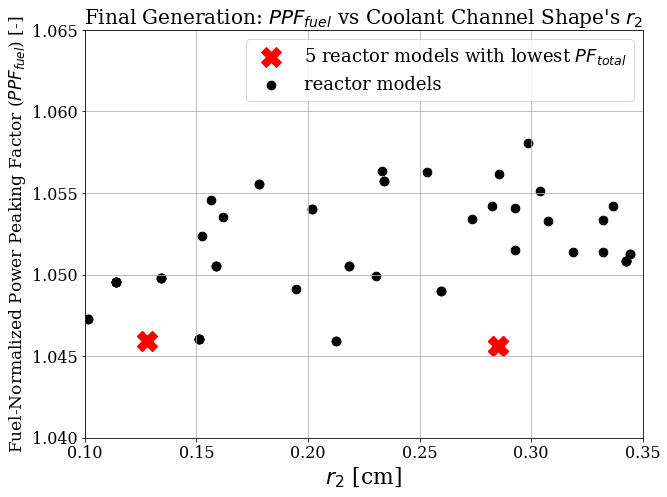
\includegraphics[width=\linewidth]{a-1f-r2.png}
        \caption{Plot of $PF_{total}$ against $r_2$.}
        \label{fig:a-1f-r2} 
    \end{subfigure}
    \begin{subfigure}{0.49\textwidth}
        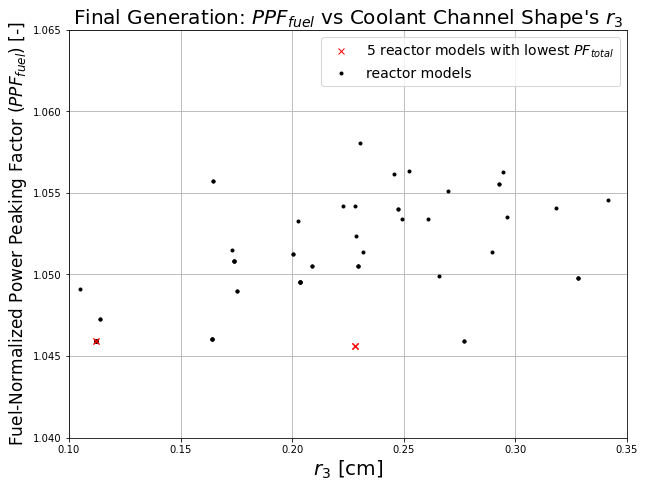
\includegraphics[width=\linewidth]{a-1f-r3.png}
        \caption{Plot of $PF_{total}$ against $r_3$.}
        \label{fig:a-1f-r3} 
    \end{subfigure}
    \begin{subfigure}{0.49\textwidth}
        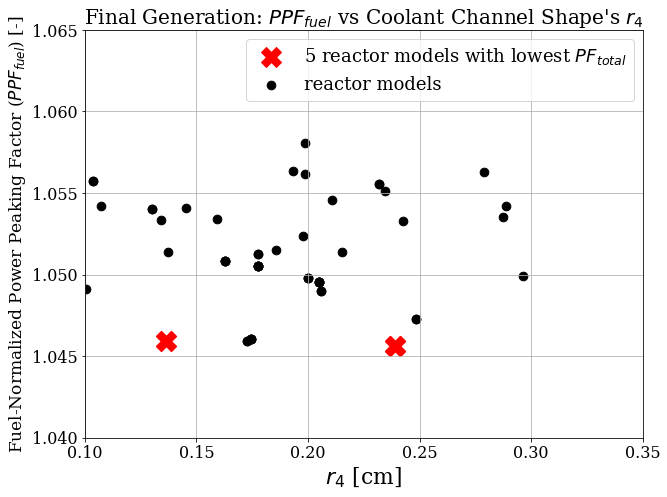
\includegraphics[width=\linewidth]{a-1f-r4.png}
        \caption{Plot of $PF_{total}$ against $r_4$.}
        \label{fig:a-1f-r4} 
    \end{subfigure}
    \begin{subfigure}{0.49\textwidth}
        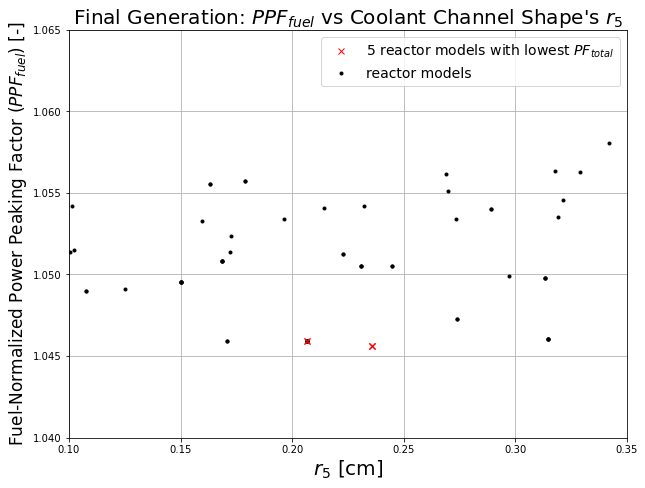
\includegraphics[width=\linewidth]{a-1f-r5.png}
        \caption{Plot of $PF_{total}$ against $r_5$.}
        \label{fig:a-1f-r5} 
    \end{subfigure}
    \caption{Simulation a-1f -- ROLLO single-objective optimization to minimize 
    AHTR one-third assembly's fuel-normalized power peaking factor ($PPF_{fuel}$). 
    Plots of simulation a-1f final generation's reactor models $PPF_{fuel}$ against 
    coolant channel shape input parameters. 
    Red crosses indicate the five reactor models with the lowest $PPF_{fuel}$.
    Some of the five reactor models with the lowest $PPF_{fuel}$ are the same, thus 
    their crosses overlap.
    Input parameters varied: total fuel packing fraction 
    ($PPF_{fuel}$), and coolant channel shape ($r_1, r_2, r_3, r_4, r_5$).}
    \label{fig:a-1f}
\end{figure}
The random scattering of reactor model points in Figure \ref{fig:a-1f} demonstrates 
that there is no correlation between $PPF_{fuel}$ and coolant channel shape's 
$r_1, r_2, r_3, r_4,$ and $r_5$. 

\subsection{Single-Objective Optimization Discussion}
\label{sec:assem-discussion-single}
Chapter \ref{chap:ahtr-plank-opt-results} characterized the \gls{AHTR} plank model's 
reactor optimization objectives' driving factors and their relationship with 
one another. 
This section utilizes the previous \gls{AHTR} plank characterizations and conducts 
a comparative analysis to verify if the same driving factors apply to the 
\gls{AHTR} one-third assembly model's optimization objectives. 

\subsubsection{Discussion: Minimize $PF_{total}$ Objective}
\paragraph{Simulation a-1a}
In Section \ref{sec:assem-1-obj-pf}'s simulation a-1a, I conducted a single-objective 
optimization simulation to minimize the one-third assembly's total fuel packing fraction 
($PF_{total}$) by varying $PF_{total}$ and TRISO distribution. 
\gls{ROLLO} found that an \gls{AHTR} one-third assembly model with 
the most-minimized $PF_{total}$ has a $PF_{total}= 0.0559$ and an oscillating TRISO 
distribution along the x-axis and y-axis, and a packing fraction standard 
deviation of $0.04$ across the one-third assembly (Figure \ref{fig:assem-obj-1-pf-final}).

Section \ref{sec:plank-discussion-pf} concluded that for the \gls{AHTR} plank model, 
the minimize $PF_{total}$ objective is driven by maximizing the total fission reaction 
rates. 
I ran a simulation for constant $PF_{total} = 0.0559$ TRISO distribution and compared its 
fission reaction rate with simulation a-1a's oscillating TRISO distribution that 
most-minimized $PF_{total}$. 
Figure \ref{fig:assem-0.0559-comparison} shows the TRISO distributions for the two 
compared reactor models: Figure \ref{fig:assem-obj-1-pf-final}'s most-minimized 
$PF_{total}$ and the constant $PF_{total} = 0.0559$. 
\begin{figure}[htbp!]
    \centering
    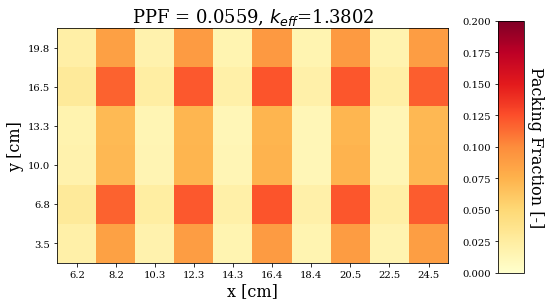
\includegraphics[width=0.49\linewidth]{assem-0.0559-most-minimized.png} 
    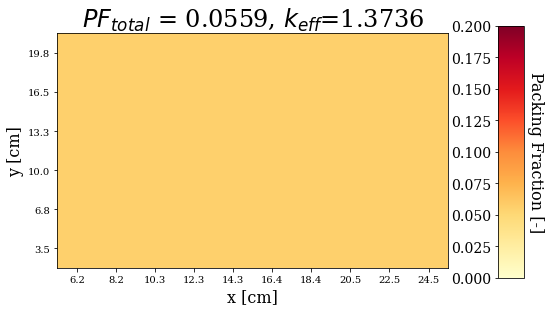
\includegraphics[width=0.49\linewidth]{assem-0.0559-flat.png} 
    \caption{Simulation a-1a's most-minimized $PF_{total}$ TRISO distribution 
    (oscillating TRISO distribution) from Figure \ref{fig:assem-obj-1-pf} (left) and the 
    constant $PF_{total} = 0.0559$ TRISO distribution (right).}
    \label{fig:assem-0.0559-comparison}
\end{figure}
The reactor model with the most-minimized $PF_{total}$ has $k_{eff}=1.3802$, and 
the reactor model with constant TRISO distribution has $k_{eff}=1.3736$.

Table \ref{tab:a-1a-fission-comparison} compares the total fission reaction rate 
(OpenMC's \texttt{fission} tally) between the most-minimized $PF_{total}$ TRISO 
distribution and a constant $PF_{total} = 0.0559$ TRISO distribution (both shown in 
Figure \ref{fig:assem-0.0559-comparison}).
\begin{table}[htbp!]
    \centering
    \onehalfspacing
    \caption{Total fission reaction rate comparison between simulation a-1a's 
    most-minimized $PF_{total}$ TRISO distribution and a constant $PF_{total} = 0.0559$ 
    TRISO distribution. Both distributions shown in Figure 
    \ref{fig:assem-0.0559-comparison}.}
	\label{tab:a-1a-fission-comparison}
    \footnotesize
    \begin{tabular}{p{1.5cm}lp{3.7cm}p{4cm}p{2.5cm}}
    \hline
    \textbf{Energy Group} & 
    \textbf{$\%$ of Total} &
    \textbf{Most-minimized $PF_{total}$ Fission \newline [reactions/src]} & 
    \textbf{Flat $PF_{total}$ Fission [reactions/src]} & 
    \textbf{$\%$ Fission \newline Difference}\\
    \hline 
    1 & 00.28 & 0.00165 & 0.00162 & \Plus2.01 \\
    2 & 01.56 & 0.00886 & 0.00884 & \Plus0.21 \\
    3 & 01.51 & 0.00854 & 0.00852 & \Plus0.23 \\
    4 & 96.63 & 0.54813 & 0.54465 & \Plus0.63 \\
    Total & - & 0.52998 & 0.52656 & \Plus0.65 \\
    \hline
    \end{tabular}
\end{table}
The most-minimized $PF_{total}$ TRISO distribution has $0.65\%$ higher  
total fission reaction rate than the constant $PF_{total} = 0.0559$ TRISO distribution. 
For the same $PF_{total}$, the oscillating TRISO distribution enabled
660pcm higher $k_{eff}$ than the constant TRISO distribution. 
The minimize $PF_{total}$ objective is driven by maximizing the total fission 
reaction rates to find a reactor model with lower $PF_{total}$ that meets $k_{eff}$ 
constraints. 

\paragraph{Simulation a-1d}
In Section \ref{sec:assem-1-obj-pf}'s simulation a-1d, I conducted a single-objective 
optimization simulation to minimize total fuel packing fraction ($PF_{total}$) by 
varying $PF_{total}$ and coolant channel shape. 
In simulation a-1d, \gls{ROLLO} found no correlation 
between $PF_{total}$ and coolant channel shape (demonstrated in Figure 
\ref{fig:a-1d}). 

\paragraph{Summary}
I confirmed that the minimize $PF_{total}$ objective for the \gls{AHTR} one-third 
assembly model is also driven by maximizing the total fission reaction rates. 
The minimize $PF_{total}$ objective influences oscillations in the TRISO distribution.
The objective does not correlate with the coolant channel shape.

\subsubsection{Discussion: Minimize $T_{max}$ Objective}
\paragraph{Simulation a-1b}
In Section \ref{sec:assem-1-obj-temp}'s simulation a-1b, I conducted a single-objective 
optimization simulation to minimize the one-third assembly's maximum temperature 
($T_{max}$) by varying TRISO distribution. 
In simulation a-1b, \gls{ROLLO} found that for $PF_{total}$ = 0.06, the reactor model 
with the most-minimized $T_{max}$ has a $T_{max} = 1161.28K$ with an almost constant 
TRISO distribution (Figure \ref{fig:assem-obj-1-temp-final}). 

\paragraph{Simulation a-1e}
In Section \ref{sec:assem-1-obj-temp}'s simulation a-1e, I conducted a single-objective 
optimization simulation to minimize the one-third assembly's maximum temperature 
($T_{max}$) by varying coolant channel shape. 
In simulation a-1e, \gls{ROLLO} found a negative linear correlation 
between the one-third assembly's $T_{max}$ and $r_1$ and $r_5$, but no correlation with 
$r_2$, $r_3$, and $r_4$, shown in Figure \ref{fig:a-1e}. 

Figures \ref{fig:a-1e-temp-distribution-2d} and \ref{fig:a-1e-temp-distribution-centerline}
show the 2D temperature distribution and centerline temperature for simulation a-1e's 
one-third assembly model with the most-minimized $T_{max}$ (Figure 
\ref{fig:assem-obj-1-temp-most-minimized-coolant}). 
% todo: fix plot no overlap. 
\begin{figure}[htbp!]
    \begin{subfigure}{\textwidth}
        \centering
        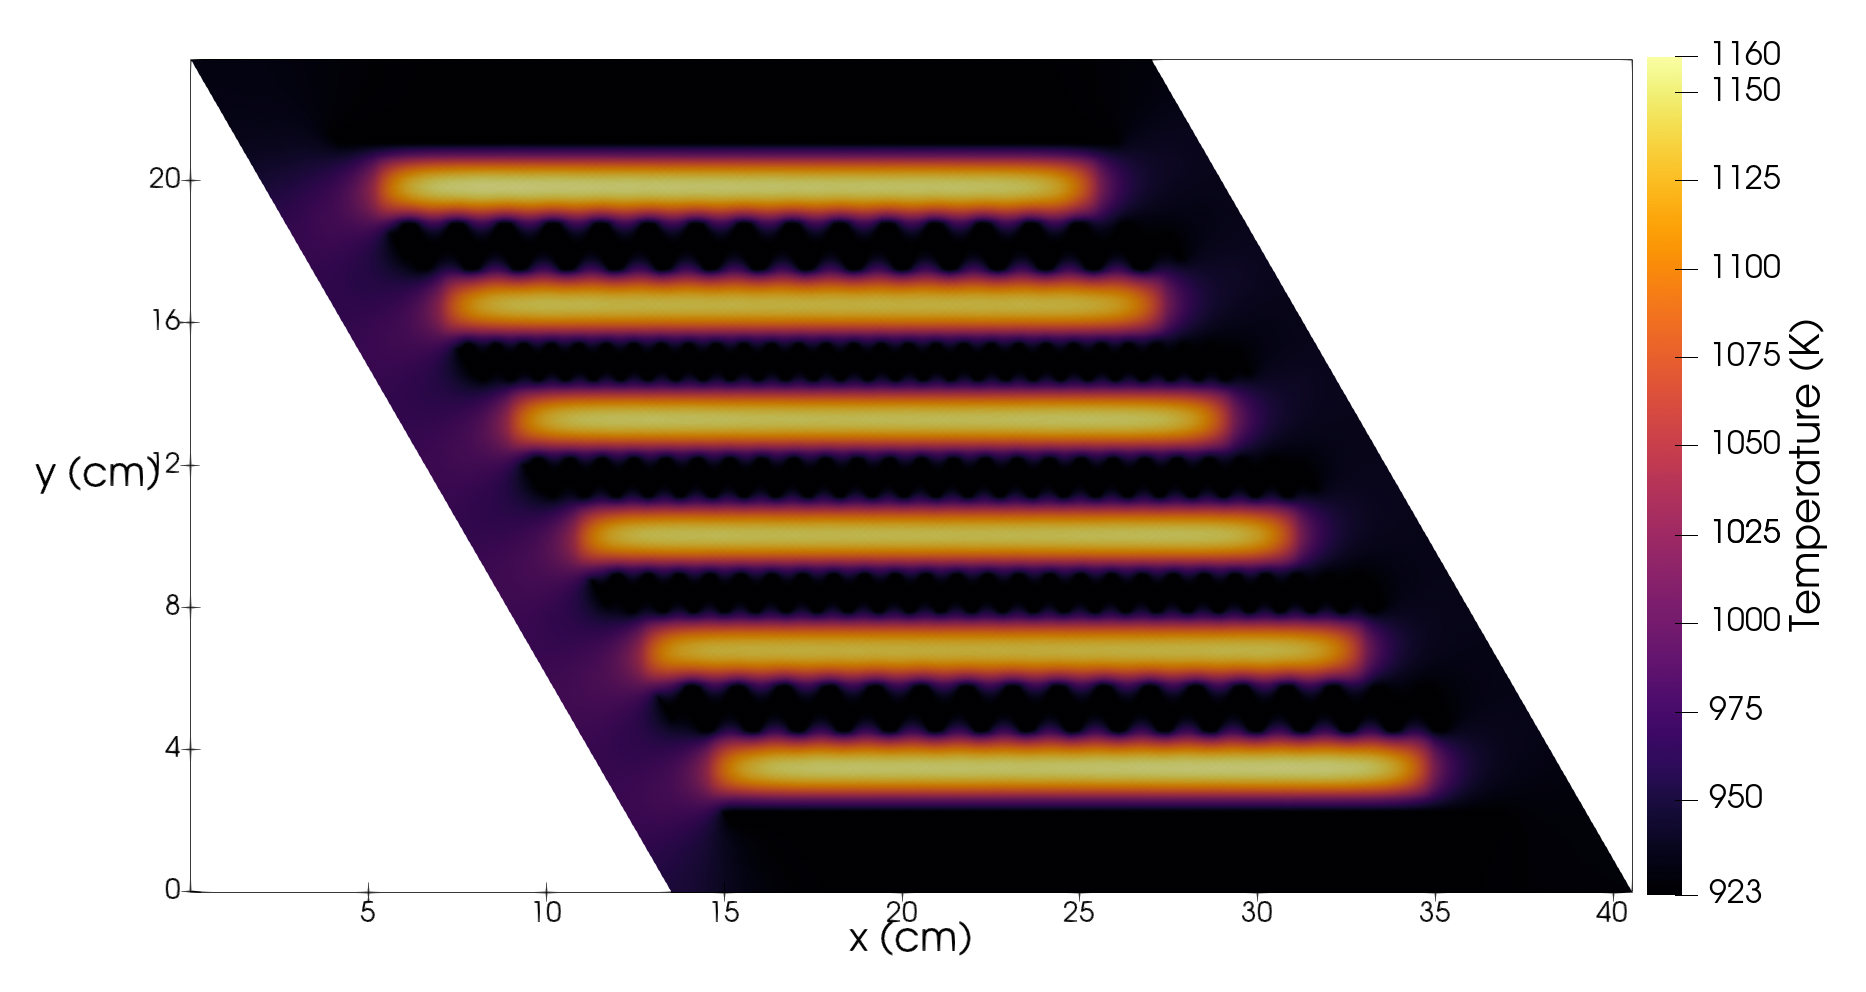
\includegraphics[width=\linewidth]{a-1e-temp-distribution-2d.png}
        \caption{2D temperature distribution.}
        \label{fig:a-1e-temp-distribution-2d} 
    \end{subfigure}
    \begin{subfigure}{\textwidth}
        \centering
        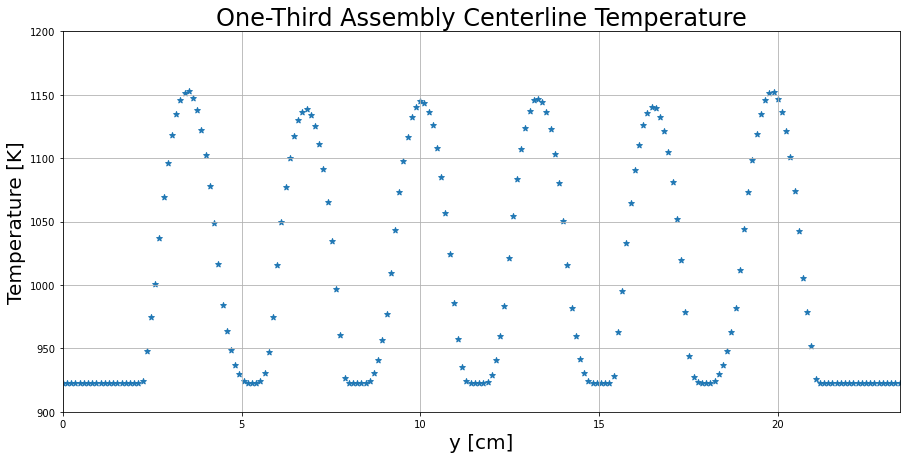
\includegraphics[width=\linewidth]{a-1e-temp-distribution-centerline.png}
        \caption{Centerline temperature. AHTR assembly's centerline is the white line 
        in Figure \ref{fig:ahtr-assem-verification}.}
        \label{fig:a-1e-temp-distribution-centerline} 
    \end{subfigure}
    \caption{Simulation a-1e's most-minimized $T_{max}$ one-third assembly reactor 
    model's temperature distribution.}
    \label{fig:a-1e-temp-distribution}
\end{figure}
Figure \ref{fig:a-1e-temp-distribution} demonstrates that for simulation a-1e's 
most-minimized $T_{max}$ reactor model, the temperature peaks in the top and bottom 
graphite planks. 
$r_1$ and $r_5$ control the coolant channel shape of the \gls{FLiBe} channels closest 
to the top and bottom graphite planks. 
This explains why \gls{ROLLO} found a negative linear correlation 
between the one-third assembly's $T_{max}$ and $r_1$ and $r_5$. 
To minimize the maximum one-third assembly temperature, \gls{ROLLO} maximized
$r_1$ and $r_5$ to enable enhanced cooling in the top and bottom graphite planks. 
Thus, depending on the temperature distribution in a one-third assembly, the \gls{FLiBe} 
channels (corresponding to $r_1, r_2, r_3, r_4, r_5$) closest to the temperature peaks 
will be most important to minimizing $T_{max}$. 

\paragraph{Summary}
I verified that, similar to the \gls{AHTR} plank model, a flatter TRISO distribution 
minimizes the one-third assembly's $T_{max}$. 
For the one-third assembly, the FLiBe channels (corresponding to $r_1, r_2, r_3, r_4, 
r_5$) closest to the temperature peaks will be most important to minimizing maximum
one-third assembly temperature and thus, will show a negative correlation with 
$T_{max}$. 
Simulation a-1b and a-1e suggest that TRISO distribution influences the minimize 
$T_{max}$ objective more than the coolant channel shape.

\subsubsection{Discussion: Minimize $PPF_{fuel}$ Objective}
\paragraph{Simulation a-1c}
In Section \ref{sec:assem-1-obj-ppf}'s simulation a-1c, I conducted a single-objective 
optimization simulation to minimize fuel-normalized power peaking factor ($PPF_{fuel}$) 
by varying TRISO distribution. 
In simulation a-1c, \gls{ROLLO} found that for $PF_{total}$ = 0.06, the reactor model 
with the most-minimized $PPF_{fuel}$ has a $PPF_{fuel} = 1.0872$, an oscillating 
TRISO distribution along the x-axis, and a packing fraction standard deviation of 
$0.017$ across the one-third assembly (Figure \ref{fig:assem-obj-1-ppf-final}). 

Section \ref{sec:plank-discussion-pf} concluded that for the \gls{AHTR} plank 
model, the minimize $PPF_{fuel}$ objective is driven by flattening thermal 
(Group 4) flux distribution. 
I compare the flux distributions for simulation a-1c's most-minimized $PPF_{fuel}$ 
reactor model ($PPF_{fuel} = 1.0872$) and the reactor model in simulation a-1c's 
final generation with the highest $PPF_{fuel} = 1.2431$. 
Figure \ref{fig:a-1c-ppf-triso-comparison} shows the TRISO distributions for the 
compared reactor models. 
\begin{figure}[htbp!]
    \centering
    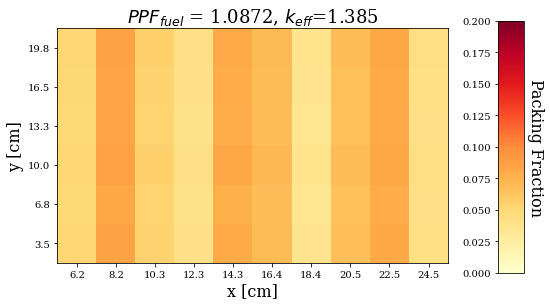
\includegraphics[width=0.49\linewidth]{a-1c-ppf-triso-comparison-most-minimized.png} 
    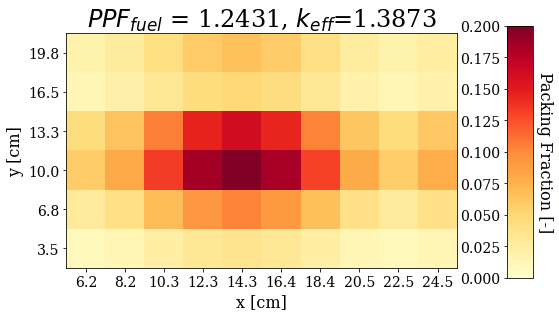
\includegraphics[width=0.49\linewidth]{a-1c-ppf-triso-comparison-least-minimized.png} 
    \caption{Simulation a-1c's most-minimized $PPF_{fuel}$ TRISO distribution 
    from Figure \ref{fig:assem-obj-1-ppf} (left) and the highest $PPF_{fuel}$ TRISO 
    distribution (right).}
    \label{fig:a-1c-ppf-triso-comparison}
\end{figure}

Figure \ref{fig:a-1c-flux-comparison} compares the 4 energy group flux distributions 
between simulation a-1c's most-minimized $PPF_{fuel}$ TRISO distribution and highest 
$PPF_{fuel}$ TRISO distribution (both shown in Figure \ref{fig:a-1c-ppf-triso-comparison}). 
\begin{figure}[htbp!]
    \centering
    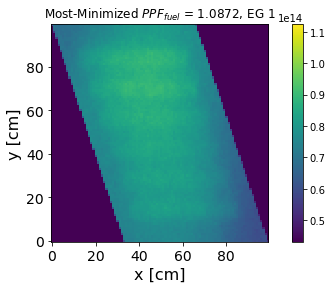
\includegraphics[width=0.35\linewidth]{flux-comparison-a-1c-most-minimized-grp1.png} 
    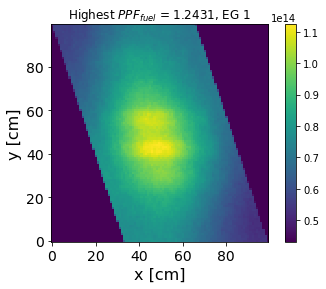
\includegraphics[width=0.35\linewidth]{flux-comparison-a-1c-least-minimized-grp1.png} 
    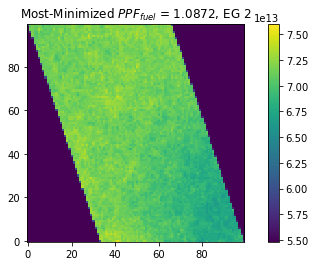
\includegraphics[width=0.35\linewidth]{flux-comparison-a-1c-most-minimized-grp2.png} 
    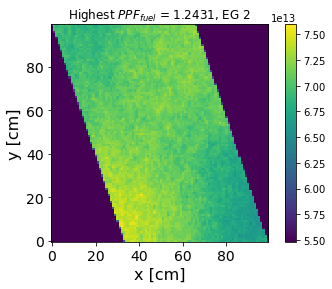
\includegraphics[width=0.35\linewidth]{flux-comparison-a-1c-least-minimized-grp2.png} 
    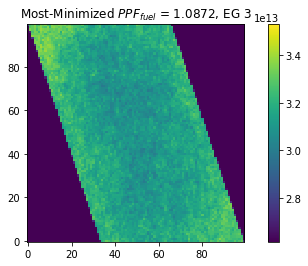
\includegraphics[width=0.35\linewidth]{flux-comparison-a-1c-most-minimized-grp3.png} 
    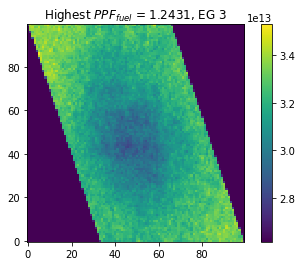
\includegraphics[width=0.35\linewidth]{flux-comparison-a-1c-least-minimized-grp3.png} 
    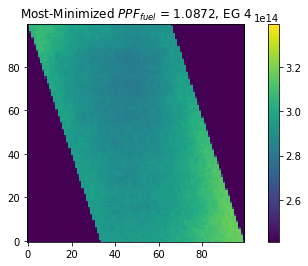
\includegraphics[width=0.35\linewidth]{flux-comparison-a-1c-most-minimized-grp4.png} 
    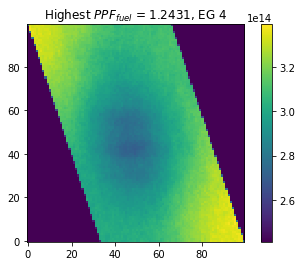
\includegraphics[width=0.35\linewidth]{flux-comparison-a-1c-least-minimized-grp4.png} 
    \caption{AHTR one-third assembly's flux comparison between the two reactor models 
    in Figure \ref{fig:a-1c-ppf-triso-comparison}: simulation a-1c's most-minimized 
    $PPF_{fuel}$ reactor model with $PPF_{fuel} = 1.0872$ and simulation a-1c's reactor 
    model with the highest $PPF_{fuel} = 1.2431$.
    Energy Group 1: E $> 9.1188 \times 10^{-3}$ MeV, 
    Energy Group 2: $2.9023 \times 10^{-5} < E < 9.1188 \times 10^{-3}$ MeV,
    Energy Group 3:  $1.8556 \times 10^{-5} < E < 2.9023 \times 10^{-5}$ MeV,
    Energy Group 4:  $1.0 \times 10^{-12} < E < 1.8554 \times 10^{-6}$ MeV.}
    \label{fig:a-1c-flux-comparison}
\end{figure}
% todo: add units... 
In Figure \ref{fig:a-1c-flux-comparison}, the reactor model with the highest 
$PPF_{fuel}$'s Group 4 flux dips in the center of the one-third assembly likely
due to spatial self-shielding effects. 
In the highest $PPF_{fuel}$ reactor model's Group 1 flux, there is a peak in 
fast neutrons born in the one-third assembly's center, the fast neutrons are 
moderated in the graphite matrix and graphite structure.
The self-shielding neutrons are more likely absorbed at the fuel regions at the 
one-third assembly's top, bottom, and sides, near the pure graphite structure 
moderating regions. 
The outer sides of the one-third assembly absorb these neutrons and geometrically 
shield the one-third assembly's center from neutron flux, leading to a relatively 
lower group 4 thermal flux in the center. 

Table \ref{tab:a-1c-flux-comparison} quantifies the total flux differences per energy 
group between the reactor models. 
I used a 100 x 100 mesh to tally the flux values for each energy group within the 
one-third assembly model.
\begin{table}[htbp!]
    \centering
    \onehalfspacing
    \caption{Flux value comparison between the two reactor models in Figure 
    \ref{fig:a-1c-ppf-triso-comparison}: simulation a-1c's most-minimized $PPF_{fuel}$ reactor model 
    with $PPF_{fuel} = 1.0872$ and simulation a-1c's reactor model with the highest 
    $PPF_{fuel} = 1.2431$.
    Energy Group 1: E $> 9.1188 \times 10^{-3}$ MeV, 
    Energy Group 2: $2.9023 \times 10^{-5} < E < 9.1188 \times 10^{-3}$ MeV,
    Energy Group 3:  $1.8556 \times 10^{-5} < E < 2.9023 \times 10^{-5}$ MeV,
    Energy Group 4:  $1.0 \times 10^{-12} < E < 1.8554 \times 10^{-6}$ MeV.}
	\label{tab:a-1c-flux-comparison}
    \footnotesize
    \begin{tabular}{lp{4cm}p{4cm}p{3cm}}
    \hline
    \textbf{Energy Group} &
    \textbf{$max(\phi)/min(\phi)$ Most-minimized $PPF_{fuel}$ TRISO Distribution} & 
    \textbf{$max(\phi)/min(\phi)$ Highest $PPF_{fuel}$ TRISO Distribution} & 
    \textbf{$\%$ Difference}\\
    \hline 
    1 & 1.825 & 2.608 & \Minus30.00 \\
    2 & 1.341 & 1.386 & \Minus3.18 \\
    3 & 1.302 & 1.334 & \Minus2.43 \\
    4 & 1.319 & 1.331 & \Minus0.85 \\
    \hline
    \end{tabular}
\end{table}
In energy group 4, the most-minimized $PPF_{fuel}$ flux distribution is $0.85\%$ flatter 
than the reactor model with the highest $PPF_{fuel} = 1.2431$.
These results verify that, similar to the \gls{AHTR} plank model, the \gls{AHTR} one-third 
assembly model's minimize $PPF_{fuel}$ objective is also driven by flattening thermal 
(Group 4) flux distribution since $max(\Phi_j) \div ave(\Phi_j) \propto PPF_{fuel}$
(Equation \ref{eq:flux-prop-ppf}). 

\paragraph{Simulation p-1f}
In Section \ref{sec:assem-1-obj-ppf}'s simulation a-1f, I conducted a single-objective 
optimization simulation to minimize fuel-normalized power peaking factor ($PPF_{fuel}$) by 
varying coolant channel shape. 
In simulation a-1f, \gls{ROLLO} found no correlation between $PPF_{fuel}$ and coolant 
channel shape (demonstrated in Figure \ref{fig:a-1f}). 

\paragraph{Summary}
I verified that the minimize $PPF_{fuel}$ objective for the \gls{AHTR} one-third 
assembly model is also driven by flattening thermal (Group 4) flux distribution and,
by extension, the fission distribution in the fuel. 
The minimize $PPF_{fuel}$ objective influences $PF_{total}$ and oscillations in the 
TRISO distribution.
The objective does not correlate with the coolant channel shape.

\subsection{Single-Objective Optimization Major Takeaways}
Section \ref{sec:assem-one-obj} utilizes the \gls{AHTR} plank 
characterizations in Chapter \ref{chap:ahtr-plank-opt-results} to conduct
a comparative analysis to verify if the same driving factors apply to the 
\gls{AHTR} one-third assembly model's optimization objectives. 
In Section \ref{sec:assem-one-obj}'s single-objective optimization simulations: 
a-1a, a-1b, a-1c, a-1d, a-1e, a-1f; and Section \ref{sec:assem-discussion-single}'s 
discussions, I verified that each of the one-third assembly objective follows the 
same driving factors as the \gls{AHTR} plank optimization objectives and described 
each objective's relationship with each input parameter. 
I determined that \gls{ROLLO} flattens TRISO distribution and maximizes the coolant 
channel shape's radius values ($r_1, r_2, r_3, r_4, r_5$) that are located close to 
the reactor model's temperature peak to achieve the minimize $T_{max}$ objective. 
The minimize $PF_{total}$ objective is driven by maximizing the one-third assembly's 
total fission reaction rate and influences oscillations in the TRISO distribution to 
achieve the objective. 
The minimize $PPF_{fuel}$ objective is driven by flattening the one-third assembly's 
thermal flux distribution and influences $PF_{total}$ and oscillations in the TRISO 
distribution to achieve the objective. 
Both the minimize $PF_{total}$ and minimize $PPF_{fuel}$ objectives do not correlate
with the coolant channel shape. 
Simulation a-1b and a-1e results demonstrated that coolant channel shape variation 
does not have as high of an impact on $T_{max}$ as \gls{TRISO} distribution variation.
Since the variations in coolant channel shape only impact the minimize maximum 
temperature ($T_{max}$) objective, I do not conduct double-objective 
optimization for coolant channel shape variations.  

\section{AHTR One-Third Assembly: Double-Objective Optimization Results}
\label{sec:assem-two-obj}
This section reports the \gls{AHTR} one-third assembly's \gls{ROLLO} double-objective 
optimization results. 
The previous section's single-objective optimization results inform the double-objective 
optimization simulations in this section.
Section \ref{sec:assem-one-obj} concluded that coolant channel shape variations 
only correlate with the minimize $T_{max}$ objective, thus, I do not conduct 
double-objective optimization for coolant channel shape variations.
I run double-objective optimization simulations that vary total fuel packing 
fraction ($PF_{total}$) and \gls{TRISO} packing fraction distribution 
($\rho_{TRISO}(\vec{r})$), for combinations of the three objectives (minimize 
$PF_{total}$, $T_{max}$, and $PPF_{fuel}$). 
Earlier in this chapter, Table \ref{tab:assem-obj-breakdown} summarized the 
double-objective simulations: a-2a, a-2b, and a-2c.

As described in Section \ref{sec:opt}, multi-objective optimization returns 
multiple optimal solutions that meet each objective to varying degrees; this set of 
solutions is the Pareto front \cite{deb_multi-objective_2001}. 
For each solution in the Pareto front, none of the objective functions can be 
improved without degrading another objective.
An ideal optimization method for a multi-objective problem like reactor design 
optimization should find widely spread out reactor model solutions in the Pareto front 
\cite{deb_multi-objective_2001}. 
Thus, I report on the optimal reactor models on the Pareto front for the 
multi-objective optimization problems in this section and Section 
\ref{sec:assem-three-obj}. 
Several optimal solutions will be highlighted in the Pareto front figures. 

To ensure that the multi-objective optimization problems are converged, I report the 
hypervolume values for each generation. 
As previously described in Section \ref{sec:binhandkorn}, the hypervolume indicator 
quantifies the Pareto front's goodness (bigger = better).
The hypervolume is calculated by finding the volume between the reference point and 
the objective values of the Pareto front's reactor models. 
The reference point must be selected to ensure that every reactor model falls within 
the hypervolume; thus, I use a different reference point for each optimization problem.
I use the hypervolume values to determine if the simulation converges across generations 
and do not compare them across different optimization simulations.
The hypervolume is converging if the difference between generations' hypervolume values 
is getting smaller. 

For a single generation with 128 reactor models, OpenMC and Moltres software must be 
run for each reactor model, resulting in high computational cost. 
For each optimization simulation, I must balance convergence and computational cost.
\gls{ROLLO}'s purpose is to help the human reactor designer narrow down reactor design 
the search space, therefore, the reactor designer uses the computational 
power available to them, to narrow down the search space as much as possible. 
Section \ref{sec:rollo-convergence} described that the reactor designer should 
plot the Pareto front and observe the hypervolume values to evaluate if they are 
confident about the final solution set.  
Thus, I determine if convergence criteria is met by evaluating if the difference 
between generations' hypervolume values are getting smaller. 
If a multi-objective optimization problem's hypervolume converges earlier than the 
five generations I intended to run (determined in Section 
\ref{sec:multi-obj-hyperparameters}), I stop the simulation at that generation. 
However, if the multi-objective optimization problem's hypervolume does not converge by 
generation 5, I run the problem for a few more generations until satisfactory 
convergence is achieved.

\subsection{a-2a: Minimize $PF_{total}$ and $T_{max}$}
\label{sec:a-2a}
This section reports results from the double-objective optimization simulation a-2a; the 
objectives minimized are total fuel packing fraction ($PF_{total}$) and maximum
temperature ($T_{max}$).  
Table \ref{tab:simulationa2a} summarizes simulation a-2a's optimization problem parameters. 
\begin{table}[htbp!]
    \centering
    \onehalfspacing
    \caption{Simulation a-2a Optimization Problem Parameters}
	\label{tab:simulationa2a}
    \footnotesize
    \begin{tabular}{l|p{5.3cm}}
    \hline 
    \multicolumn{2}{c}{\textbf{Two Objectives: Simulation a-2a}} \\
    \hline 
    \textbf{Objectives} & Minimize $PF_{total}$ \\
    & Minimize $T_{max}$ \\
    \hline 
    \textbf{Input parameter variations} & $0.05 \leq PF_{total} \leq 0.07$ \\
    & $\rho_{TRISO}(\vec{r})$: $0 \leq a \leq 2$, $0 \leq d \leq 2$\\
    & $\rho_{TRISO}(\vec{r})$: $0 \leq b \leq \frac{\pi}{2}$, $0 \leq e \leq \frac{\pi}{2}$\\
    & $\rho_{TRISO}(\vec{r})$: $0 \leq c \leq 2\pi$, $0 \leq f \leq 2\pi$\\
    \hline
    \textbf{Constraints} & $k_{eff} \geq 1.38$\\ 
    \hline 
    \textbf{Genetic algorithm parameters} & Population size: 128 \\
    & Generations: 5 \\
    \hline
    \end{tabular}
\end{table}
Table \ref{tab:a2a-hypervolume} shows the hypervolume value at each generation, 
confirming that simulation a-2a converges by generation 5. 
\begin{table}[htbp!]
    \centering
    \onehalfspacing
    \caption{Simulation a-2a hypervolume values at each generation.}
	\label{tab:a2a-hypervolume}
    \footnotesize
    \begin{tabular}{ll}
    \hline 
    \multicolumn{2}{c}{\textbf{Two Objectives: Simulation a-2a}} \\
    \multicolumn{2}{c}{Reference point: (0.07, 1700)} \\
    \hline 
    \textbf{Generation} & \textbf{Hypervolume [-]} \\
    \hline
    1 & 6.0090 \\
    2 & 6.0859 \\
    3 & 6.2220 \\
    4 & 6.3379 \\
    5 & 6.4664 \\
    \hline
    \end{tabular}
\end{table}

Figure \ref{fig:assem-obj-2-pftemp-pareto} shows a plot of the final generation's 
reactor models' $PF_{total}$ against $T_{max}$; crosses mark the reactor models 
that fall on the Pareto front.
Figure \ref{fig:assem-obj-2-pftemp-pareto-distr} shows the 22 TRISO packing fraction 
distributions in the final generation, labeled numerically, that fall on the 
Pareto front. 
\begin{figure}[htbp!]
    \begin{subfigure}{\textwidth}
        \centering
        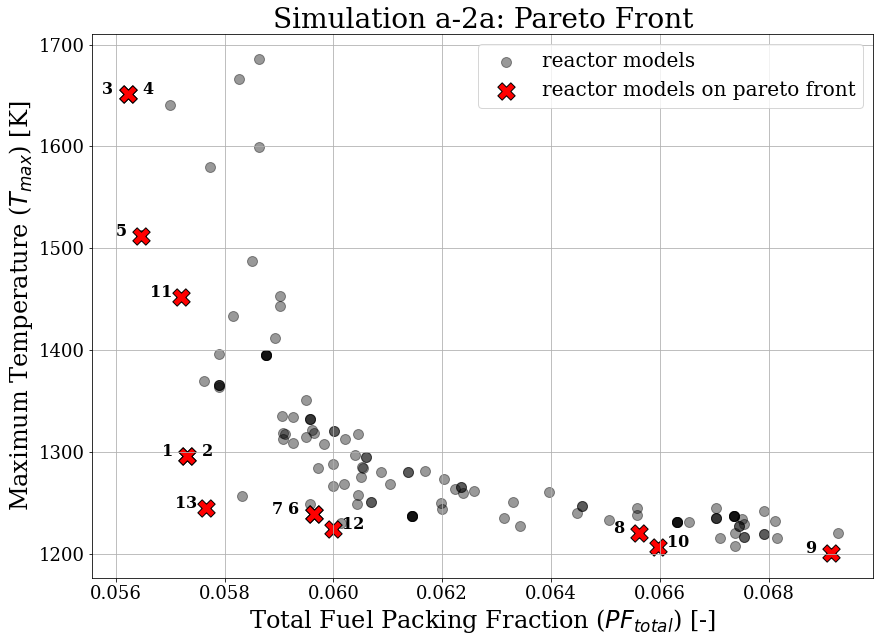
\includegraphics[width=\linewidth]{assem-obj-2-pftemp-pareto.png}
        \caption{Plot of final generation's reactor models' $PF_{total}$ against 
        $T_{max}$. 
        Crosses indicate the reactor models on the Pareto front. Annotated numbers 
        on each cross correspond to TRISO distributions in the plot below.}
        \label{fig:assem-obj-2-pftemp-pareto} 
    \end{subfigure}
    \caption{Simulation a-2a -- ROLLO double-objective optimization to minimize total fuel 
    packing fraction ($PF_{total}$) and maximum temperature ($T_{max}$) in 
    the one-third assembly. 
    Input parameters varied: total fuel packing fraction ($PF_{total}$) and TRISO 
    packing fraction distribution ($\rho_{TRISO}(\vec{r})$).}
    \label{fig:assem-obj-2-pftemp}
\end{figure}
\begin{figure}[htbp!]
    \ContinuedFloat
    \begin{subfigure}{\textwidth}
        \centering
        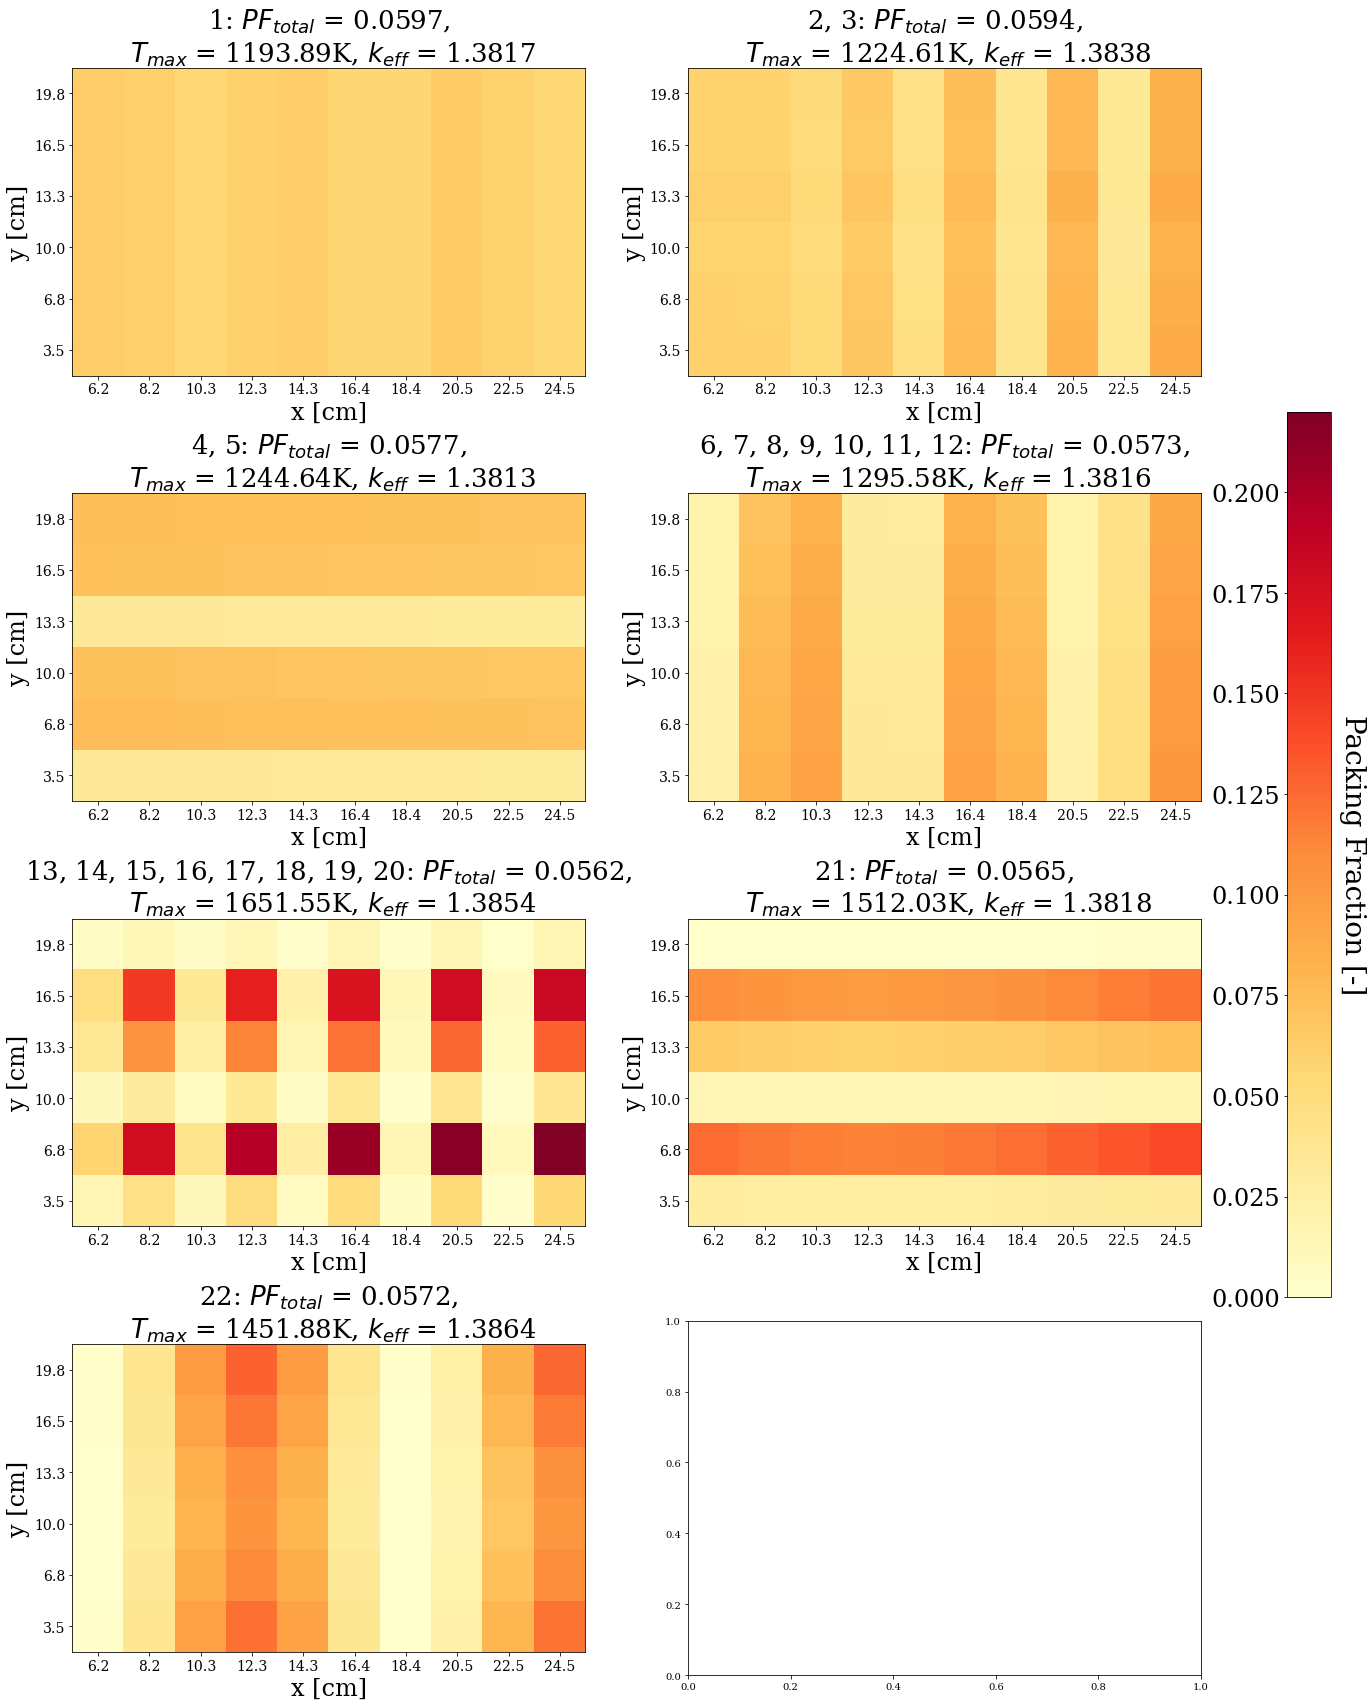
\includegraphics[width=0.95\linewidth]{assem-obj-2-pftemp-pareto-distr.png}
        \caption{TRISO distribution for the 22 reactor models on the Pareto front.
        Numbered reactor models correspond to numbered crosses in the plot above. 
        Note that some models have identical distributions, resulting in the 7 plots in 
        this subfigure.}
        \label{fig:assem-obj-2-pftemp-pareto-distr} 
    \end{subfigure}
    \caption{(contd.) Simulation a-2a -- ROLLO double-objective optimization to minimize total fuel 
    packing fraction ($PF_{total}$) and maximum temperature ($T_{max}$) in 
    the one-third assembly. 
    Input parameters varied: total fuel packing fraction ($PF_{total}$) and TRISO 
    packing fraction distribution ($\rho_{TRISO}(\vec{r})$).}
\end{figure}

Figure \ref{fig:assem-obj-2-pftemp-pareto} shows that minimize $PF_{total}$ and 
minimize $T_{max}$ are competing objectives. 
That is, by minimizing $T_{max}$ we increase $PF_{total}$ and by minimizing 
$PF_{total}$ we increase $T_{max}$. 
In Figure \ref{fig:assem-obj-2-pftemp}, the one-third assembly model with the 
most-minimized $PF_{total}$ and highest $T_{max}$ are reactor models 13 to 20. 
These models have an oscillating TRISO distribution along the 
x-axis and y-axis, and a packing fraction standard deviation of $0.066$ across the 
one-third assembly. 
Along the x-axis, the distribution peaks at the even fuel cell columns (at 8.2cm,  
and 12.3cm, 16.4cm, 20.5cm, and 24.5cm) and has minimum points at the odd fuel cell 
columns (at 6.2cm, 10.3cm, 14.3cm, 18.4cm, and 22.5cm).
The even fuel cell columns have a ${\sim}0.18$ y-axis variation with peaks of 
$PF\approx0.21$. 

In Figure \ref{fig:assem-obj-2-pftemp}, the one-third assembly model with the 
most-minimized $T_{max}$ and highest $PF_{total}$ is reactor model 1. 
Reactor model 1 has an almost constant TRISO packing fraction distribution with 
a packing fraction standard deviation of $0.004$ across the one-third assembly. 
The one-third assembly model that minimizes both $PF_{total}$ and $T_{max}$ 
to an equal extent based on visual inspection of the Pareto Front (Figure 
\ref{fig:assem-obj-2-pftemp-pareto}) are reactor models 4 and 5. 
Reactor models 4 and 5 have an oscillating TRISO distribution along the y-axis and 
a packing fraction standard deviation of $0.018$ across the one-third assembly. 
Along the y-axis, the distribution peaks at the 2nd, 3rd, 5th, and 6th rows 
(at 6.8cm, 10.0cm, 16.5cm, and 19.8cm) with $PF\approx0.07$ and has minimum points at 
the 1st and 4th rows (at 3.5cm and 13.3cm) with $PF\approx0.03$. 
Section \ref{sec:assem-discussion-multi} discusses and explains simulation a-2a's 
results.

\subsection{a-2b: Minimize $PF_{total}$ and $PPF_{fuel}$}
\label{sec:a-2b}
This section reports results from the double-objective optimization simulation a-2b; the 
objectives minimized are total fuel packing fraction ($PF_{total}$) and fuel-normalized 
power peaking factor ($PPF_{fuel}$) in the one-third assembly.  
Table \ref{tab:simulationa2b} summarizes simulation a-2b's optimization problem parameters. 
\begin{table}[htbp!]
    \centering
    \onehalfspacing
    \caption{Simulation a-2b Optimization Problem Parameters}
	\label{tab:simulationa2b}
    \footnotesize
    \begin{tabular}{l|p{5.3cm}}
    \hline 
    \multicolumn{2}{c}{\textbf{Two Objectives: Simulation a-2b}} \\
    \hline 
    \textbf{Objectives} & Minimize $PF_{total}$ \\
    & Minimize $PPF_{fuel}$ \\
    \hline 
    \textbf{Input parameter variations} & $0.05 \leq PF_{total} \leq 0.07$ \\
    & $\rho_{TRISO}(\vec{r})$: $0 \leq a \leq 2$, $0 \leq d \leq 2$\\
    & $\rho_{TRISO}(\vec{r})$: $0 \leq b \leq \frac{\pi}{2}$, $0 \leq e \leq \frac{\pi}{2}$\\
    & $\rho_{TRISO}(\vec{r})$: $0 \leq c \leq 2\pi$, $0 \leq f \leq 2\pi$\\
    \hline
    \textbf{Constraints} & $k_{eff} \geq 1.38$\\ 
    \hline 
    \textbf{Genetic algorithm parameters} & Population size: 128 \\
    & Generations: 5 \\
    \hline
    \end{tabular}
\end{table}
Table \ref{tab:a2b-hypervolume} shows the hypervolume value at each generation, 
confirming that simulation a-2b converges by generation 5. 
\begin{table}[htbp!]
    \centering
    \onehalfspacing
    \caption{Simulation a-2b hypervolume values at each generation.}
	\label{tab:a2b-hypervolume}
    \footnotesize
    \begin{tabular}{ll}
    \hline 
    \multicolumn{2}{c}{\textbf{Two Objectives: Simulation a-2b}} \\
    \multicolumn{2}{c}{Reference point: (0.07, 1.9)} \\
    \hline 
    \textbf{Generation} & \textbf{Hypervolume [-]} \\
    \hline
    1 & 0.00989 \\
    2 & 0.00991 \\
    3 & 0.00997 \\
    4 & 0.01054\\
    5 & 0.01058\\
    \hline
    \end{tabular}
\end{table}

Figure \ref{fig:assem-obj-2-pfppf-pareto} shows a plot of the final generation's reactor 
models' $PF_{total}$ against $PPF_{fuel}$; crosses mark the reactor models that fall on 
the Pareto front.
Figure \ref{fig:assem-obj-2-pfppf-pareto-distr} shows the 12 TRISO packing fraction 
distributions, labeled numerically, that fall on the Pareto front. 
\begin{figure}[htbp!]
    \begin{subfigure}{\textwidth}
        \centering
        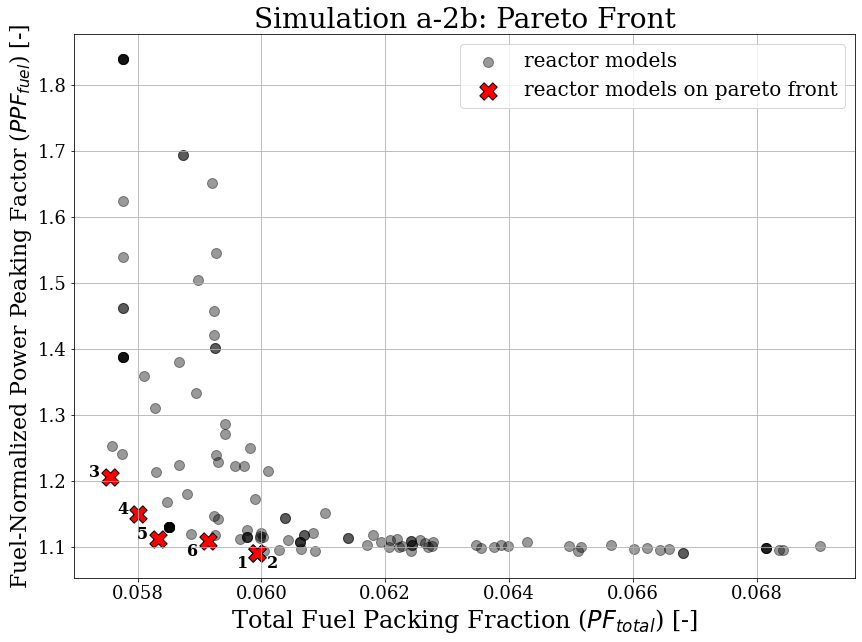
\includegraphics[width=\linewidth]{assem-obj-2-pfppf-pareto.png}
        \caption{Plot of final generation's reactor models' $PF_{total}$ against 
        $PPF_{fuel}$. 
        Crosses indicate the reactor models on the Pareto front. Annotated numbers 
        on each cross correspond to TRISO distributions in Figure 
        \ref{fig:assem-obj-2-pfppf-pareto-distr}.}
        \label{fig:assem-obj-2-pfppf-pareto} 
    \end{subfigure}
    \caption{Simulation a-2b -- ROLLO double-objective optimization to minimize total fuel 
    packing fraction ($PF_{total}$) and normalized power peaking factor ($PPF_{fuel}$) 
    in the \gls{AHTR} one-third assembly. 
    Input parameters varied: $PF_{total}$ and TRISO 
    packing fraction distribution ($\rho_{TRISO}(\vec{r})$).}
    \label{fig:assem-obj-2-pfppf}
\end{figure}
\begin{figure}[htbp!]
    \ContinuedFloat
    \begin{subfigure}{\textwidth}
        \centering
        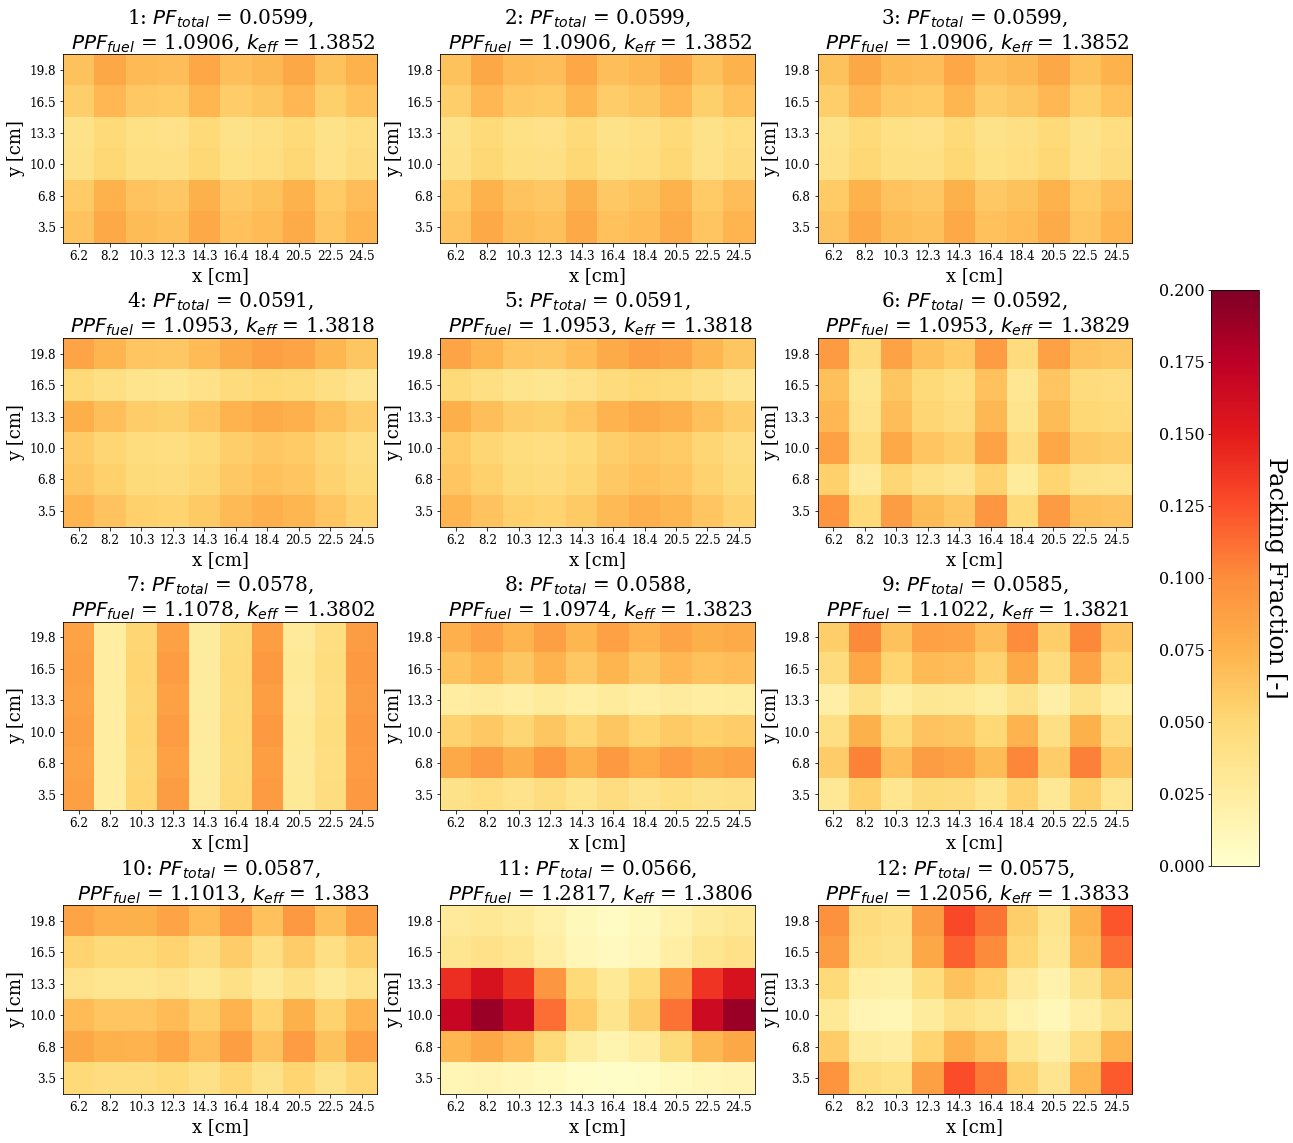
\includegraphics[width=\linewidth]{assem-obj-2-pfppf-pareto-distr.png}
        \caption{TRISO distribution for the 12 reactor models on the Pareto front.
        Numbered reactor models correspond to numbered crosses in Figure 
        \ref{fig:assem-obj-2-pfppf-pareto}. Note that some models have identical 
        distributions, resulting in the 9 plots in this subfigure.}
        \label{fig:assem-obj-2-pfppf-pareto-distr} 
    \end{subfigure}
    \caption{(contd.) Simulation a-2b -- ROLLO double-objective optimization to minimize total fuel 
    packing fraction ($PF_{total}$) and normalized power peaking factor ($PPF_{fuel}$) 
    in the \gls{AHTR} one-third assembly. 
    Input parameters varied: $PF_{total}$ and TRISO 
    packing fraction distribution ($\rho_{TRISO}(\vec{r})$).}
\end{figure}

Figure \ref{fig:assem-obj-2-pfppf-pareto} shows that minimize $PF_{total}$ and 
minimize $PPF_{fuel}$ are competing objectives. 
In Figure \ref{fig:assem-obj-2-pfppf}, the one-third assembly model with 
the most-minimized $PF_{total}$ and highest $PPF_{fuel}$ is reactor model 11. 
Reactor model 11 has an oscillating TRISO distribution along the 
x-axis and y-axis, and a packing fraction standard deviation of $0.053$ across the 
one-third assembly. 
Along the y-axis, the distribution peaks at the 3rd and 4th fuel cell rows (at 
10.0cm amd 13.3cm) and has minimum points at the 1st, 5th, and 6th fuel cell rows 
(at 3.5cm, 16.5cm, 19.8cm). 
The 3rd and 4th rows have the largest x-axis variation of ${\sim}0.14$ with 
peaks of $PF\approx0.17$. 
The 1st, 5th, and 6th row has the smallest x-axis variation of ${\sim}0.02$ with 
minimums of $PF\approx0.005$. 

In Figure \ref{fig:assem-obj-2-pfppf}, the one-third assembly model with 
the most-minimized $PPF_{fuel}$ and highest $PF_{total}$ is reactor model 1.
Reactor model 1 has an oscillating TRISO distribution along the 
x-axis and y-axis and a packing fraction standard deviation of $0.013$ across the 
one-third assembly.
Along the x-axis, the distribution peaks at the 2nd, 5th, and 8th fuel cell columns (at 
8.2cm, 14.3cm, and 20.5cm) and has minimum points at the 1st, 6th, and 9th (at 6.2cm, 
16.4cm, and 22.5cm).
The 2nd, 5th, and 8th columns have the largest y-axis variation of ${\sim}0.034$ with 
peaks of $PF\approx0.08$.
The 1st, 6th, and 9th columns have the smallest y-axis variation of ${\sim}0.027$ with 
minimums of $PF\approx0.038$. 
On the y-axis, the distribution has peaks at the top and bottom row (at 3.5cm and 
19.8cm) and has a minimum point in the center rows (at 10.0cm and 13.3cm).
The top and bottom row have the largest x-axis variation of ${\sim}0.018$ with 
peaks of $PF\approx0.08$.
The center rows have the smallest x-axis variation of ${\sim}0.011$ with minimums 
of $PF\approx0.038$. 

The one-third assembly model that minimizes both $PF_{total}$ and $PPF_{fuel}$ 
to an equal extent based on visual inspection of the Pareto Front (Figure 
\ref{fig:assem-obj-2-pfppf-pareto}) is reactor model 5. 
Like reactor models 11 and 1, reactor model 5 has an oscillating TRISO 
distribution along the x-axis and y-axis. 
Reactor model 5 has a packing fraction standard deviation of $0.013$ across the 
one-third assembly.
Along the x-axis, the distribution peaks at the 1st and 7th fuel cell columns 
(at 6.2cm and 18.4cm) and has minimum points in the 3rd, 4th, and 10th fuel cell 
columns (at 10.3cm, 12.3cm, and 24.5cm).
Along the x-axis, all the columns have a similar x-axis variation of ${\sim}0.03$.
Along the y-axis, the distribution peaks at the 4th and 6th fuel cell rows (at 13.3cm 
and 19.8cm) and has minimum points at the 5th fuel row (at 16.5cm). 
The 4th and 6th rows have the largest x-axis variation of ${\sim}0.024$ with peaks of 
$PF\approx0.08$. 
The 5th row has the smallest x-axis variation of ${\sim}0.015$ with minimums of 
$PF\approx0.035$. 
Sections \ref{sec:assem-discussion-multi} discusses and explains simulation a-2b's 
results.

\subsection{a-2c: Minimize $T_{max}$ and $PPF_{fuel}$}
\label{sec:a-2c}
This section reports results from the double-objective optimization simulation a-2c; 
minimized objectives are maximum temperature ($T_{max}$) and fuel-normalized power 
peaking factor ($PPF_{fuel}$) in the one-third assembly.  
Table \ref{tab:simulationa2c} summarizes simulation a-2c's optimization problem parameters. 
\begin{table}[htbp!]
    \centering
    \onehalfspacing
    \caption{Simulation a-2c Optimization Problem Parameters}
	\label{tab:simulationa2c}
    \footnotesize
    \begin{tabular}{l|p{5.3cm}}
    \hline 
    \multicolumn{2}{c}{\textbf{Two Objectives: Simulation a-2c}} \\
    \hline 
    \textbf{Objectives} & Minimize $T_{max}$ \\
    & Minimize $PPF_{fuel}$ \\
    \hline 
    \textbf{Input parameter variations}
    & $\rho_{TRISO}(\vec{r})$: $0 \leq a \leq 2$, $0 \leq d \leq 2$\\
    & $\rho_{TRISO}(\vec{r})$: $0 \leq b \leq \frac{\pi}{2}$, $0 \leq e \leq \frac{\pi}{2}$\\
    & $\rho_{TRISO}(\vec{r})$: $0 \leq c \leq 2\pi$, $0 \leq f \leq 2\pi$\\
    \hline
    \textbf{Constraints} & $k_{eff} \geq 1.38$\\ 
    & $PF_{total} = 0.06$\\
    \hline 
    \textbf{Genetic algorithm parameters} & Population size: 128 \\
    & Generations: 2 \\
    \hline
    \end{tabular}
\end{table}
Table \ref{tab:a2c-hypervolume} shows the hypervolume value at each generation, 
confirming that simulation a-2c converges by generation 2. 
\begin{table}[htbp!]
    \centering
    \onehalfspacing
    \caption{Simulation a-2c hypervolume values at each generation.}
	\label{tab:a2c-hypervolume}
    \footnotesize
    \begin{tabular}{ll}
    \hline 
    \multicolumn{2}{c}{\textbf{Two Objectives: Simulation a-2c}} \\
    \multicolumn{2}{c}{Reference point: (1700, 1.5)} \\
    \hline 
    \textbf{Generation} & \textbf{Hypervolume [-]} \\
    \hline
    1 & 210.685 \\
    2 & 210.685 \\
    \hline
    \end{tabular}
\end{table}

Figure \ref{fig:assem-obj-2-tempppf-pareto} shows a plot of the final generation's 
reactor models' $T_{max}$ against $PPF_{fuel}$; crosses mark the reactor models 
that fall on the Pareto front.
% todo: comment on the shape of this pareto front. is it even a front? 
Figure \ref{fig:assem-obj-2-tempppf-pareto-distr} shows the one TRISO packing fraction 
distribution in the final generation that falls on the Pareto front. 
Figure \ref{fig:assem-obj-2-tempppf-min-tempppf} illustrates the one \gls{AHTR} one-third 
assembly model on the Pareto front. 
\begin{figure}[htbp!]
    \centering
    \begin{subfigure}{\textwidth}
        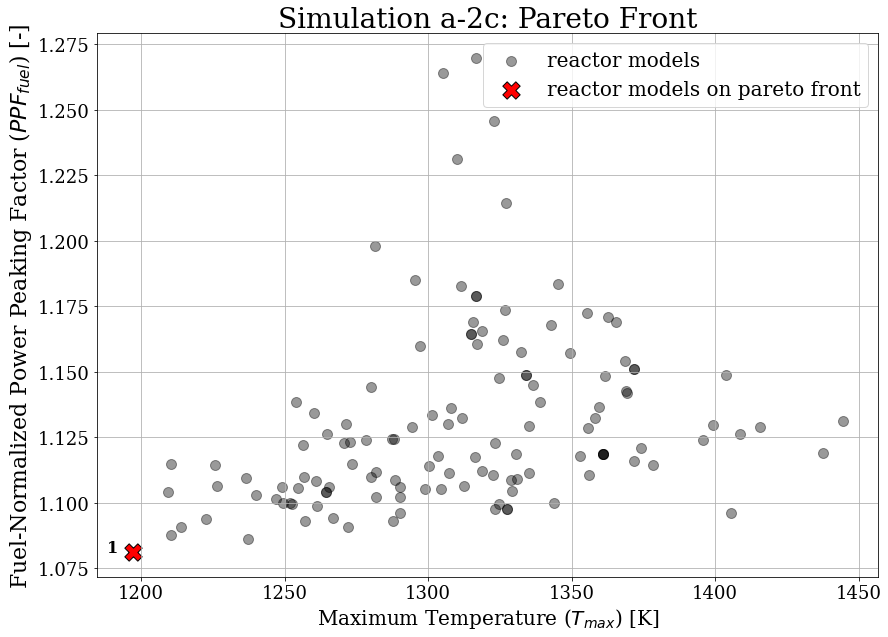
\includegraphics[width=\linewidth]{assem-obj-2-tempppf-pareto.png}
        \caption{Plot of final generation's reactor models' $T_{max}$ against 
        $PPF_{fuel}$. 
        Crosses indicate the reactor models on the Pareto front. Annotated numbers 
        on each cross correspond to TRISO distributions in the plot below.}
        \label{fig:assem-obj-2-tempppf-pareto} 
    \end{subfigure}
    \caption{Simulation a-2c -- ROLLO double-objective optimization to minimize 
    one-third assembly's maximum temperature ($T_{max}$) and fuel-normalized power peaking factor 
    ($PPF_{fuel}$) in the \gls{AHTR} one-third assembly. 
    Input parameters varied: TRISO packing fraction distribution ($\rho_{TRISO}(\vec{r})$).}
    \label{fig:assem-obj-2-tempppf}
\end{figure}
\begin{figure}[htbp!]
    \ContinuedFloat
    \begin{subfigure}{\textwidth}
        \centering
        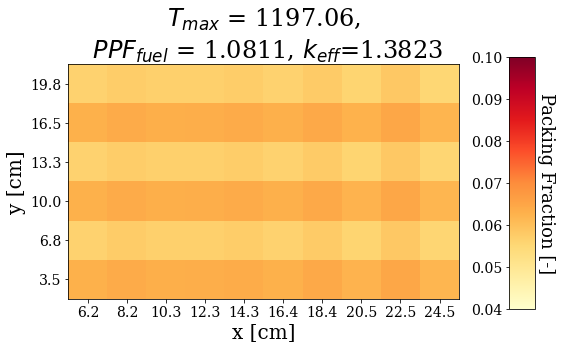
\includegraphics[width=0.7\linewidth]{a-2c-most-minimized.png}
        \caption{TRISO distribution for the 1 reactor model on the Pareto front.
        Numbered reactor models correspond to numbered crosses in the plot above. }
        \label{fig:assem-obj-2-tempppf-pareto-distr} 
    \end{subfigure}
    \begin{subfigure}{\textwidth}
        \centering
        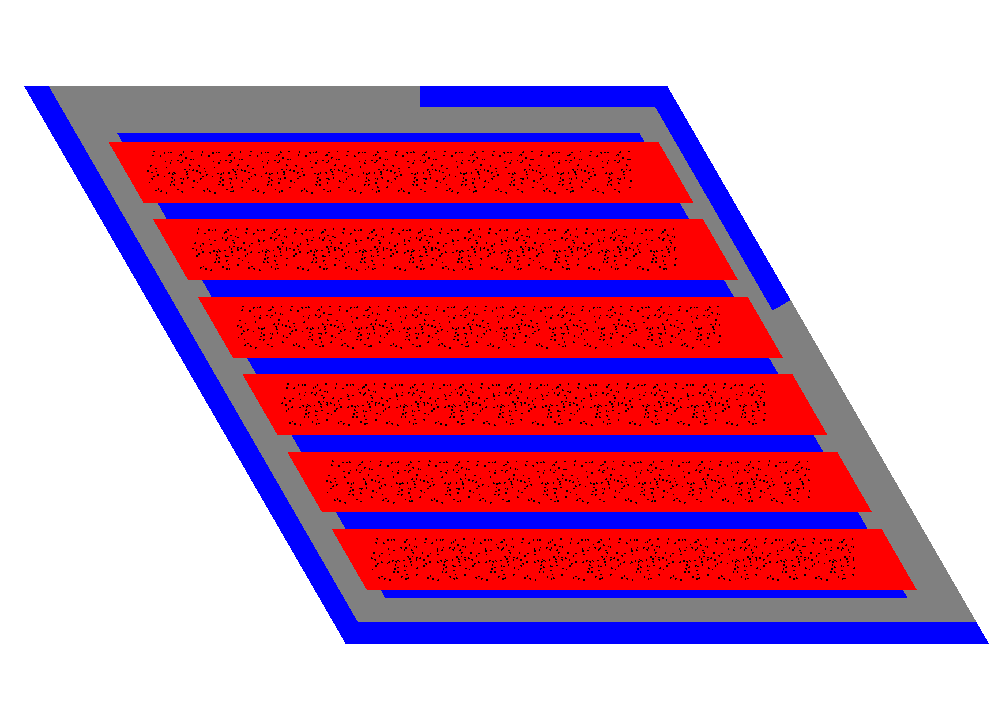
\includegraphics[width=0.7\linewidth]{assem-obj-2-tempppf-min-both.png}
        \caption{\gls{AHTR} one-third assembly model with the most-minimized $T_{max}$ and 
        $PPF_{fuel}$ (corresponds to the TRISO distribution in the above plot).}
        \label{fig:assem-obj-2-tempppf-min-tempppf} 
    \end{subfigure}
    \caption{(contd.) Simulation a-2c -- ROLLO double-objective optimization to minimize 
    one-third assembly's maximum temperature ($T_{max}$) and fuel-normalized power peaking factor 
    ($PPF_{fuel}$) in the \gls{AHTR} one-third assembly. 
    Input parameters varied: TRISO packing fraction distribution ($\rho_{TRISO}(\vec{r})$).}
\end{figure}

Figure \ref{fig:assem-obj-2-tempppf-pareto} shows that minimize $T_{max}$ and minimize 
$PPF_{fuel}$ are non-competing objectives, resulting in a single reactor model on the 
Pareto Front. 
Figure \ref{fig:assem-obj-2-tempppf-pareto-distr} shows the TRISO distribution that best 
minimizes both $T_{max}$ and $PPF_{fuel}$. 
The reactor model has a TRISO distribution that oscillates along the y-axis and 
slightly on the x-axis, and a packing fraction standard deviation of $0.033$ 
across the one-third assembly. 
Along the y-axis, the distribution peaks at the odd rows (at 3.5cm, 10.0cm, and 16.5cm) 
with $PF\approx0.06$ and has minimum points at the even rows (at 6.8cm, 13.3cm, and 
19.8cm) with $PF\approx0.055$.
Sections \ref{sec:assem-discussion-multi} discusses and explains simulation a-2c's 
results.

\subsection{Double-Objective Optimization Discussion}
\label{sec:assem-discussion-two}
In this section, I explain how the driving factors and phenomena observed in 
the previous single-objective discussion (Section \ref{sec:assem-discussion-single}) 
combine to result in the optimal reactor models found by the double-objective 
optimization simulations. 

\subsubsection{Simulation a-2a}
In Section \ref{sec:a-2a}'s simulation a-2a, I conducted a two-objective 
optimization simulation to minimize total fuel packing fraction ($PF_{total}$) and 
maximum temperature ($T_{max}$) in a one-third assembly model by varying $PF_{total}$ 
and TRISO distribution. 
In simulation a-2a, ROLLO found 13 reactor models on the Pareto Front (Figure 
\ref{fig:assem-obj-2-pftemp-pareto}). 

In simulation a-2a, \gls{ROLLO} found that the one-third assembly models with the 
most-minimized $PF_{total}$ objective are reactor models 3 and 4 (Figure 
\ref{fig:assem-obj-2-pftemp-pareto-distr}). 
Both reactor models have an oscillating TRISO distribution along the x-axis 
and y-axis. 
Figure \ref{fig:a-2a-pf-triso-comparison} compares simulation a-2a's most-minimized 
$PF_{total}$ reactor model 3 and simulation a-1a's most-minimized $PF_{total}$ reactor 
model. 
\begin{figure}[htbp!]
    \centering
    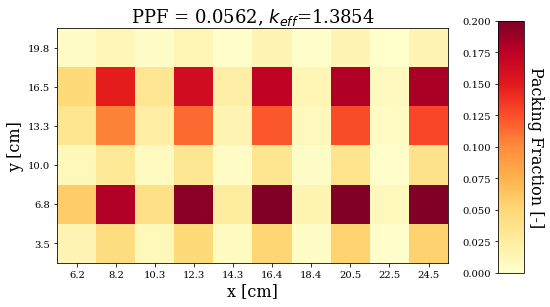
\includegraphics[width=0.49\linewidth]{a-2a-pf-most-minimized.png} 
    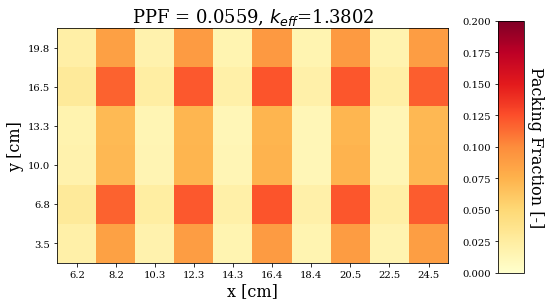
\includegraphics[width=0.49\linewidth]{assem-0.0559-most-minimized.png} 
    \caption{Simulation a-2a's most-minimized $PF_{total}$ TRISO distribution 
    from Figure \ref{fig:assem-obj-2-pftemp} (left) and simulation a-1a's 
    most-minimized $PF_{total}$ TRISO distribution from Figure 
    \ref{fig:assem-obj-1-pf} (right).}
    \label{fig:a-2a-pf-triso-comparison}
\end{figure}
Figure \ref{fig:a-2a-pf-triso-comparison} shows that simulation a-2a's most-minimized 
$PF_{total}$ reactor model, and simulation a-1a's most-minimized $PF_{total}$ reactor 
model have similar distributions with peaks on the even fuel cell columns but at 
different amplitudes. 

In simulation a-2a, \gls{ROLLO} found that the one-third assembly model with the 
most-minimized $T_{max}$ objective, reactor model 9 (Figure 
\ref{fig:assem-obj-2-pftemp-pareto-distr}), has an almost constant TRISO distribution.
Figure \ref{fig:a-2a-temp-triso-comparison} compares simulation a-2a's most-minimized 
$T_{max}$ reactor model 9 and simulation a-1b's most-minimized $T_{max}$ reactor model. 
\begin{figure}[htbp!]
    \centering
    \includegraphics[width=0.49\linewidth]{a-2a-temp-most-minimized.png} 
    \includegraphics[width=0.49\linewidth]{a-1b-temp-most-minimized.png} 
    \caption{Simulation a-2a's most-minimized $T_{max}$ TRISO distribution 
    from Figure \ref{fig:assem-obj-2-pftemp} (left) and simulation a-1b's 
    most-minimized $T_{max}$ TRISO distribution from Figure 
    \ref{fig:assem-obj-1-temp} (right).}
    \label{fig:a-2a-temp-triso-comparison}
\end{figure}
Figure \ref{fig:a-2a-temp-triso-comparison} shows that simulation a-2a's most-minimized 
$T_{max}$ reactor model, and simulation a-1b's most-minimized $T_{max}$ reactor model 
have similar, $PF_{total}$ values and almost constant TRISO distributions.
Simulation a-2a's most-minimized $T_{max}$'s TRISO distribution is not as flat 
as simulation a-1b with packing fraction standard deviations of $0.004$ and $0.0009$, 
respectively.

Figure \ref{fig:a-2a-balanced-reactor-model} shows reactor model 13, which 
minimized $PF_{total}$ and $T_{max}$ to an equal extent by balancing influences 
from both objectives. 
\begin{figure}[htbp!]
    \centering
    \includegraphics[width=0.6\linewidth]{a-2a-balanced-reactor-model.png} 
    \caption{Simulation a-2a's reactor model 13 which minimized both $PF_{total}$ and $T_{max}$ 
    to an equal extent (see Pareto Front in Figure \ref{fig:assem-obj-2-pftemp}).}
    \label{fig:a-2a-balanced-reactor-model}
\end{figure}
The \gls{TRISO} distributions on simulation a-2a's Pareto front in Figure 
\ref{fig:assem-obj-2-pftemp} minimize both $PF_{total}$ and $T_{max}$ and vary
between the two extreme cases: most-minimized $PF_{total}$ and most-minimized $T_{max}$. 
The minimize $T_{max}$ objective influences the TRISO distribution's flatness, as 
described in Section \ref{sec:assem-discussion-temp}, while 
the minimize $PF_{total}$ objective influences the oscillating pattern, as described 
in Section \ref{sec:assem-discussion-pf}.

\subsubsection{Simulation a-2b}
% compare reactor models 1,3,5's fission reaction rate and thermal flux flattness
In Section \ref{sec:a-2b}'s simulation a-2b, I conducted a two-objective 
optimization simulation to minimize total fuel packing fraction ($PF_{total}$) and 
fuel-normalized power peaking factor ($PPF_{fuel}$) in a one-third assembly model 
by varying $PF_{total}$ and TRISO packing fraction distribution. 
In simulation a-2b's final generation, ROLLO found 12 reactor models on the Pareto Front 
(Figure \ref{fig:assem-obj-2-pfppf-pareto}). 

In simulation a-2b, \gls{ROLLO} found that the one-third assembly model with the 
most-minimized $PF_{total}$ objective, reactor model 3 (Figure 
\ref{fig:assem-obj-2-pfppf-pareto-distr}), has an oscillating TRISO distribution 
along the x-axis and y-axis. 
Figure \ref{fig:a-2b-pf-triso-comparison} compares simulation a-2b's reactor model 3 and 
simulation a-1a's most-minimized $PF_{total}$ reactor model. 
\begin{figure}[htbp!]
    \centering
    \includegraphics[width=0.49\linewidth]{a-2b-pf-most-minimized.png} 
    \includegraphics[width=0.49\linewidth]{assem-0.0559-most-minimized.png} 
    \caption{Simulation a-2b's most-minimized $PF_{total}$ TRISO distribution 
    from Figure \ref{fig:assem-obj-2-pfppf} (left) and simulation a-1a's 
    most-minimized $PF_{total}$ TRISO distribution from Figure 
    \ref{fig:assem-obj-1-pf} (right).}
    \label{fig:a-2b-pf-triso-comparison}
\end{figure}
Figure \ref{fig:a-2b-pf-triso-comparison} shows that both models have similarly large 
packing fraction standard deviation of $0.053$ and $0.04$, respectively. 
However, they do not follow the same TRISO distribution pattern. 
Section \ref{sec:plank-discussion-ppf} described that in the \gls{AHTR} plank model, 
the minimize $PF_{total}$ and minimize $PPF_{fuel}$ objectives influence each other
resulting in unexpected TRISO distributions at different $PF_{total}$ values.
This same effect also applies to the one-third assembly model, explaining why, unlike 
simulation a-2a, simulation a-2b's extreme most-minimized $PF_{total}$ and 
most-minimized $PPF_{fuel}$ do not follow similar TRISO distribution patterns as their 
single-objective counterparts.

In simulation a-2b, \gls{ROLLO} found that the one-third assembly model with the 
most-minimized $PPF_{fuel}$ objective, reactor model 1 (Figure 
\ref{fig:assem-obj-2-pfppf-pareto-distr}), has a TRISO distribution that oscillates
along the y-axis and oscillates slightly along the x-axis. 
Figure \ref{fig:a-2b-pf-triso-comparison} compares simulation a-2b's most-minimized 
$PPF_{fuel}$ reactor model 1 and simulation a-1c's most-minimized $PPF_{fuel}$ reactor 
model. 
\begin{figure}[htbp!]
    \centering
    \includegraphics[width=0.49\linewidth]{a-2b-ppf-most-minimized.png} 
    \includegraphics[width=0.49\linewidth]{a-1c-ppf-triso-comparison-most-minimized.png} 
    \caption{Simulation a-2b's most-minimized $PPF_{fuel}$ TRISO distribution 
    from Figure \ref{fig:assem-obj-2-pfppf} (left) and simulation a-1c's 
    most-minimized $PPF_{fuel}$ TRISO distribution from Figure 
    \ref{fig:assem-obj-1-ppf} (right).}
    \label{fig:a-2b-ppf-triso-comparison}
\end{figure}
Figure \ref{fig:a-2b-ppf-triso-comparison} shows that simulation a-2b's reactor model 1 
and simulation a-1a's most-minimized $PPF_{fuel}$ reactor model have similarly small 
packing fraction standard deviation of $0.013$ and $0.017$, respectively. 
However, they do not follow the same TRISO distribution pattern; this is
attributed to the $PF_{total}$ and $PPF_{fuel}$ relationship resulting in unexpected 
TRISO distributions at different $PF_{total}$ values, as mentioned previously. 
The relationship between the \gls{AHTR}'s $PF_{total}$ and $PPF_{fuel}$ 
merits future work of further sensitivity analysis. 

To better understand the reactor models on simulation a-2b's Pareto Front, I
deep dive into the driving factors for the minimize $PF_{total}$ and minimize 
$PPF_{fuel}$ objectives. 

\paragraph{Driving Factor Quantification}
Sections \ref{sec:assem-discussion-pf} and \ref{sec:assem-discussion-ppf} 
verified that, similar to the \gls{AHTR} plank, the \gls{AHTR} one-third assembly's 
minimize $PF_{total}$ objective is driven by maximizing total fission reaction 
rates, and the minimize $PPF_{fuel}$ objective is driven by flattening the thermal flux 
distribution. 
This section compares the total fission reaction rate and thermal flux flatness for 
3 reactors models on simulation a-2b's Pareto Front (Figure 
\ref{fig:assem-obj-2-pfppf-pareto}): reactor model 11 with most-minimized $PF_{total}$, 
reactor model 1 with most-minimized $PPF_{fuel}$, and reactor model 5 which minimizes 
both $PF_{total}$ and $PPF_{fuel}$ to an equal extent.
Figure \ref{fig:a-2b-comparison-reactors} shows the TRISO packing fraction distribution 
for the 3 reactors models.
\begin{figure}[htbp!]
    \centering
    \includegraphics[width=0.49\linewidth]{a-2b-pf-most-minimized.png} 
    \includegraphics[width=0.49\linewidth]{a-2b-ppf-most-minimized.png} 
    \includegraphics[width=0.49\linewidth]{a-2b-both-most-minimized.png} 
    \caption{TRISO distributions for 3 reactor models on Simulation a-2b's Pareto Front 
    (Figure \ref{fig:assem-obj-2-pfppf-pareto}): reactor model 11 with most-minimized 
    $PF_{total}$ (top left), reactor model 1 with most-minimized $PPF_{fuel}$ (top right), 
    and reactor model 5 which minimizes both $PF_{total}$ and $PPF_{fuel}$ to an equal 
    extent (bottom).}
    \label{fig:a-2b-comparison-reactors}
\end{figure}

Table \ref{tab:a-2b-comparison-reactors} shows the total fission reaction rate, 
and thermal flux flatness for the three reactor models. 
\begin{table}[htbp!]
    \centering
    \onehalfspacing
    \caption{
    Total fission reaction rate, and thermal flux flatness ($max(\phi_4)/min(\phi_4)$) 
    for 3 reactor models on simulation a-2b's Pareto Front (Figure 
    \ref{fig:assem-obj-2-pfppf-pareto}): reactor model 1 with most-minimized 
    $PPF_{fuel}$, reactor model 11 with most-minimized $PF_{total}$, and reactor model 
    5 which minimizes both $PF_{total}$ and $PPF_{fuel}$ to an equal extent.}
	\label{tab:a-2b-comparison-reactors}
    \footnotesize
    \begin{tabular}{p{3cm}p{1.5cm}p{2.3cm}lp{2.5cm}l}
    \hline
    \textbf{Most Minimized Parameter} & \textbf{Reactor Model} 
    & \textbf{Fission \newline [reactions/src]} & \textbf{$\%$ Diff}
    & $max(\phi_4)/min(\phi_4)$ & \textbf{$\%$ Diff}\\
    \hline 
    Both & 5 & 0.5471 & - & 1.2986 & -\\
    \textbf{$PF_{total}$} & 11 & 0.5472 & \Plus0.017 & 1.3168 & \Plus1.40\\
    \textbf{$PPF_{fuel}$} & 1 & 0.5478 & \Plus0.12 & 1.2851 & \Minus1.03\\
    \hline
    \end{tabular}
\end{table}

The most minimized $PPF_{fuel}$ reactor model 1 has the highest fission reaction rate, 
followed by the most minimized $PF_{total}$ reactor model 11, and then reactor model 5 
which minimizes both $PF_{total}$ and $PPF_{fuel}$ to an equal extent.
Reactor model 1 has the highest fission reaction rate since it has the highest 
$PF_{total}$.
Reactor model 11 has a slightly higher fission reaction rate than reactor model 5, 
and they have $k_{eff}$ values within error of each other despite reactor model 11 
having a lower $PF_{total}$ ($PF_{total, 11}=0.0566$ vs. $PF_{total, 5}=0.0591$).
Section \ref{sec:assem-discussion-pf} verified that maximizing the total fission 
reaction rate drives the AHTR one-third assembly model's minimize $PF_{total}$ objective. 
Therefore, reactor model 11's oscillating TRISO distribution enables a lower 
$PF_{total}$ for the same $k_{eff}$ as reactor model 5 since both
have comparable total fission reaction rates. 

The most minimized $PPF_{fuel}$ reactor model 1 has the flattest thermal flux, followed by 
reactor model 5 which minimizes both $PF_{total}$ and $PPF_{fuel}$ to an equal extent, and 
then the most minimized $PF_{fuel}$ reactor model 11. 
Section \ref{sec:assem-discussion-ppf} verified that the \gls{AHTR} one-third assembly 
model's minimize $PPF_{fuel}$ objective is driven by flattening thermal (Group 4) flux 
distribution. 
Therefore, reactor model 1, with the flattest thermal flux distribution, most minimized 
$PPF_{fuel}$. 

\subsubsection{Simulation a-2c}
In Section \ref{sec:a-2c}'s simulation a-2c, I conducted a two-objective 
optimization simulation to minimize maximum temperature ($T_{max}$) and fuel-normalized 
power peaking factor ($PPF_{fuel}$) in a one-third assembly model by varying 
TRISO distribution. 
In simulation a-2c, ROLLO found one reactor model on the Pareto Front (Figure 
\ref{fig:assem-obj-2-tempppf-pareto}), demonstrating that the minimize $T_{max}$ and 
minimize $PPF_{fuel}$ objectives are non-contrasting for the one-third assembly model.

Figure \ref{fig:a-2c-triso-comparison} compares the single reactor model on simulation 
a-2c's Pareto Front, simulation a-1b's most-minimized $T_{max}$ reactor model, and 
simulation a-1c's most-minimized $PPF_{fuel}$ reactor model. 
All reactor models have $PF_{total}=0.06$.
\begin{figure}[htbp!]
    \centering
    \includegraphics[width=0.51\linewidth]{a-2c-most-minimized.png} 
    \includegraphics[width=0.49\linewidth]{a-1b-temp-most-minimized-with-ppf.png} 
    \includegraphics[width=0.49\linewidth]{a-1c-ppf-triso-comparison-most-minimized-01-scale.png} 
    \caption{Simulation a-2c's single Pareto Front reactor model's TRISO distribution 
    from Figure \ref{fig:assem-obj-2-tempppf} (above), simulation a-1b's most-minimized 
    $T_{max}$ TRISO distribution from Figure \ref{fig:assem-obj-1-temp} (lower left), and 
    simulation a-1c's most-minimized $PPF_{fuel}$ TRISO distribution from Figure 
    \ref{fig:assem-obj-1-ppf} (lower right).
    All reactor models have $PF_{total}=0.06$.}
    \label{fig:a-2c-triso-comparison}
\end{figure}

Figure \ref{fig:a-2c-triso-comparison} shows that the single reactor model on simulation 
a-2c's Pareto Front's TRISO distributions is more similar to simulation a-1b's 
most-minimized $T_{max}$ TRISO distribution than simulation a-1c's most-minimized 
$PPF_{fuel}$ TRISO distribution. 
Simulation a-1c's most-minimized $PPF_{fuel}$ reactor model has a high $T_{max}=1253.30$ 
K, while simulation a-1b's most-minimized $T_{max}$ reactor model has a low 
$PPF_{fuel}=1.104$. 
Therefore, influences from the minimize $T_{max}$ objective results in the single 
reactor model on simulation a-2c's Pareto Front to have a TRISO distribution more 
similar to simulation a-1b's most-minimized $T_{max}$ reactor model. 
The minimize $T_{max}$ objective influences the TRISO distribution's flatness, as 
described in Section \ref{sec:assem-discussion-temp}, while 
the minimize $PPF_{fuel}$ objective influences the oscillating pattern, as described 
in Section \ref{sec:assem-discussion-ppf}.

\subsection{Double-Objective Optimization Major Takeaways}
The driving factors and influences from each objective come together in 
the a-2a and a-2b double-objective optimization simulations to give a widely spread
out set of optimal reactor models on a Pareto front. 
% TODO: Simulation a-2c non competing objectives: only one assembly on pareto front. 
In the double-objective optimization simulations, the minimize $T_{max}$ objective 
continued to influence the flattening of the TRISO distribution. 
The results from simulation a-2b suggests that the minimize $PF_{total}$ 
objective's driving factor maximize total fission reaction rate and 
minimize $PPF_{fuel}$ objective's driving factor flattening thermal flux distribution 
influence each other resulting in unexpected TRISO distributions at different 
$PF_{total}$ values. 

\section{AHTR One-Third Assembly: Triple-Objective Optimization Results}
\label{sec:assem-three-obj}
This section reports the \gls{AHTR} one-third assembly's \gls{ROLLO} triple-objective 
optimization results. 
I run two triple-objective optimization simulations that optimize all the 
objectives (minimize $PF_{total}$, $T_{max}$, and $PPF_{fuel}$). 
The first simulation varies total fuel packing fraction ($PF_{total}$) and \gls{TRISO} 
packing fraction distribution ($\rho_{TRISO}(\vec{r})$).
The second simulation varies $PF_{total}$, $\rho_{TRISO}(\vec{r})$, and coolant channel 
shape. 
Earlier in this chapter, Table \ref{tab:assem-obj-breakdown} summarized the 
triple-objective simulations in this section: a-3a and a-3b. 
The following two subsections describing the optimization results are distinguished 
by the input parameters varied, since both simulations optimize for all three 
objectives. 

\subsection{a-3a: Variation of $PF_{total}$ and $\rho_{TRISO}(\vec{r})$}
\label{sec:a-3a}
This section reports results from the triple-objective optimization simulation a-3a, 
with all objectives minimized: total fuel packing fraction ($PF_{total}$), 
maximum temperature ($T_{max}$), and fuel-normalized power peaking factor ($PPF_{fuel}$)
in the one-third assembly.  
The input parameters varied are $PF_{total}$ and TRISO packing fraction distribution 
($\rho_{TRISO}(\vec{r})$). 
Table \ref{tab:simulationa3a} summarizes simulation a-3a's optimization problem parameters. 
\begin{table}[htbp!]
    \centering
    \onehalfspacing
    \caption{Simulation a-3a optimization problem parameters.}
	\label{tab:simulationa3a}
    \footnotesize
    \begin{tabular}{l|p{5.3cm}}
    \hline 
    \multicolumn{2}{c}{\textbf{Three Objectives: Simulation a-3a}} \\
    \hline 
    \textbf{Objectives} & Minimize $PF_{total}$ \\
    & Minimize $T_{max}$ \\
    & Minimize $PPF_{fuel}$ \\
    \hline 
    \textbf{Input parameter variations} & $0.05 \leq PF_{total} \leq 0.07$ \\
    & $\rho_{TRISO}(\vec{r})$: $0 \leq a \leq 2$, $0 \leq d \leq 2$\\
    & $\rho_{TRISO}(\vec{r})$: $0 \leq b \leq \frac{\pi}{2}$, $0 \leq e \leq \frac{\pi}{2}$\\
    & $\rho_{TRISO}(\vec{r})$: $0 \leq c \leq 2\pi$, $0 \leq f \leq 2\pi$\\
    \hline
    \textbf{Constraints} & $k_{eff} \geq 1.38$\\ 
    \hline 
    \textbf{Genetic algorithm parameters} & Population size: 128 \\
    & Generations: 5 \\
    \hline
    \end{tabular}
\end{table}
Table \ref{tab:a3a-hypervolume} shows the hypervolume value at each generation, 
confirming that simulation a-3a converges by generation 5. 
\begin{table}[htbp!]
    \centering
    \onehalfspacing
    \caption{Simulation a-3a hypervolume values at each generation.}
	\label{tab:a3a-hypervolume}
    \footnotesize
    \begin{tabular}{ll}
    \hline 
    \multicolumn{2}{c}{\textbf{Three Objectives: Simulation a-3a}} \\
    \multicolumn{2}{c}{Reference point: (0.07, 1700,1.8)} \\
    \hline 
    \textbf{Generation} & \textbf{Hypervolume [-]} \\
    \hline
    1 & 4.0925 \\
    2 & 4.2233 \\
    3 & 4.4002 \\
    4 & 4.4250 \\
    5 & 4.5312 \\
    \hline
    \end{tabular}
\end{table}

Figure \ref{fig:assem-obj-3-2d} shows a plot of the final generation's reactor models' 
$PF_{total}$ against $T_{max}$ against $PPF_{fuel}$; crosses mark the reactor models 
that fall on the Pareto front.
Figure \ref{fig:assem-obj-3-distr} shows the 32 TRISO packing fraction distributions in 
the final generation, labeled numerically, that fall on the Pareto front. 
\begin{figure}[htbp!]
    \begin{subfigure}{\textwidth}
        \centering
        \includegraphics[width=\linewidth]{assem-obj-3-2d.png}
        \caption{Plot of final generation's reactor models' $PF_{total}$ against 
        $T_{max}$ against $PPF_{fuel}$ as a color dimension. 
        Crosses indicate the reactor models on the 
        Pareto front. Cross numbering corresponds to TRISO distributions in Figure 
        \ref{fig:assem-obj-3-distr}.}
        \label{fig:assem-obj-3-2d} 
    \end{subfigure}
    \caption{Simulation a-3a -- ROLLO triple-objective optimization to minimize total 
    fuel packing fraction ($PF_{total}$), maximum temperature ($T_{max}$), and 
    fuel-normalized power peaking factor ($PPF_{fuel}$) in the one-third assembly. 
    Input parameters varied: $PF_{total}$, TRISO packing fraction distribution
    ($\rho_{TRISO}(\vec{r})$).}
    \label{fig:assem-obj-3}
\end{figure}
\begin{figure}[htbp!]
    \ContinuedFloat
    \begin{subfigure}{\textwidth}
        \centering
        \includegraphics[width=\linewidth]{assem-obj-3-distr.png}
        \caption{TRISO distributions for the 32 reactor models on the Pareto front.
        Numbered reactor models correspond to numbered crosses in Figure 
        \ref{fig:assem-obj-3-2d}. 
        Note that some models have identical distributions, resulting in the 22 plots 
        in this subfigure.}
        \label{fig:assem-obj-3-distr} 
    \end{subfigure}
    \caption{(contd.) Simulation a-3a -- ROLLO triple-objective optimization to minimize 
    total fuel packing fraction ($PF_{total}$), maximum temperature ($T_{max}$),
    and fuel-normalized power peaking factor ($PPF_{fuel}$) in the one-third assembly.  
    Input parameters varied: $PF_{total}$, TRISO packing fraction distribution
    ($\rho_{TRISO}(\vec{r})$).}
\end{figure}
% todo: split into two plots.. 

Figure \ref{fig:assem-obj-3} demonstrates that \gls{ROLLO} successfully found 32 
reactor models on simulation a-3a final generation's Pareto front. 
Figure \ref{fig:assem-obj-3-most-minimized} shows three reactor models on the 
Pareto front that most minimized each objective and one reactor model on the 
Pareto front that equally minimized all three objectives. 
I selected the equally minimized reactor model based on visual inspection of Figure 
\ref{fig:assem-obj-3} and selecting a reactor model close to the origin 
with a light yellow color dimension. 
Reactor model 30 most-minimized $PF_{total}$, reactor model 3 most-minimized $T_{max}$, 
reactor model 1 most-minimized $PPF_{fuel}$, and reactor model 22 equally minimized 
all three objectives. 
\begin{figure}[htbp!]
    \centering
    \begin{subfigure}{\textwidth}
    \centering
    \includegraphics[width=\linewidth]{assem-obj-3-distr-most-minimized.png}
    \caption{TRISO packing fraction distributions.}
    \label{fig:assem-obj-3-most-minimized-distr}
    \end{subfigure}
    \caption{AHTR one-third assembly models and TRISO distributions for the three reactor 
    models on simulation a-3a's Pareto front that most minimized each objective, and 
    one reactor model that equally minimized all three objectives.
    Simulation a-3a -- ROLLO triple-objective optimization to minimize total fuel packing 
    fraction ($PF_{total}$), maximum temperature ($T_{max}$) and 
    normalized power peaking factor ($PPF_{fuel}$) in the one-third assembly. 
    Input parameters varied: $PF_{total}$, TRISO packing fraction distribution
    ($\rho_{TRISO}(\vec{r})$).}
    \label{fig:assem-obj-3-most-minimized}
\end{figure}
\begin{figure}[htbp!]
    \ContinuedFloat
    \begin{subfigure}{0.49\textwidth}
        \centering
        \includegraphics[width=\linewidth]{assem-obj-3-min-pf.png}
        \caption{\gls{AHTR} one-third assembly model with the most-minimized $PF_{total}$ 
        (reactor model 30).}
        \label{fig:assem-obj-3-min-pf} 
    \end{subfigure}
    \begin{subfigure}{0.49\textwidth}
        \centering
        \includegraphics[width=\linewidth]{assem-obj-3-min-temp.png}
        \caption{\gls{AHTR} one-third assembly model with the most-minimized $T_{max}$
        (reactor model 3).}
        \label{fig:assem-obj-3-min-temp} 
    \end{subfigure}
    \begin{subfigure}{0.49\textwidth}
        \centering
        \includegraphics[width=\linewidth]{assem-obj-3-min-ppf.png}
        \caption{\gls{AHTR} one-third assembly model with the most-minimized $PPF_{fuel}$
        (reactor model 1).}
        \label{fig:assem-obj-3-min-ppf} 
    \end{subfigure}
    \begin{subfigure}{0.49\textwidth}
        \centering
        \includegraphics[width=\linewidth]{assem-obj-3-min-all.png}
        \caption{\gls{AHTR} one-third assembly model that equally minimized all objectives
        (reactor model 22).}
        \label{fig:assem-obj-3-min-all} 
    \end{subfigure}
    \begin{subfigure}{.4\textwidth}
    \vspace{1cm}
    \centering
    \resizebox{\textwidth}{!}{
    \fbox{\begin{tabular}{ll}
        \textcolor{fhrblue}{$\blacksquare$} & \gls{FLiBe} \\
        \textcolor{fhrgrey}{$\blacksquare$} & Graphite (Structure)\\
        \textcolor{fhrred}{$\blacksquare$} & Graphite (Fuel Plank) \\
        \textcolor{fhrblack}{$\blacksquare$} & TRISO particle 
        \end{tabular}}}
\end{subfigure}
    \caption{(contd.) AHTR one-third assembly models and TRISO distributions for the 
    three reactor models on simulation a-3a's Pareto front that most-minimized each 
    objective, and one reactor model that equally minimized all three objectives.
    Simulation a-3a -- ROLLO triple-objective optimization to minimize total fuel packing 
    fraction ($PF_{total}$), maximum temperature ($T_{max}$) and 
    normalized power peaking factor ($PPF_{fuel}$) in the one-third assembly. 
    Input parameters varied: $PF_{total}$, TRISO packing fraction distribution
    ($\rho_{TRISO}(\vec{r})$).}
\end{figure}

In the top left of Figure \ref{fig:assem-obj-3-most-minimized-distr}, the one-third
assembly model with the most-minimized $PF_{total}$ is reactor model 30 
(the corresponding geometry is illustrated in Figure \ref{fig:assem-obj-3-min-pf}). 
Reactor model 30 has an oscillating TRISO distribution along the 
x-axis and y-axis, and a packing fraction standard deviation of $0.052$ across the 
one-third assembly. 
Along the y-axis, the distribution peaks at the even fuel cell rows (at 6.8cm, 
13.3cm, and 19.8cm) and has minimum points at the odd fuel cell rows (at 3.5cm, 
10.0cm, and 16.5cm). 
The even fuel cell rows have a ${\sim}0.14$ x-axis variation with peaks of 
$PF\approx0.16$. 
The odd fuel cell rows have a ${\sim}0.02$ x-axis variation with minimums of 
$PF\approx0.005$. 

In the top right of Figure \ref{fig:assem-obj-3-most-minimized-distr}, the one-third 
assembly model with the most-minimized $T_{max}$ is reactor model 3 (the corresponding geometry is illustrated 
in Figure \ref{fig:assem-obj-3-min-temp}). 
Reactor model 3 has an almost constant TRISO packing fraction distribution with 
a packing fraction standard deviation of $0.003$ across the one-third assembly. 

In Figure \ref{fig:assem-obj-3-most-minimized-distr}'s bottom left, the 
one-third assembly model with the most-minimized $PPF_{fuel}$ is reactor model 1 
(the corresponding geometry is illustrated in Figure \ref{fig:assem-obj-3-min-ppf}).
Reactor model 1 has an oscillating TRISO distribution along the 
x-axis and y-axis and a packing fraction standard deviation of $0.019$ across the 
one-third assembly.
Along the x-axis, the distribution peaks at the 2nd, 4th, and 6th fuel cell columns (at 
8.2cm, 12.3cm, and 16.4cm). 
These three fuel cell columns have a ${\sim}0.04$ y-axis variation with peaks of 
$PF\approx0.1$. 
Along the y-axis, the distribution peaks at the 1st, 3rd, and 6th fuel cell rows (at 
3.5cm, 10.0cm, and 19.8cm).
These three fuel cell rows have a ${\sim}0.05$ x-axis variation with peaks of 
$PF\approx0.1$. 

In the bottom right of Figure \ref{fig:assem-obj-3-most-minimized-distr}, the 
one-third assembly model that equally minimized all three objectives is reactor 
model 22 (the corresponding geometry is illustrated in Figure \ref{fig:assem-obj-3-min-all}).
Reactor model 22 has an oscillating TRISO distribution along x-axis and a packing 
fraction standard deviation of $0.015$ across the one-third assembly. 
Along the x-axis, the distribution peaks at the 2nd, 9th, and 10th fuel cell columns 
(at 8.2cm, 22.5cm, and 24.5cm) with $PF\approx0.07$.
The distribution has minimum points at the 5th and 6th fuel cell columns (at 14.3cm, 
16.4cm) with $PF\approx0.03$.
Section \ref{sec:assem-discussion-triple} discusses and explains simulation a-3a's 
results.

\subsection{a-3b: Variation of $PF_{total}$, $\rho_{TRISO}(\vec{r})$, and Coolant 
Channel Shape}
\label{sec:a-3b}
This section reports results from the triple-objective optimization simulation a-3b, 
the largest and final optimization problem run for the \gls{AHTR} plank model. 
Simulation a-3b minimized all the objectives: total fuel packing fraction 
($PF_{total}$), maximum temperature ($T_{max}$), and fuel-normalized power 
peaking factor ($PPF_{fuel}$), and varied all the input parameters: total fuel packing 
fraction ($PF_{total}$), TRISO packing fraction distribution ($\rho_{TRISO}(\vec{r})$), 
and coolant channel shape ($r_1, r_2, r_3, r_4,$ and $r_5$).  
Previous optimization simulations varied combinations of the objectives and input 
parameters, but not all together. 
Simulation a-3b ran for 1528 node-hours on the Theta supercomputer with 6
generations and 128 reactor models per generation, which is five times the compute 
time per single-objective simulation, and larger than the compute time per 
two-objective simulation, as reported in Table \ref{tab:assem-compute-cost}. 

Table \ref{tab:simulationa3b} summarizes simulation a-3b's optimization problem parameters. 
\begin{table}[htbp!]
    \centering
    \onehalfspacing
    \caption{Simulation a-3b optimization problem parameters.}
	\label{tab:simulationa3b}
    \footnotesize
    \begin{tabular}{l|p{6.5cm}}
    \hline 
    \multicolumn{2}{c}{\textbf{Three Objectives: Simulation a-3b}} \\
    \hline 
    \textbf{Objectives} & Minimize $PF_{total}$ \\
    & Minimize $T_{max}$ \\
    & Minimize $PPF_{fuel}$ \\
    \hline 
    \textbf{Input parameter variations} & $0.05 \leq PF_{total} \leq 0.07$ \\
    & $\rho_{TRISO}(\vec{r})$: $0 \leq a \leq 2$, $0 \leq d \leq 2$\\
    & $\rho_{TRISO}(\vec{r})$: $0 \leq b \leq \frac{\pi}{2}$, $0 \leq e \leq \frac{\pi}{2}$\\
    & $\rho_{TRISO}(\vec{r})$: $0 \leq c \leq 2\pi$, $0 \leq f \leq 2\pi$\\
    & coolant channel shape: $0.1<r_{1}<0.35$ \\
    & coolant channel shape: $0.1<r_{2}<0.35$ \\
    & coolant channel shape: $0.1<r_{3}<0.35$ \\
    & coolant channel shape: $0.1<r_{4}<0.35$ \\
    & coolant channel shape: $0.1<r_{5}<0.35$ \\
    \hline
    \textbf{Constraints} & $k_{eff} \geq 1.38$\\ 
    \hline 
    \textbf{Genetic algorithm parameters} & Population size: 128 \\
    & Generations: 6 \\
    \hline
    \end{tabular}
\end{table}
Table \ref{tab:a3b-hypervolume} shows the hypervolume value at each generation, 
confirming that simulation a-3b converges by generation 6. 
\begin{table}[htbp!]
    \centering
    \onehalfspacing
    \caption{Simulation a-3b hypervolume values at each generation.}
	\label{tab:a3b-hypervolume}
    \footnotesize
    \begin{tabular}{ll}
    \hline 
    \multicolumn{2}{c}{\textbf{Three Objectives: Simulation a-3b}} \\
    \multicolumn{2}{c}{Reference point: (0.07, 1700, 1.8)} \\
    \hline 
    \textbf{Generation} & \textbf{Hypervolume [-]} \\
    \hline
    1 & 5.4961 \\
    2 & 5.6739 \\
    3 & 5.6876 \\
    4 & 5.8104 \\
    5 & 6.0023 \\
    6 & 6.0093 \\
    \hline
    \end{tabular}
\end{table}

Figure \ref{fig:assem-obj-3-all-2d} shows a plot of the final generation's reactor 
models' $PF_{total}$ against $T_{max}$ against $PPF_{fuel}$; crosses mark the reactor 
models that fall on the Pareto front.
Figure \ref{fig:assem-obj-3-all-distr} shows the 12 TRISO packing fraction distributions 
in the final generation, labeled numerically, that fall on the Pareto front. 
\begin{figure}[htbp!]
    \begin{subfigure}{\textwidth}
        \centering
        \includegraphics[width=\linewidth]{assem-obj-3-all-2d.png}
        \caption{Plot of final generation's reactor models' $PF_{total}$ against 
        $T_{max}$ against $PPF_{fuel}$ as a color dimension. 
        Crosses indicate the reactor models on the 
        Pareto front. Cross numbering correspond to TRISO distributions in Figure 
        \ref{fig:assem-obj-3-all-distr}.}
        \label{fig:assem-obj-3-all-2d} 
    \end{subfigure}
    \caption{Simulation a-3b -- ROLLO triple-objective optimization to minimize total 
    fuel packing fraction ($PF_{total}$), maximum temperature ($T_{max}$), and 
    fuel-normalized power peaking factor ($PPF_{fuel}$) in the one-third assembly. 
    Input parameters varied: total fuel packing fraction $PF_{total}$, 
    TRISO packing fraction distribution ($\rho_{TRISO}(\vec{r})$), 
    coolant channel shape $(r_1, r_2, r_3, r_4, r_5)$.}
    \label{fig:assem-obj-3-all}
\end{figure}
\begin{figure}[htbp!]
    \ContinuedFloat
    \begin{subfigure}{\textwidth}
        \centering
        \includegraphics[width=\linewidth]{assem-obj-3-all-distr.png}
        \caption{TRISO distributions for the 12 reactor models on the Pareto front.
        Numbered reactor models correspond to numbered crosses in Figure 
        \ref{fig:assem-obj-3-all-2d}. 
        Note that some models have identical distributions, resulting in the 9 plots 
        in this subfigure.}
        \label{fig:assem-obj-3-all-distr} 
    \end{subfigure}
    \caption{(contd.) Simulation a-3b -- ROLLO triple-objective optimization to minimize 
    total fuel packing fraction ($PF_{total}$), maximum temperature ($T_{max}$), 
    and fuel-normalized power peaking factor ($PPF_{fuel}$) in the one-third assembly. 
    Input parameters varied: total fuel packing fraction $PF_{total}$, 
    TRISO packing fraction distribution ($\rho_{TRISO}(\vec{r})$), 
    coolant channel shape $(r_1, r_2, r_3, r_4, r_5)$.}
\end{figure}
% todo: say that i include this so readers can see the variety of triso pfs on 
% the pareto front. (also for earlier figures)

Figure \ref{fig:assem-obj-3-all} demonstrates that \gls{ROLLO} found 12 reactor models 
on simulation a-3b final generation's Pareto front. 
Figure \ref{fig:assem-obj-3-all-most-minimized} shows three reactor models on the 
Pareto front that most minimized each objective and one reactor model on the 
Pareto front that equally minimized all three objectives. 
I selected the equally minimized reactor model based on visual inspection of Figure 
\ref{fig:assem-obj-3-all} and selecting a reactor model close to the origin 
with a light yellow color dimension. 
Reactor model 11 most-minimized $PF_{total}$, reactor model 1 most-minimized $T_{max}$, 
reactor model 4 most-minimized $PPF_{fuel}$, and reactor model 2 equally minimized 
all three objectives. 
\begin{figure}[htbp!]
    \centering
    \begin{subfigure}{\textwidth}
    \centering
    \includegraphics[width=\linewidth]{assem-obj-3-all-distr-most-minimized.png}
    \caption{TRISO packing fraction distributions.}
    \label{fig:assem-obj-3-all-most-minimized-distr}
    \end{subfigure}
    \caption{AHTR one-third assembly models and TRISO distributions for the 3 reactor 
    models on simulation a-3b's Pareto front that most minimized each objective, and 
    1 reactor model that equally minimized all three objectives.
    Simulation a-3b -- ROLLO triple-objective optimization to minimize 
    total fuel packing fraction ($PF_{total}$), maximum temperature ($T_{max}$), 
    and fuel-normalized power peaking factor ($PPF_{fuel}$) in the one-third assembly. 
    Input parameters varied: total fuel packing fraction $PF_{total}$, 
    TRISO packing fraction distribution ($\rho_{TRISO}(\vec{r})$), 
    coolant channel shape $(r_1, r_2, r_3, r_4, r_5)$.}
    \label{fig:assem-obj-3-all-most-minimized}
\end{figure}
\begin{figure}[htbp!]
    \ContinuedFloat
    \begin{subfigure}{0.49\textwidth}
        \centering
        \includegraphics[width=\linewidth]{assem-obj-3-all-min-pf.png}
        \caption{\gls{AHTR} one-third assembly model with the most-minimized $PF_{total}$ 
        (reactor model 11).}
        \label{fig:assem-obj-3-all-min-pf} 
    \end{subfigure}
    \begin{subfigure}{0.49\textwidth}
        \centering
        \includegraphics[width=\linewidth]{assem-obj-3-all-min-temp.png}
        \caption{\gls{AHTR} one-third assembly model with the most-minimized $T_{max}$
        (reactor model 1).}
        \label{fig:assem-obj-3-all-min-temp} 
    \end{subfigure}
    \begin{subfigure}{0.49\textwidth}
        \centering
        \includegraphics[width=\linewidth]{assem-obj-3-all-min-ppf.png}
        \caption{\gls{AHTR} one-third assembly model with the most-minimized $PPF_{fuel}$
        (reactor model 4).}
        \label{fig:assem-obj-3-all-min-ppf} 
    \end{subfigure}
    \begin{subfigure}{0.49\textwidth}
        \centering
        \includegraphics[width=\linewidth]{assem-obj-3-all-min-all.png}
        \caption{\gls{AHTR} one-third assembly model that equally minimized all 
        objectives (reactor model 3).}
        \label{fig:assem-obj-3-all-min-all} 
    \end{subfigure}
    \begin{subfigure}{.3\textwidth}
    \vspace{1cm}
    \centering
    \resizebox{\textwidth}{!}{
    \fbox{\begin{tabular}{ll}
        \textcolor{fhrblue}{$\blacksquare$} & \gls{FLiBe} \\
        \textcolor{fhrgrey}{$\blacksquare$} & Graphite (Structure)\\
        \textcolor{fhrred}{$\blacksquare$} & Graphite (Fuel Plank) \\
        \textcolor{fhrblack}{$\blacksquare$} & TRISO particle 
        \end{tabular}}}
\end{subfigure}
    \caption{(contd.) AHTR one-third assembly models and TRISO distributions for the 3 
    reactor models on simulation a-3b's Pareto front that most-minimized each 
    objective, and 1 reactor model that equally minimized all three objectives.
    Simulation a-3b -- ROLLO triple-objective optimization to minimize 
    total fuel packing fraction ($PF_{total}$), maximum temperature ($T_{max}$), 
    and fuel-normalized power peaking factor ($PPF_{fuel}$) in the one-third assembly. 
    Input parameters varied: total fuel packing fraction $PF_{total}$, 
    TRISO packing fraction distribution ($\rho_{TRISO}(\vec{r})$), 
    coolant channel shape $(r_1, r_2, r_3, r_4, r_5)$.}
\end{figure}
% update equally minimized

In Figure \ref{fig:assem-obj-3-all-most-minimized-distr}'s top left, the 
one-third assembly model with the most-minimized $PF_{total}$ is reactor model 11 
(the corresponding geometry is illustrated in Figure \ref{fig:assem-obj-3-all-min-pf}). 
Reactor model 11's TRISO distribution oscillates along the x-axis, slightly 
oscillates along the y-axis, and has a packing fraction standard deviation of 
$0.044$ across the one-third assembly. 
Along the x-axis, the distribution peaks at the 2nd and 9th fuel cell columns 
(at 8.2cm, 12.3cm, and 22.5cm), and minimum points at the 1st and 8th fuel cell 
columns (at 10.3cm and 24.5cm).
The 2nd and 9th columns have ${\sim}0.12$ y-axis variation with peaks of 
$PF\approx0.13$. 
The 1st and 8th columns have ${\sim}0.03$ y-axis variation with minimums of 
$PF\approx0.003$. 

In the top right of Figure \ref{fig:assem-obj-3-all-most-minimized-distr}, the 
one-third assembly model with the most-minimized $T_{max}$ is reactor model 1 
(the corresponding geometry is illustrated in Figure \ref{fig:assem-obj-3-all-min-temp}). 
Reactor model 1 has an almost constant TRISO packing fraction distribution with 
a packing fraction standard deviation of $0.001$ across the one-third assembly. 

In Figure \ref{fig:assem-obj-3-all-most-minimized-distr}'s bottom right, the 
one-third assembly model with the most-minimized $PPF_{fuel}$ is reactor model 4 
(the corresponding geometry is illustrated in Figure \ref{fig:assem-obj-3-all-min-ppf}). 
Reactor model 4's TRISO distribution oscillates slightly along the y-axis, and has a 
packing fraction standard deviation of $0.005$ across the one-third assembly. 
Along the y-axis, the distribution peaks at the 1st fuel cell row (at 3.5cm) with 
$PF\approx0.065$. 
The distribution has minimums at the 4th, 5th, and 6th fuel cell rows (at 13.3cm, 
16.5cm, and 19.8cm) with $PF\approx0.052$.

In the bottom right of Figure \ref{fig:assem-obj-3-all-most-minimized-distr}, the 
one-third assembly model that equally minimized all three objectives is reactor 
model 2 (the corresponding geometry is illustrated in Figure 
\ref{fig:assem-obj-3-all-min-all}).  
Reactor model 2's TRISO distribution oscillates slightly along the y-axis, and has a 
packing fraction standard deviation of $0.003$ across the one-third assembly.
Along the y-axis, the distribution peaks at the 2nd and 5th fuel cell row 
(at 6.8cm and 16.5cm) with $PF\approx0.058$. 
The distribution has minimums at the 3rd and 6th fuel cell rows (at 10.0cm and 19.8cm) 
with $PF\approx0.052$.
Section \ref{sec:assem-discussion-triple} discusses and explains simulation a-3b's 
results.

\subsection{Triple-Objective Optimization Discussion}
\label{sec:assem-discussion-triple}
\gls{ROLLO} successfully found a wide spread of reactor models in each of the 
triple-objective optimization simulation's final generation Pareto fronts.
In this section, I explain how the driving factors and phenomena observed in 
the previous single-objective discussion (Section \ref{sec:assem-discussion-single}) 
combine to result in the optimal reactor models found by the triple-objective 
optimization simulations. 

\subsubsection{Simulation a-3a}
In Section \ref{sec:a-3a}'s simulation a-3a, I conducted a triple-objective 
optimization simulation to minimize total fuel packing fraction ($PF_{total}$), 
maximum temperature ($T_{max}$), and fuel-normalized power peaking factor 
($PPF_{fuel}$) in the one-third assembly model by varying $PF_{total}$ and 
TRISO distribution in the x and y directions of the one-third assembly.
\gls{ROLLO} found 32 widely spread reactor models on simulation a-3a's Pareto 
front (Figure \ref{fig:assem-obj-3-2d}). 

In simulation a-3a, \gls{ROLLO} found that the one-third assembly model with the 
most-minimized $PF_{total}$ objective, reactor model 30 (Figure 
\ref{fig:assem-obj-3-most-minimized-distr}), has an oscillating TRISO distribution 
along the x-axis and y-axis. 
Figure \ref{fig:a-3a-pf-triso-comparison} compares simulation a-3a's reactor model 30 and 
simulation a-1a's most-minimized $PF_{total}$ reactor model. 
\begin{figure}[htbp!]
    \centering
    \includegraphics[width=0.49\linewidth]{a-3a-pf-most-minimized.png} 
    \includegraphics[width=0.49\linewidth]{assem-0.0559-most-minimized.png} 
    \caption{Simulation a-3a's most-minimized $PF_{total}$ TRISO distribution 
    from Figure \ref{fig:assem-obj-3-most-minimized} (left) and simulation a-1a's 
    most-minimized $PF_{total}$ TRISO distribution from Figure 
    \ref{fig:assem-obj-1-pf} (right).}
    \label{fig:a-3a-pf-triso-comparison}
\end{figure}
Figure \ref{fig:a-3a-pf-triso-comparison} shows that simulation a-3a's reactor model 30 
and simulation a-1a's most-minimized $PF_{total}$ reactor model have similarly large 
packing fraction standard deviation of $0.052$ and $0.04$, respectively. 
However, they do not follow the same TRISO distribution pattern; this is 
attributed to the $PF_{total}$ and $PPF_{fuel}$ relationship resulting in unexpected 
TRISO distributions at different $PF_{total}$ values, as mentioned previously. 

In simulation a-3a, \gls{ROLLO} found that the one-third assembly model with the 
most-minimized $T_{max}$ objective, reactor model 3 (Figure 
\ref{fig:assem-obj-3-most-minimized-distr}), has an almost constant TRISO distribution.
Figure \ref{fig:a-3a-temp-triso-comparison} compares simulation a-3a's most-minimized 
$T_{max}$ reactor model 3 and simulation a-1b's most-minimized $T_{max}$ reactor model. 
\begin{figure}[htbp!]
    \centering
    \includegraphics[width=0.49\linewidth]{a-3a-temp-most-minimized.png} 
    \includegraphics[width=0.49\linewidth]{a-1b-temp-most-minimized.png} 
    \caption{Simulation a-3a's most-minimized $T_{max}$ TRISO distribution 
    from Figure \ref{fig:assem-obj-3-most-minimized-distr} (left) and simulation a-1b's 
    most-minimized $T_{max}$ TRISO distribution from Figure 
    \ref{fig:assem-obj-1-temp} (right).}
    \label{fig:a-3a-temp-triso-comparison}
\end{figure}
Figure \ref{fig:a-3a-temp-triso-comparison} shows that simulation a-3a's most-minimized 
$T_{max}$ reactor model, and simulation a-1b's most-minimized $T_{max}$ reactor model 
have similar, almost constant, TRISO distributions with packing fraction standard 
deviations of $0.003$ and $0.0009$, respectively.
However, they have different $PF_{total}$ values and simulation a-3a's most-minimized 
$T_{max}$'s TRISO distribution is not as flat as simulation a-1b. 

In simulation a-3a, \gls{ROLLO} found that the one-third assembly model with the 
most-minimized $PPF_{fuel}$ objective, reactor model 1 (Figure 
\ref{fig:assem-obj-3-most-minimized-distr}) has an oscillating TRISO distribution 
along the x-axis and y-axis.
Figure \ref{fig:a-3a-ppf-triso-comparison} compares simulation a-3a's most-minimized 
$PPF_{fuel}$ reactor model 1 and simulation a-1c's most-minimized $PPF_{fuel}$ reactor 
model. 
\begin{figure}[htbp!]
    \centering
    \includegraphics[width=0.49\linewidth]{a-3a-ppf-most-minimized.png} 
    \includegraphics[width=0.49\linewidth]{a-1c-ppf-triso-comparison-most-minimized.png} 
    \caption{Simulation a-3a's most-minimized $PPF_{fuel}$ TRISO distribution 
    from Figure \ref{fig:assem-obj-3-most-minimized-distr} (left) and simulation a-1c's 
    most-minimized $PPF_{fuel}$ TRISO distribution from Figure 
    \ref{fig:assem-obj-1-ppf} (right).}
    \label{fig:a-3a-ppf-triso-comparison}
\end{figure}
Figure \ref{fig:a-3a-ppf-triso-comparison} shows that simulation a-3a's reactor model 1 
and simulation a-1a's most-minimized $PPF_{fuel}$ reactor model have similarly small 
packing fraction standard deviation of  $0.019$ and $0.017$, respectively. 
However, they do not follow the same TRISO distribution pattern; this is 
attributed to the aforementioned $PF_{total}$ and $PPF_{fuel}$ relationship 
resulting in unexpected TRISO distributions at different $PF_{total}$ values. 

Figure \ref{fig:a-3a-balanced-reactor-model} shows reactor model 22, which 
minimized $PF_{total}$, $T_{max}$, and $PPF_{fuel}$ to an equal extent by balancing 
influences from all objectives. 
\begin{figure}[htbp!]
    \centering
    \includegraphics[width=0.6\linewidth]{a-3a-all-most-minimized.png} 
    \caption{Simulation a-3a's reactor model 22 which minimized $PF_{total}$, $T_{max}$, 
    and $PPF_{fuel}$ to an equal extent (see Pareto Front in 
    Figure \ref{fig:assem-obj-3-2d}).}
\label{fig:a-3a-balanced-reactor-model}
\end{figure}
% comment?

In all the reactor models on simulation a-3a's Pareto front (Figure 
\ref{fig:assem-obj-3-2d}), the TRISO distribution flatness is influenced by the 
minimize $T_{max}$ objective. 
The variations in \gls{TRISO} distributions are influenced by both the minimize 
$PF_{total}$ and minimize $PPF_{fuel}$ objectives. 
However, as mentioned previously, the $PF_{total}$ and $PPF_{fuel}$ relationship
result in unexpected TRISO distributions at different $PF_{total}$ values. 
The minimize $PF_{total}$ objective tries to maximize the fission reaction rate
to enable a higher $k_{eff}$ for a lower $PF_{total}$, and 
the $PPF_{fuel}$ objective tries to flatten thermal flux. 

\subsubsection{Simulation a-3b}
In Section \ref{sec:a-3b}'s simulation a-3b, I conducted a triple-objective 
optimization simulation to minimize total fuel packing fraction ($PF_{total}$), 
maximum temperature ($T_{max}$), and fuel-normalized power peaking factor 
($PPF_{fuel}$) in a one-third assembly model by varying $PF_{total}$, 
TRISO distribution, and coolant channel shape ($r_1, r_2, r_3, r_4, r_5$).
\gls{ROLLO} found 12 reactor models on simulation a-3b's Pareto 
front (Figure \ref{fig:assem-obj-3-all-2d}).

Compared to simulation a-3a in the previous section, simulation a-3b's reactor models 
have, on average, a lower $T_{max}$ value due to coolant channel shape variation. 
In simulation a-3b, \gls{ROLLO} found that the one-third assembly model with the 
most-minimized $PF_{total}$ objective, reactor model 11 (Figure 
\ref{fig:assem-obj-3-all-most-minimized-distr}), has an oscillating TRISO distribution 
along the x-axis and y-axis.
Figure \ref{fig:a-3a-pf-triso-comparison} compares simulation a-3b's reactor model 11 
and simulation a-1a's most-minimized $PF_{total}$ reactor model. 
\begin{figure}[htbp!]
    \centering
    \includegraphics[width=0.49\linewidth]{a-3b-pf-most-minimized.png} 
    \includegraphics[width=0.49\linewidth]{assem-0.0559-most-minimized.png} 
    \caption{Simulation a-3b's most-minimized $PF_{total}$ TRISO distribution 
    from Figure \ref{fig:assem-obj-3-all-most-minimized} (left) and simulation a-1a's 
    most-minimized $PF_{total}$ TRISO distribution from Figure 
    \ref{fig:assem-obj-1-pf} (right).}
    \label{fig:a-3b-pf-triso-comparison}
\end{figure}
Figure \ref{fig:a-3b-pf-triso-comparison} shows that simulation a-3b's reactor model 11 
and simulation a-1a's most-minimized $PF_{total}$ reactor model have similarly large 
packing fraction standard deviation of $0.044$ and $0.04$, respectively. 
However, they do not follow the same TRISO distribution pattern. 
The $PF_{total}$ and $PPF_{fuel}$ relationship results in unexpected 
TRISO distributions at different $PF_{total}$ values.  

In simulation a-3b, \gls{ROLLO} found that the one-third assembly model with the 
most-minimized $T_{max}$ objective, reactor model 1 (Figure 
\ref{fig:assem-obj-3-most-minimized-distr}), has an almost constant TRISO distribution.
Figure \ref{fig:a-3b-temp-triso-comparison} compares simulation a-3b's most-minimized 
$T_{max}$ reactor model 1 and simulation a-1b's most-minimized $T_{max}$ reactor model. 
\begin{figure}[htbp!]
    \centering
    \includegraphics[width=0.49\linewidth]{a-3b-temp-most-minimized.png} 
    \includegraphics[width=0.49\linewidth]{a-1b-temp-most-minimized.png} 
    \caption{Simulation a-3b's most-minimized $T_{max}$ TRISO distribution 
    from Figure \ref{fig:assem-obj-3-most-minimized-distr} (left) and simulation a-1b's 
    most-minimized $T_{max}$ TRISO distribution from Figure 
    \ref{fig:assem-obj-1-temp} (right).}
    \label{fig:a-3b-temp-triso-comparison}
\end{figure}
Figure \ref{fig:a-3b-temp-triso-comparison} shows that simulation a-3b's most-minimized 
$T_{max}$ reactor model, and simulation a-1b's most-minimized $T_{max}$ reactor model 
have similar almost constant TRISO distributions with packing fraction standard 
deviations of $0.001$ and $0.0009$, respectively.
However, they have slightly different $PF_{total}$ values, and simulation a-3b has a 
slightly stronger gradient from left to right. 

In simulation a-3b, \gls{ROLLO} found that the one-third assembly model with the 
most-minimized $PPF_{fuel}$ objective, reactor model 4 (Figure 
\ref{fig:assem-obj-3-all-most-minimized-distr}), has a slightly oscillating TRISO 
distribution along the y-axis.
Figure \ref{fig:a-3a-ppf-triso-comparison} compares simulation a-3b's most-minimized 
$PPF_{fuel}$ reactor model 4 and simulation a-1c's most-minimized $PPF_{fuel}$ reactor 
model. 
\begin{figure}[htbp!]
    \centering
    \includegraphics[width=0.49\linewidth]{a-3b-ppf-most-minimized.png} 
    \includegraphics[width=0.49\linewidth]{a-1c-ppf-triso-comparison-most-minimized-01-scale.png} 
    \caption{Simulation a-3b's most-minimized $PPF_{fuel}$ TRISO distribution 
    from Figure \ref{fig:assem-obj-3-all-most-minimized-distr} (left) and simulation 
    a-1c's most-minimized $PPF_{fuel}$ TRISO distribution from Figure 
    \ref{fig:assem-obj-1-ppf} (right).}
    \label{fig:a-3b-ppf-triso-comparison}
\end{figure}
Figure \ref{fig:a-3b-ppf-triso-comparison} shows that simulation a-3b's reactor model 4 
and simulation a-1a's most-minimized $PPF_{fuel}$ reactor models have small 
packing fraction standard deviation of  $0.005$ and $0.017$, respectively. 
However, they do not follow the same TRISO distribution pattern; this is 
attributed to the $PF_{total}$ and $PPF_{fuel}$ relationship resulting in unexpected 
TRISO distributions at different $PF_{total}$ values, as mentioned previously.

Figure \ref{fig:a-3b-balanced-reactor-model} shows reactor model 2, which 
minimized $PF_{total}$, $T_{max}$, and $PPF_{fuel}$ to an equal extent by balancing 
influences from all objectives. 
\begin{figure}[htbp!]
    \centering
    \includegraphics[width=0.6\linewidth]{a-3b-all-most-minimized.png} 
    \caption{Simulation a-3b's reactor model 2 which minimized $PF_{total}$, $T_{max}$, 
    and $PPF_{fuel}$ to an equal extent (see Pareto Front in 
    Figure \ref{fig:assem-obj-3-all-2d}).}
\label{fig:a-3b-balanced-reactor-model}
\end{figure}
Similar to simulation a-3a, for all the reactor models on simulation a-3b's Pareto front 
(Figure \ref{fig:assem-obj-3-all-2d}), the TRISO distribution flatness is strongly 
influenced by the minimize $T_{max}$ objective. 
The variations in \gls{TRISO} distributions are influenced by both the minimize 
$PF_{total}$ and minimize $PPF_{fuel}$ objectives. 
However, as mentioned previously, the $PF_{total}$ and $PPF_{fuel}$ relationship
result in unexpected TRISO distributions at different $PF_{total}$ values. 
The minimize $PF_{total}$ objective tries to maximize the fission reaction rate
to enable a higher $k_{eff}$ for a lower $PF_{total}$, and 
the $PPF_{fuel}$ objective tries to flatten thermal flux, resulting in the 
distribution observed in Figure \ref{fig:a-3b-balanced-reactor-model}. 

Figure \ref{fig:a-3b-centerline-temp} shows the one-third assembly centerline 
temperatures for three reactors on simulation a-3b's Pareto front. 
Reactor model 11 with most-minimized $PF_{total}$ peaks at 16.52cm with 1322K, 
reactor model 1 with most-minimized $T_{max}$ peaks at 3.52cm with 1170K, 
and reactor model 4 with most-minimized $PPF_{fuel}$ peaks at 3.52cm with 1209K.
\begin{figure}[htbp!]
    \begin{subfigure}{\textwidth}
        \centering
        \includegraphics[width=\linewidth]{a-3b-centerline-temp.png}
        \caption{Centerline temperature. AHTR assembly's centerline is the white line 
        in Figure \ref{fig:ahtr-assem-verification}.}
        \label{fig:a-3b-centerline-temp} 
    \end{subfigure}
    \caption{Simulation a-3b's one-third assembly reactor models' temperature 
    distribution. Reactor models are on simulation a-3b's Pareto front: 
    reactor model 11 with most-minimized $PF_{total}$, 
    reactor model 1 with most-minimized $T_{max}$, and
    reactor model 4 with most-minimized $PPF_{fuel}$. 
    $r_1$, $r_2$, $r_3$, $r_4$, and $r_5$ values correspond to the FliBe channel at 18cm, 
    15cm, 12cm, 8cm, and 6cm, respectively.  }
    \label{fig:a-3b-temp-distribution}
\end{figure}
Section \ref{sec:assem-discussion-single} concluded that the one-third assembly's 
FLiBe channels (corresponding to $r_1, r_2, r_3, r_4, r_5$) located closest to the 
temperature peaks are most important to minimizing $T_{max}$. 
However, all their radius values located closest to the temperature peaks in Figure 
\ref{fig:a-3b-centerline-temp} are not fully maximized (0.35cm). 
$r_1$, $r_2$, $r_3$, $r_4$, and $r_5$ values correspond to the FliBe channel at 18cm, 
15cm, 12cm, 8cm, and 6cm, respectively. 
Figure \ref{fig:a-3b-centerline-temp} shows that reactor model 11 with most minimized 
$PF_{total}$ temperature peaks in the 4th graphite plank (at 16.52cm) and 
has $r_1 = 0.22cm$ and $r_2 = 0.11cm$ . Reactor model 1 with most minimized 
$T_{max}$ temperature peaks in the 1st graphite plank (at 3.52cm) and has 
$r_5 = 0.13cm$, and reactor model 4 with most minimized $PPF_{fuel}$ temperature 
peaks in the 1st graphite plank (at 3.52cm) and has $r_5 = 0.15cm$. 

The unexpectedly small radius values could be due to the coolant channel shape not 
having a high impact on $T_{max}$ compared to TRISO distribution; thus, 
\gls{ROLLO} was more influenced by TRISO distribution when searching for optimal 
reactor models. 
During simulation a-3b's the genetic algorithm optimization process, 
variations in the coolant channel shape only minimize $T_{max}$ by 10K, while
variations in the TRISO distribution minimizes $T_{max}$ by 150K. 

Simulation a-3b's 128 individuals per generation could also be too small to explore 
reactor models with 12 input parameters. 
Simulation a-3b has 12 input parameters which is higher than all the other 
optimization simulations, which have 7 or fewer input parameters. 
Larger population size could enable \gls{ROLLO} to explore more reactor model 
variations and potentially find even more optimal reactor models. 
Future work includes running simulation a-3b with a larger population size for more 
generations. 
Appendix C begins this preliminary future work. 

\subsection{Triple-Objective Optimization Major Takeaways}
All the driving factors and influences from each objective come together in 
each triple-objective optimization simulation to give a set of optimal reactor models 
on a Pareto front. 
Simulation a-3b's multi-objective optimization shows the result of minimizing all 
three objectives (minimize $PF_{total}$, $T_{max}$, and $PPF_{fuel}$) while varying 
all the input parameters ($PF_{total}$, TRISO distribution, and coolant channel shape).
Figure \ref{fig:assem-obj-3-all} shows the xx widely spread out reactor models on 
simulation p-3b's Pareto front. 

\section{AHTR One-Third Assembly: Computational Cost Summary}
\label{sec:assem-compute-cost}
% todo: add narrative intro explaining why reporting computational cost is impt 
% relevant and matters for readers. 
Optimization simulations are run on the Theta supercomputer at the Argonne Leadership 
Computing Facility under the Director's Discretionary Allocation Program 
\cite{noauthor_thetathetagpu_2022}. 
Each Theta compute node has 64 processor cores with a nominal clock speed of 
1.5GHz \cite{noauthor_thetathetagpu_2022}.  

Each optimization simulation takes a different amount of node-hours due to 
differences in simulation software, tallies, and intermediate steps required. 
Table \ref{tab:assem-compute-cost} reports the computational cost for each optimization 
simulation. 
Table \ref{tab:assem-obj-breakdown} detailed the simulation parameters.
\begin{table}[htbp!]
    \centering
    \onehalfspacing
    \caption{Computational cost of \acrfull{ROLLO} simulations for optimizing 
    \acrfull{AHTR} one-third assembly. BW: BlueWaters Supercomputer, Theta: Theta 
    supercomputer.}
	\label{tab:assem-compute-cost}
    \footnotesize
    \begin{tabular}{p{1.4cm}|p{1.5cm}lp{3.5cm}lp{3cm}}
        \hline 
        \textbf{Num of Objs} & \textbf{Sim} & \textbf{Machine} & 
        \textbf{Compute Cost Per Gen [node-hours]} &\textbf{Generations [\#]} & 
        \textbf{Total Compute Cost [node-hours]} \\
        \hline
    \multirow{6}{2cm}{1} 
    & a-1a & Theta &  95.3 & 3 & 285.8 \\
    & a-1b & Theta & 247.0 & 3 & 740.9 \\
    & a-1c & Theta & 115.0 & 2 & 230.0 \\
    & a-1d & Theta & 167.3 & 2 & 334.6 \\
    & a-1e & Theta & 346.1 & 2 & 692.3 \\
    & a-1f & Theta & 111.5 & 2 & 222.9 \\
    \hline
    \multirow{3}{2cm}{2}
    & a-2a & Theta & 250.2 & 5 & 1250.9 \\
    & a-2b & Theta &  98.3 & 5 &  491.7 \\
    & a-2c & Theta & 268.8 & 2 &  537.7 \\
    \hline
    \multirow{2}{2cm}{3}
    & a-3a & Theta & 273.6 & 5 & 1367.9 \\
    & a-3b & Theta & 305.8 & 5 & 1528.9 \\
    & a-3b-256 & Theta & 839.8 & 4 & 3359.3 \\
    \hline
    \end{tabular}
\end{table}

\pagebreak
\section{Summary}
\glsresetall
This chapter described the \gls{AHTR} one-third assembly's \gls{ROLLO} optimization 
results. 
I varied the following \gls{AHTR} one-third assembly input parameters: \gls{TRISO} 
packing fraction distribution ($\rho_{TRISO}(\vec{r})$), total fuel packing fraction 
($PF_{total}$), and coolant channel shape; to minimize the following 
objectives: $PF_{total}$, maximum temperature ($T_{max}$), and fuel-normalized power 
peaking factor ($PPF_{fuel}$) in the one-third assembly. 

In Section \ref{sec:assem-one-obj}'s single-objective optimization simulations: 
a-1a, a-1b, a-1c, a-1d, a-1e, a-1f; and Sections \ref{sec:assem-discussion-pf}, 
\ref{sec:assem-discussion-temp}, and \ref{sec:assem-discussion-ppf} discussions,    
I verified that each of the one-third assembly objective follows the same driving 
factors as the \gls{AHTR} plank optimization objectives (Chapter 
\ref{chap:ahtr-plank-opt-results}) and described each objective's relationship with 
each input parameter. 
I determined that \gls{ROLLO} flattens TRISO distribution and maximizes the coolant 
channel shape's radius values ($r_1, r_2, r_3, r_4, r_5$) that are close to the 
reactor model's temperature peak to achieve the minimize $T_{max}$ objective. 
The minimize $PF_{total}$ objective is driven by maximizing the one-third assembly's 
total fission reaction rate and influences oscillations in the TRISO distribution to 
achieve the objective. 
The minimize $PPF_{fuel}$ objective is driven by flattening the one-third assembly's 
thermal flux distribution and influences $PF_{total}$ and oscillations in the TRISO 
distribution to achieve the objective. 
Both the minimize $PF_{total}$ and minimize $PPF_{fuel}$ objectives do not correlate
with the coolant channel shape. 
Simulation a-1b and a-1e results demonstrated that coolant channel shape variation does 
not have as high of an impact on $T_{max}$ as \gls{TRISO} distribution variation.

In Sections \ref{sec:assem-two-obj} and \ref{sec:assem-three-obj}'s multi-objective 
optimization simulations: a-2a, a-2b, a-2c, a-3a, a-3b, a-3b-256; and the accompanying 
discussion in Section \ref{sec:assem-discussion-multi}, I further 
analyzed how the objectives' combined effects resulted in the optimal reactor models 
found by each multi-objective optimization simulation. 
The multi-objective optimization simulations successfully found a wide spread of 
reactor models on their Pareto fronts that meet each objective to varying degrees. 
In the multi-objective optimization simulations, the minimize $T_{max}$ objective 
continued to influence the flattening of the TRISO distribution and maximizing of 
the coolant channel shape's radius values ($r_1, r_2, r_3, r_4, r_5$) that are close 
to the reactor model's temperature peak. 
Simulation a-2b results suggested that the minimize $PF_{total}$ 
objective's driving factor maximize total fission reaction rate and 
minimize $PPF_{fuel}$ objective's driving factor flattening thermal flux distribution 
influence each other resulting in unexpected TRISO distributions at different 
$PF_{total}$ values. 

Simulation a-3b-256's multi-objective optimization shows the result of minimizing all 
three objectives (minimize $PF_{total}$, $T_{max}$, and $PPF_{fuel}$) while varying 
all the input parameters ($PF_{total}$, TRISO distribution, and coolant channel shape).
Figure \ref{fig:assem-obj-3-all-256} shows the 38 reactor models on simulation 
a-3b-256's Pareto front that meet all three objectives. 
The reactor models on the Pareto Front have different $PF_{total}$, TRISO distributions, 
and coolant channel shapes, depending on the extent each objective is minimized due 
to the nature of multi-objective optimization that results in a tradeoff between 
objectives. 
These results demonstrate \gls{ROLLO}'s success in conducting a multi-objective global 
search of the large \gls{AHTR} design space to find optimal reactor models that satisfy 
all the objectives. 
\gls{ROLLO} also gives the reactor designer a sense of how sensitive 
each input parameter is in relation to the objectives. 
Once the \gls{ROLLO} search is complete, reactor designers gain a better intuition of 
the model's reactor physics and can view the narrower reactor design space that meets 
their defined objectives. 
From there, reactor designers can determine the importance of each objective for 
their purposes, then conduct sensitivity analysis and use higher fidelity models to 
study the optimal design space further.
